\documentclass{article}
\usepackage[table]{xcolor}
\usepackage[T1]{fontenc}
\usepackage{tgschola}
\usepackage[a4paper, total={6in, 8in}, margin=2cm]{geometry}
\usepackage{lipsum}
\usepackage{fancyhdr}
\usepackage{lastpage}
\setlength{\headheight}{48.2pt}
\usepackage{boxedminipage}
\usepackage{graphicx}
\usepackage{tikz}
\usetikzlibrary{shapes.geometric}
\usepackage{wrapfig}
\usepackage{float}
\usepackage{subfig}
\usepackage{circuitikz}
\usetikzlibrary{arrows}
\usepackage[T1]{fontenc}
\usepackage{tgbonum}
\usepackage[most]{tcolorbox}
\usepackage{textgreek}
\usepackage{graphicx}
\graphicspath{ {./} }
\usepackage[T1]{fontenc}
\usepackage{multicol}
\usepackage{siunitx}
\sisetup{output-decimal-marker = {,}} %para que use coma en vez de punto
\usepackage[usestackEOL]{stackengine}
\graphicspath{ {./imagenes/} }
\pagestyle{fancy}
\usepackage{enumitem}
\usepackage[most]{tcolorbox}
\usepackage[option ]{askmaps}
\usepackage{circuitikz}
\usepackage{float}
\usepackage{adjustbox}
\usepackage{amsmath}
\usepackage{array}
\usepackage{multirow}
\usepackage{geometry}
\usepackage{booktabs}
\usepackage{tikz-timing}
\usepackage{url}

\definecolor{headergray}{RGB}{220,220,220}
\usepackage{geometry}
\usepackage{changepage}
\usepackage{listings}
\lstset{
	basicstyle=\small\ttfamily,
	columns=flexible,
	breaklines=true
}
\usepackage{skull}
\usepackage{makecell}

%%Modificar los siguientes valores segun la materia/tp
\newcommand{\Titulo}{Trabajo Práctico 2}
\newcommand{\Subtitulo}{Circuitos Combinatorios }
\newcommand{\SubtituloDos}{y Aritmética binaria}
\newcommand{\Version}{Versión 261C.01}
\newcommand{\Carrera}{INGENIERÍA EN INFORMÁTICA}
\newcommand{\Asignatura}{3631 - Fundamentos de sistemas embebidos}
\newcommand{\Tema}{Álgebra de Boole, circuitos combinatorios y aritmética binaria}
\newcommand{\Unidad}{2}
\newcommand{\Objetivo}{Comprender el diseño de circuitos combinatorios, lógica de dos niveles,
	simplificaciones y circuitos típicos de una ALU.}
\newcommand{\TiempoResolucion}{2 semana}
\newcommand{\Metodologia}{Ejercicios verificados en simuladores}
\newcommand{\Entrega}{No obligatoria}


\fancyhead[L]{\framebox(128,64){\includegraphics[scale=0.18]{diit}}}
\fancyhead[C]{\framebox(224,64){\Longstack{\textbf{\Titulo}\\\textbf{\Subtitulo}\\\textbf{\SubtituloDos}\\Pág. \thepage\ de \pageref{LastPage}}}}
\fancyhead[R]{\framebox(128,64){\includegraphics[scale=0.055]{logo}}}
\renewcommand{\headrulewidth}{0.0pt}
\renewcommand{\footrulewidth}{0pt}



\begin{document}
	
	\centering\LARGE{\textbf{\Version}}
	\large
	\\
	\begin{center}
		\begin{tabular}{|p{16cm}|} % 'l' for left-aligned, 'p' for paragraph with specified width
			
			\hline
			\rule{0pt}{15pt}
			\textbf{Carrera: \Carrera} \\
			\hline
			\rule{0pt}{15pt}
			\textbf{Asignatura:}  \Asignatura \\
			\hline
			\rule{0pt}{15pt}
			\textbf{Tema:}  \Tema \\
			\hline
			\rule{0pt}{15pt}
			\textbf{Unidad:}  \Unidad \\
			\hline
			\rule{0pt}{15pt}
			\textbf{Objetivo:} \Objetivo \\
			\hline
			\rule{0pt}{15pt}
			\textbf{Competencias a desarrollar:} 
			\begin{itemize}
				\item Concepción, diseño y desarrollo de proyectos de ingeniería en informática.
				\item Gestión, planificación, ejecución y control de proyectos de ingeniería en informática.
				\item Utilización de técnicas y herramientas de aplicación en la ingeniería en informática.
				\item Generación de desarrollos tecnológicos y/o innovaciones tecnológicas.
				\item Desarrollo de una actitud profesional emprendedora.
				\item Aprendizaje continuo
				\item Actuación profesional ética y responsable.
				\item Comunicación efectiva.
				\item Desempeño en equipos de trabajo.
				\item Identificación, formulación y resolución de problemas de ingeniería en informática
			\end{itemize} \\
			\hline
			\rule{0pt}{15pt}
			\textbf{Descripción de la actividad:} 
			\begin{enumerate}
				\item  Tiempo estimado de resolución: \TiempoResolucion
				\item Metodología: \Metodologia
				\item Forma de entrega: \Entrega
				\item Metodología de corrección y feedback al alumno: Presencial y por Miel.
			\end{enumerate} \\
			\hline
		\end{tabular}
	\end{center}
	
	\clearpage
	
	%% Hacer que las tablas tengan un poco de padding
	\def\arraystretch{1.2}
	
	\section*{D- Lógica de dos niveles}	
	
	\begin{enumerate}[label=\textbf{D.\arabic*}]
		\item Utilizando los postulados del álgebra de Boole simplifique las siguientes funciones \\
		\begin{itemize}
			\item $F(A,B)=A+A.B$
			\item $F(A,B)=A+\overline{A}.B$
			\item $F(A,B,C)=(A+B).(A+C)$
		\end{itemize}
		\item El producto lógico (AND) es asociativo, es decir que $A.B.C=(A.B).C=A.(B.C)$, por ende implementar una compuerta AND de 3 entradas puede lograrse con dos compuertas AND de 2 entradas de la siguiente forma.\textit{Nota: esto aumenta el tiempo de propagación}
		\\
		\begin{minipage}{0.5\textwidth}
			\begin{tikzpicture}[x=1pt,y=-1pt,line cap=rect]
				\def\logisimfontA#1{\fontfamily{cmr}{#1}} % Replaced by logisim, original font was "SansSerif"
				\def\logisimfontB#1{\fontfamily{cmtt}{#1}} % Replaced by logisim, original font was "Monospaced"
				\definecolor{custcol_0_0_ff}{RGB}{0, 0, 255}
				\definecolor{custcol_0_64_0}{RGB}{0, 100, 0}
				\definecolor{custcol_0_0_0}{RGB}{0, 0, 0}
				\definecolor{custcol_ff_ff_ff}{RGB}{255, 255, 255}
				\draw [line width=3.0pt, custcol_0_64_0 ]  (129.0,45.0) -- (139.0,45.0) ;
				\draw [line width=3.0pt, custcol_0_64_0 ]  (54.0,15.0) -- (59.0,15.0) -- (69.0,15.0) -- (69.0,25.0) -- (79.0,25.0) ;
				\draw [line width=2.0pt, custcol_0_0_0 ]  (44.0,24.0) -- (54.0,15.0) -- (44.0,6.0) -- (20.0,6.0) -- (20.0,24.0) -- cycle;
				\logisimfontB{\fontsize{12pt}{12pt}\selectfont\node[inner sep=0, outer sep=0, custcol_0_0_ff, anchor=base west] at  (39.0,22.0)  {b};}
				\fill [line width=2.0pt, custcol_0_64_0]  (34.0,14.0) ellipse (4.5 and 7.0 );
				\logisimfontB{\fontsize{12pt}{12pt}\selectfont\node[inner sep=0, outer sep=0, custcol_ff_ff_ff, anchor=base west] at  (31.0,18.0)  {0};}
				\logisimfontA{\fontsize{16pt}{16pt}\fontseries{bx}\selectfont\node[inner sep=0, outer sep=0, custcol_0_0_ff, anchor=base west] at  (5.0,22.0)  {A};}
				\fill [line width=2.0pt, custcol_0_64_0]  (59.0,15.0) ellipse (2.0 and 2.0 );
				\draw [line width=3.0pt, custcol_0_64_0 ]  (54.0,45.0) -- (59.0,45.0) -- (79.0,45.0) ;
				\draw [line width=2.0pt, custcol_0_0_0 ]  (44.0,54.0) -- (54.0,45.0) -- (44.0,36.0) -- (20.0,36.0) -- (20.0,54.0) -- cycle;
				\logisimfontB{\fontsize{12pt}{12pt}\selectfont\node[inner sep=0, outer sep=0, custcol_0_0_ff, anchor=base west] at  (39.0,52.0)  {b};}
				\fill [line width=2.0pt, custcol_0_64_0]  (34.0,44.0) ellipse (4.5 and 7.0 );
				\logisimfontB{\fontsize{12pt}{12pt}\selectfont\node[inner sep=0, outer sep=0, custcol_ff_ff_ff, anchor=base west] at  (31.0,48.0)  {0};}
				\logisimfontA{\fontsize{16pt}{16pt}\fontseries{bx}\selectfont\node[inner sep=0, outer sep=0, custcol_0_0_ff, anchor=base west] at  (5.0,52.0)  {B};}
				\fill [line width=2.0pt, custcol_0_64_0]  (59.0,45.0) ellipse (2.0 and 2.0 );
				\draw [line width=3.0pt, custcol_0_64_0 ]  (54.0,75.0) -- (59.0,75.0) -- (69.0,75.0) -- (69.0,65.0) -- (79.0,65.0) ;
				\draw [line width=2.0pt, custcol_0_0_0 ]  (44.0,84.0) -- (54.0,75.0) -- (44.0,66.0) -- (20.0,66.0) -- (20.0,84.0) -- cycle;
				\logisimfontB{\fontsize{12pt}{12pt}\selectfont\node[inner sep=0, outer sep=0, custcol_0_0_ff, anchor=base west] at  (39.0,82.0)  {b};}
				\fill [line width=2.0pt, custcol_0_64_0]  (34.0,74.0) ellipse (4.5 and 7.0 );
				\logisimfontB{\fontsize{12pt}{12pt}\selectfont\node[inner sep=0, outer sep=0, custcol_ff_ff_ff, anchor=base west] at  (31.0,78.0)  {0};}
				\logisimfontA{\fontsize{16pt}{16pt}\fontseries{bx}\selectfont\node[inner sep=0, outer sep=0, custcol_0_0_ff, anchor=base west] at  (5.0,82.0)  {C};}
				\fill [line width=2.0pt, custcol_0_64_0]  (59.0,75.0) ellipse (2.0 and 2.0 );
				\draw [line width=2.0pt, custcol_0_0_0] (104.0,70.0) arc (90.0:-90.0:25.0 and 25.0 );
				\draw [line width=2.0pt, custcol_0_0_0 ]  (104.0,20.0) -- (80.0,20.0) -- (80.0,70.0) -- (104.0,70.0) ;
				\fill [line width=2.0pt, custcol_0_64_0]  (129.0,45.0) ellipse (2.0 and 2.0 );
				\fill [line width=2.0pt, custcol_0_64_0]  (79.0,25.0) ellipse (2.0 and 2.0 );
				\fill [line width=2.0pt, custcol_0_64_0]  (79.0,45.0) ellipse (2.0 and 2.0 );
				\fill [line width=2.0pt, custcol_0_64_0]  (79.0,65.0) ellipse (2.0 and 2.0 );
				\draw [line width=3.0pt, custcol_0_64_0 ]  (143.0,45.0) -- (140.0,45.0) ;
				\draw [line width=2.0pt, custcol_0_0_0 ]  (169.0,36.0) -- (179.0,45.0) -- (169.0,54.0) -- (145.0,54.0) -- (145.0,36.0) -- cycle;
				\logisimfontB{\fontsize{12pt}{12pt}\selectfont\node[inner sep=0, outer sep=0, custcol_0_0_ff, anchor=base west] at  (164.0,52.0)  {b};}
				\logisimfontB{\fontsize{12pt}{12pt}\selectfont\node[inner sep=0, outer sep=0, custcol_0_0_0, anchor=base west] at  (156.0,48.0)  {0};}
				\logisimfontA{\fontsize{16pt}{16pt}\fontseries{bx}\selectfont\node[inner sep=0, outer sep=0, custcol_0_0_ff, anchor=base west] at  (181.0,52.0)  {F};}
				\fill [line width=2.0pt, custcol_0_64_0]  (139.0,45.0) ellipse (2.0 and 2.0 );
			\end{tikzpicture}
			\end{minipage}
			\begin{minipage}{0.5\textwidth}
				\begin{tikzpicture}[x=1pt,y=-1pt,line cap=rect]
					\def\logisimfontA#1{\fontfamily{cmr}{#1}} % Replaced by logisim, original font was "SansSerif"
					\def\logisimfontB#1{\fontfamily{cmtt}{#1}} % Replaced by logisim, original font was "Monospaced"
					\definecolor{custcol_0_0_ff}{RGB}{0, 0, 255}
					\definecolor{custcol_0_64_0}{RGB}{0, 100, 0}
					\definecolor{custcol_0_0_0}{RGB}{0, 0, 0}
					\definecolor{custcol_ff_ff_ff}{RGB}{255, 255, 255}
					\draw [line width=3.0pt, custcol_0_64_0 ]  (109.0,25.0) -- (119.0,25.0) -- (119.0,35.0) -- (129.0,35.0) ;
					\draw [line width=3.0pt, custcol_0_64_0 ]  (54.0,15.0) -- (59.0,15.0) -- (79.0,15.0) ;
					\draw [line width=2.0pt, custcol_0_0_0 ]  (44.0,24.0) -- (54.0,15.0) -- (44.0,6.0) -- (20.0,6.0) -- (20.0,24.0) -- cycle;
					\logisimfontB{\fontsize{12pt}{12pt}\selectfont\node[inner sep=0, outer sep=0, custcol_0_0_ff, anchor=base west] at  (39.0,22.0)  {b};}
					\fill [line width=2.0pt, custcol_0_64_0]  (34.0,14.0) ellipse (4.5 and 7.0 );
					\logisimfontB{\fontsize{12pt}{12pt}\selectfont\node[inner sep=0, outer sep=0, custcol_ff_ff_ff, anchor=base west] at  (31.0,18.0)  {0};}
					\logisimfontA{\fontsize{16pt}{16pt}\fontseries{bx}\selectfont\node[inner sep=0, outer sep=0, custcol_0_0_ff, anchor=base west] at  (5.0,22.0)  {A};}
					\fill [line width=2.0pt, custcol_0_64_0]  (59.0,15.0) ellipse (2.0 and 2.0 );
					\draw [line width=3.0pt, custcol_0_64_0 ]  (54.0,45.0) -- (59.0,45.0) -- (69.0,45.0) -- (69.0,35.0) -- (79.0,35.0) ;
					\draw [line width=2.0pt, custcol_0_0_0 ]  (44.0,54.0) -- (54.0,45.0) -- (44.0,36.0) -- (20.0,36.0) -- (20.0,54.0) -- cycle;
					\logisimfontB{\fontsize{12pt}{12pt}\selectfont\node[inner sep=0, outer sep=0, custcol_0_0_ff, anchor=base west] at  (39.0,52.0)  {b};}
					\fill [line width=2.0pt, custcol_0_64_0]  (34.0,44.0) ellipse (4.5 and 7.0 );
					\logisimfontB{\fontsize{12pt}{12pt}\selectfont\node[inner sep=0, outer sep=0, custcol_ff_ff_ff, anchor=base west] at  (31.0,48.0)  {0};}
					\logisimfontA{\fontsize{16pt}{16pt}\fontseries{bx}\selectfont\node[inner sep=0, outer sep=0, custcol_0_0_ff, anchor=base west] at  (5.0,52.0)  {B};}
					\fill [line width=2.0pt, custcol_0_64_0]  (59.0,45.0) ellipse (2.0 and 2.0 );
					\draw [line width=3.0pt, custcol_0_64_0 ]  (54.0,75.0) -- (59.0,75.0) -- (119.0,75.0) -- (119.0,55.0) -- (129.0,55.0) ;
					\draw [line width=2.0pt, custcol_0_0_0 ]  (44.0,84.0) -- (54.0,75.0) -- (44.0,66.0) -- (20.0,66.0) -- (20.0,84.0) -- cycle;
					\logisimfontB{\fontsize{12pt}{12pt}\selectfont\node[inner sep=0, outer sep=0, custcol_0_0_ff, anchor=base west] at  (39.0,82.0)  {b};}
					\fill [line width=2.0pt, custcol_0_64_0]  (34.0,74.0) ellipse (4.5 and 7.0 );
					\logisimfontB{\fontsize{12pt}{12pt}\selectfont\node[inner sep=0, outer sep=0, custcol_ff_ff_ff, anchor=base west] at  (31.0,78.0)  {0};}
					\logisimfontA{\fontsize{16pt}{16pt}\fontseries{bx}\selectfont\node[inner sep=0, outer sep=0, custcol_0_0_ff, anchor=base west] at  (5.0,82.0)  {C};}
					\fill [line width=2.0pt, custcol_0_64_0]  (59.0,75.0) ellipse (2.0 and 2.0 );
					\draw [line width=2.0pt, custcol_0_0_0] (94.0,40.0) arc (90.0:-90.0:15.0 and 15.0 );
					\draw [line width=2.0pt, custcol_0_0_0 ]  (94.0,10.0) -- (80.0,10.0) -- (80.0,40.0) -- (94.0,40.0) ;
					\fill [line width=2.0pt, custcol_0_64_0]  (109.0,25.0) ellipse (2.0 and 2.0 );
					\fill [line width=2.0pt, custcol_0_64_0]  (79.0,15.0) ellipse (2.0 and 2.0 );
					\fill [line width=2.0pt, custcol_0_64_0]  (79.0,35.0) ellipse (2.0 and 2.0 );
					\draw [line width=2.0pt, custcol_0_0_0] (144.0,60.0) arc (90.0:-90.0:15.0 and 15.0 );
					\draw [line width=2.0pt, custcol_0_0_0 ]  (144.0,30.0) -- (130.0,30.0) -- (130.0,60.0) -- (144.0,60.0) ;
					\fill [line width=2.0pt, custcol_0_64_0]  (159.0,45.0) ellipse (2.0 and 2.0 );
					\fill [line width=2.0pt, custcol_0_64_0]  (129.0,35.0) ellipse (2.0 and 2.0 );
					\fill [line width=2.0pt, custcol_0_64_0]  (129.0,55.0) ellipse (2.0 and 2.0 );
					\draw [line width=3.0pt, custcol_0_64_0 ]  (163.0,45.0) -- (160.0,45.0) ;
					\draw [line width=2.0pt, custcol_0_0_0 ]  (189.0,36.0) -- (199.0,45.0) -- (189.0,54.0) -- (165.0,54.0) -- (165.0,36.0) -- cycle;
					\logisimfontB{\fontsize{12pt}{12pt}\selectfont\node[inner sep=0, outer sep=0, custcol_0_0_ff, anchor=base west] at  (184.0,52.0)  {b};}
					\logisimfontB{\fontsize{12pt}{12pt}\selectfont\node[inner sep=0, outer sep=0, custcol_0_0_0, anchor=base west] at  (176.0,48.0)  {0};}
					\logisimfontA{\fontsize{16pt}{16pt}\fontseries{bx}\selectfont\node[inner sep=0, outer sep=0, custcol_0_0_ff, anchor=base west] at  (201.0,52.0)  {F};}
					\fill [line width=2.0pt, custcol_0_64_0]  (159.0,45.0) ellipse (2.0 and 2.0 );
				\end{tikzpicture}
			\end{minipage}
			\\ La operación NAND \textbf{NO} es asociativa. Es decir, $\overline{A.B.C}\neq\overline{\overline{A.B}.C}\neq\overline{A.\overline{B.C}}$. Recordando que NAND es una AND negada, podemos entonces plantear la equivalencia $\overline{A.B.C}=\overline{\overline{\overline{A.B}}.C}$.\\
			Implemente en logisim-evolution una compuerta NAND de 3 entradas utilizando solo compuertas NAND de 2 entradas. \\
			\begin{tikzpicture}[x=1pt,y=-1pt,line cap=rect]
				\def\logisimfontA#1{\fontfamily{cmr}{#1}} % Replaced by logisim, original font was "SansSerif"
				\def\logisimfontB#1{\fontfamily{cmtt}{#1}} % Replaced by logisim, original font was "Monospaced"
				\definecolor{custcol_0_0_ff}{RGB}{0, 0, 255}
				\definecolor{custcol_0_64_0}{RGB}{0, 100, 0}
				\definecolor{custcol_0_0_0}{RGB}{0, 0, 0}
				\definecolor{custcol_0_d2_0}{RGB}{0, 210, 0}
				\definecolor{custcol_ff_ff_ff}{RGB}{255, 255, 255}
				\draw [line width=3.0pt, custcol_0_d2_0 ]  (139.0,45.0) -- (149.0,45.0) ;
				\draw [line width=3.0pt, custcol_0_64_0 ]  (54.0,15.0) -- (59.0,15.0) -- (69.0,15.0) -- (69.0,25.0) -- (79.0,25.0) ;
				\draw [line width=2.0pt, custcol_0_0_0 ]  (44.0,24.0) -- (54.0,15.0) -- (44.0,6.0) -- (20.0,6.0) -- (20.0,24.0) -- cycle;
				\logisimfontB{\fontsize{12pt}{12pt}\selectfont\node[inner sep=0, outer sep=0, custcol_0_0_ff, anchor=base west] at  (39.0,22.0)  {b};}
				\fill [line width=2.0pt, custcol_0_64_0]  (34.0,14.0) ellipse (4.5 and 7.0 );
				\logisimfontB{\fontsize{12pt}{12pt}\selectfont\node[inner sep=0, outer sep=0, custcol_ff_ff_ff, anchor=base west] at  (31.0,18.0)  {0};}
				\logisimfontA{\fontsize{16pt}{16pt}\fontseries{bx}\selectfont\node[inner sep=0, outer sep=0, custcol_0_0_ff, anchor=base west] at  (5.0,22.0)  {A};}
				\fill [line width=2.0pt, custcol_0_64_0]  (59.0,15.0) ellipse (2.0 and 2.0 );
				\draw [line width=3.0pt, custcol_0_64_0 ]  (54.0,45.0) -- (59.0,45.0) -- (79.0,45.0) ;
				\draw [line width=2.0pt, custcol_0_0_0 ]  (44.0,54.0) -- (54.0,45.0) -- (44.0,36.0) -- (20.0,36.0) -- (20.0,54.0) -- cycle;
				\logisimfontB{\fontsize{12pt}{12pt}\selectfont\node[inner sep=0, outer sep=0, custcol_0_0_ff, anchor=base west] at  (39.0,52.0)  {b};}
				\fill [line width=2.0pt, custcol_0_64_0]  (34.0,44.0) ellipse (4.5 and 7.0 );
				\logisimfontB{\fontsize{12pt}{12pt}\selectfont\node[inner sep=0, outer sep=0, custcol_ff_ff_ff, anchor=base west] at  (31.0,48.0)  {0};}
				\logisimfontA{\fontsize{16pt}{16pt}\fontseries{bx}\selectfont\node[inner sep=0, outer sep=0, custcol_0_0_ff, anchor=base west] at  (5.0,52.0)  {B};}
				\fill [line width=2.0pt, custcol_0_64_0]  (59.0,45.0) ellipse (2.0 and 2.0 );
				\draw [line width=3.0pt, custcol_0_64_0 ]  (54.0,75.0) -- (59.0,75.0) -- (69.0,75.0) -- (69.0,65.0) -- (79.0,65.0) ;
				\draw [line width=2.0pt, custcol_0_0_0 ]  (44.0,84.0) -- (54.0,75.0) -- (44.0,66.0) -- (20.0,66.0) -- (20.0,84.0) -- cycle;
				\logisimfontB{\fontsize{12pt}{12pt}\selectfont\node[inner sep=0, outer sep=0, custcol_0_0_ff, anchor=base west] at  (39.0,82.0)  {b};}
				\fill [line width=2.0pt, custcol_0_64_0]  (34.0,74.0) ellipse (4.5 and 7.0 );
				\logisimfontB{\fontsize{12pt}{12pt}\selectfont\node[inner sep=0, outer sep=0, custcol_ff_ff_ff, anchor=base west] at  (31.0,78.0)  {0};}
				\logisimfontA{\fontsize{16pt}{16pt}\fontseries{bx}\selectfont\node[inner sep=0, outer sep=0, custcol_0_0_ff, anchor=base west] at  (5.0,82.0)  {C};}
				\fill [line width=2.0pt, custcol_0_64_0]  (59.0,75.0) ellipse (2.0 and 2.0 );
				\draw [line width=2.0pt, custcol_0_0_0] (104.0,70.0) arc (90.0:-90.0:25.0 and 25.0 );
				\draw [line width=2.0pt, custcol_0_0_0 ]  (104.0,20.0) -- (80.0,20.0) -- (80.0,70.0) -- (104.0,70.0) ;
				\draw [line width=2.0pt, custcol_0_0_0]  (134.0,45.0) ellipse (4.5 and 4.5 );
				\fill [line width=2.0pt, custcol_0_d2_0]  (139.0,45.0) ellipse (2.0 and 2.0 );
				\fill [line width=2.0pt, custcol_0_64_0]  (79.0,25.0) ellipse (2.0 and 2.0 );
				\fill [line width=2.0pt, custcol_0_64_0]  (79.0,45.0) ellipse (2.0 and 2.0 );
				\fill [line width=2.0pt, custcol_0_64_0]  (79.0,65.0) ellipse (2.0 and 2.0 );
				\draw [line width=3.0pt, custcol_0_d2_0 ]  (153.0,45.0) -- (150.0,45.0) ;
				\draw [line width=2.0pt, custcol_0_0_0 ]  (179.0,36.0) -- (189.0,45.0) -- (179.0,54.0) -- (155.0,54.0) -- (155.0,36.0) -- cycle;
				\logisimfontB{\fontsize{12pt}{12pt}\selectfont\node[inner sep=0, outer sep=0, custcol_0_0_ff, anchor=base west] at  (174.0,52.0)  {b};}
				\logisimfontB{\fontsize{12pt}{12pt}\selectfont\node[inner sep=0, outer sep=0, custcol_0_0_0, anchor=base west] at  (166.0,48.0)  {1};}
				\logisimfontA{\fontsize{16pt}{16pt}\fontseries{bx}\selectfont\node[inner sep=0, outer sep=0, custcol_0_0_ff, anchor=base west] at  (191.0,52.0)  {F};}
				\fill [line width=2.0pt, custcol_0_d2_0]  (149.0,45.0) ellipse (2.0 and 2.0 );
			\end{tikzpicture}
			\item Dada la siguiente tabla de verdad para la función $F(A,B,C,D)$\\
			\begin{minipage}{0.2\textwidth}
			
			\begin{tabular}{|cccc|c|}
				\rowcolor{headergray}
				\hline
				A & B & C & D & F \\
				
				\hline 
				
				0 & 0 & 0 & 0 & 0 \\
				0 & 0 & 0 & 1 & 0 \\
				0 & 0 & 1 & 0 & 0 \\
				0 & 0 & 1 & 1 & 0 \\
				0 & 1 & 0 & 0 & 1 \\
				0 & 1 & 0 & 1 & 1 \\
				0 & 1 & 1 & 0 & 1 \\
				0 & 1 & 1 & 1 & X \\
				1 & 0 & 0 & 0 & 0 \\
				1 & 0 & 0 & 1 & 0 \\
				1 & 0 & 1 & 0 & 0 \\
				1 & 0 & 1 & 1 & 0 \\
				1 & 1 & 0 & 0 & 1 \\
				1 & 1 & 0 & 1 & 0 \\
				1 & 1 & 1 & 0 & 1 \\
				1 & 1 & 1 & 1 & 0 \\ \hline
			\end{tabular}
		\end{minipage}
		\begin{minipage}{0.8\textwidth}
	
		
			\begin{itemize}
				\item Escriba la función F en primera forma canónica (suma de productos).$\mathbf{F(A,B,C,D)=}$
				\item Escriba la función F en segunda forma canónica (producto de sumas). $\mathbf{F(A,B,C,D)=}$
				\item Simplifique F (minitérminos) utilizando el mapa de Karnaugh y luego implemente el circuito simplificado utilizando solo compuertas NAND.\\
				\begin{minipage}{0.5\textwidth}
					\askmapiv{F}{CDAB}{}{}{}
				\end{minipage} 
				\begin{minipage}{0.2\textwidth}
						\resizebox{!}{3.5cm} {
					\begin{tikzpicture}[x=1pt,y=-1pt,line cap=rect]
						\def\logisimfontA#1{\fontfamily{cmr}{#1}} % Replaced by logisim, original font was "SansSerif"
						\def\logisimfontB#1{\fontfamily{cmtt}{#1}} % Replaced by logisim, original font was "Monospaced"
						\definecolor{custcol_0_0_ff}{RGB}{0, 0, 255}
						\definecolor{custcol_0_0_0}{RGB}{0, 0, 0}
						\definecolor{custcol_c0_0_0}{RGB}{192, 0, 0}
						\definecolor{custcol_ff_ff_ff}{RGB}{255, 255, 255}
						\definecolor{custcol_28_28_ff}{RGB}{40, 40, 255}
						\draw [line width=3.0pt, custcol_c0_0_0 ]  (113.0,37.0) -- (123.0,37.0) -- (123.0,47.0) -- (133.0,47.0) ;
						\draw [line width=3.0pt, custcol_c0_0_0 ]  (113.0,107.0) -- (123.0,107.0) -- (123.0,87.0) -- (133.0,87.0) ;
						\draw [line width=2.0pt, custcol_0_0_0 ]  (5.0,45.0) -- (20.0,45.0) -- (20.0,47.0) -- (24.0,57.0) -- (20.0,67.0) -- (20.0,70.0) -- (5.0,70.0) -- cycle;
						\fill [line width=2.0pt, custcol_28_28_ff]  (23.0,57.0) ellipse (2.0 and 2.0 );
						\draw [line width=2.0pt, custcol_0_0_0 ]  (5.0,115.0) -- (20.0,115.0) -- (20.0,117.0) -- (24.0,127.0) -- (20.0,137.0) -- (20.0,140.0) -- (5.0,140.0) -- cycle;
						\fill [line width=2.0pt, custcol_28_28_ff]  (23.0,127.0) ellipse (2.0 and 2.0 );
						\draw [line width=2.0pt, custcol_0_0_0] (78.0,62.0) arc (90.0:-90.0:25.0 and 25.0 );
						\draw [line width=2.0pt, custcol_0_0_0 ]  (78.0,12.0) -- (54.0,12.0) -- (54.0,62.0) -- (78.0,62.0) ;
						\draw [line width=2.0pt, custcol_0_0_0]  (108.0,37.0) ellipse (4.5 and 4.5 );
						\fill [line width=2.0pt, custcol_c0_0_0]  (113.0,37.0) ellipse (2.0 and 2.0 );
						\fill [line width=2.0pt, custcol_28_28_ff]  (53.0,17.0) ellipse (2.0 and 2.0 );
						\fill [line width=2.0pt, custcol_28_28_ff]  (53.0,57.0) ellipse (2.0 and 2.0 );
						\draw [line width=2.0pt, custcol_0_0_0 ]  (5.0,5.0) -- (20.0,5.0) -- (20.0,7.0) -- (24.0,17.0) -- (20.0,27.0) -- (20.0,30.0) -- (5.0,30.0) -- cycle;
						\fill [line width=2.0pt, custcol_28_28_ff]  (23.0,17.0) ellipse (2.0 and 2.0 );
						\draw [line width=2.0pt, custcol_0_0_0] (78.0,132.0) arc (90.0:-90.0:25.0 and 25.0 );
						\draw [line width=2.0pt, custcol_0_0_0 ]  (78.0,82.0) -- (54.0,82.0) -- (54.0,132.0) -- (78.0,132.0) ;
						\draw [line width=2.0pt, custcol_0_0_0]  (108.0,107.0) ellipse (4.5 and 4.5 );
						\fill [line width=2.0pt, custcol_c0_0_0]  (113.0,107.0) ellipse (2.0 and 2.0 );
						\fill [line width=2.0pt, custcol_28_28_ff]  (53.0,87.0) ellipse (2.0 and 2.0 );
						\fill [line width=2.0pt, custcol_28_28_ff]  (53.0,127.0) ellipse (2.0 and 2.0 );
						\draw [line width=2.0pt, custcol_0_0_0 ]  (5.0,75.0) -- (20.0,75.0) -- (20.0,77.0) -- (24.0,87.0) -- (20.0,97.0) -- (20.0,100.0) -- (5.0,100.0) -- cycle;
						\fill [line width=2.0pt, custcol_28_28_ff]  (23.0,87.0) ellipse (2.0 and 2.0 );
						\draw [line width=3.0pt, custcol_c0_0_0 ]  (197.0,67.0) -- (194.0,67.0) ;
						\draw [line width=2.0pt, custcol_0_0_0 ]  (223.0,58.0) -- (233.0,67.0) -- (223.0,76.0) -- (199.0,76.0) -- (199.0,58.0) -- cycle;
						\logisimfontB{\fontsize{12pt}{12pt}\selectfont\node[inner sep=0, outer sep=0, custcol_0_0_ff, anchor=base west] at  (218.0,74.0)  {b};}
						\logisimfontB{\fontsize{12pt}{12pt}\selectfont\node[inner sep=0, outer sep=0, custcol_0_0_0, anchor=base west] at  (210.0,70.0)  {E};}
						\logisimfontA{\fontsize{16pt}{16pt}\fontseries{bx}\selectfont\node[inner sep=0, outer sep=0, custcol_0_0_ff, anchor=base west] at  (235.0,74.0)  {F};}
						\fill [line width=2.0pt, custcol_c0_0_0]  (193.0,67.0) ellipse (2.0 and 2.0 );
						\draw [line width=2.0pt, custcol_0_0_0] (158.0,92.0) arc (90.0:-90.0:25.0 and 25.0 );
						\draw [line width=2.0pt, custcol_0_0_0 ]  (158.0,42.0) -- (134.0,42.0) -- (134.0,92.0) -- (158.0,92.0) ;
						\draw [line width=2.0pt, custcol_0_0_0]  (188.0,67.0) ellipse (4.5 and 4.5 );
						\fill [line width=2.0pt, custcol_c0_0_0]  (193.0,67.0) ellipse (2.0 and 2.0 );
						\fill [line width=2.0pt, custcol_c0_0_0]  (133.0,47.0) ellipse (2.0 and 2.0 );
						\fill [line width=2.0pt, custcol_c0_0_0]  (133.0,87.0) ellipse (2.0 and 2.0 );
					\end{tikzpicture} }
				\end{minipage}
				\item Implemente el circuito utilizando un MUX de 4 entradas de selección.
				
			\end{itemize}
		\end{minipage}
		\resizebox{!}{8cm} {
			\begin{tikzpicture}[x=1pt,y=-1pt,line cap=rect]
				\def\logisimfontA#1{\fontfamily{cmr}{#1}} % Replaced by logisim, original font was "SansSerif"
				\def\logisimfontB#1{\fontfamily{cmtt}{#1}} % Replaced by logisim, original font was "Monospaced"
				\definecolor{custcol_0_0_ff}{RGB}{0, 0, 255}
				\definecolor{custcol_0_0_0}{RGB}{0, 0, 0}
				\definecolor{custcol_ff_ff_ff}{RGB}{255, 255, 255}
				\definecolor{custcol_80_80_80}{RGB}{128, 128, 128}
				\definecolor{custcol_c0_c0_c0}{RGB}{192, 192, 192}
				\definecolor{custcol_28_28_ff}{RGB}{40, 40, 255}
				\draw [line width=3.0pt, custcol_28_28_ff ]  (35.0,65.0) -- (95.0,65.0) ;
				\draw [line width=3.0pt, custcol_28_28_ff ]  (35.0,115.0) -- (95.0,115.0) ;
				\draw [line width=3.0pt, custcol_28_28_ff ]  (45.0,55.0) -- (95.0,55.0) ;
				\draw [line width=3.0pt, custcol_28_28_ff ]  (45.0,125.0) -- (95.0,125.0) ;
				\draw [line width=4.0pt, custcol_0_0_0 ]  (115.0,175.0) -- (115.0,205.0) ;
				\draw [line width=3.0pt, custcol_28_28_ff ]  (55.0,45.0) -- (95.0,45.0) ;
				\draw [line width=3.0pt, custcol_28_28_ff ]  (55.0,135.0) -- (95.0,135.0) ;
				\draw [line width=3.0pt, custcol_28_28_ff ]  (65.0,35.0) -- (95.0,35.0) ;
				\draw [line width=3.0pt, custcol_28_28_ff ]  (65.0,145.0) -- (95.0,145.0) ;
				\draw [line width=3.0pt, custcol_28_28_ff ]  (5.0,95.0) -- (95.0,95.0) ;
				\draw [line width=3.0pt, custcol_28_28_ff ]  (135.0,95.0) -- (155.0,95.0) ;
				\draw [line width=3.0pt, custcol_28_28_ff ]  (75.0,25.0) -- (95.0,25.0) ;
				\draw [line width=3.0pt, custcol_28_28_ff ]  (75.0,155.0) -- (95.0,155.0) ;
				\draw [line width=3.0pt, custcol_28_28_ff ]  (15.0,85.0) -- (95.0,85.0) ;
				\draw [line width=3.0pt, custcol_28_28_ff ]  (15.0,105.0) -- (95.0,105.0) ;
				\draw [line width=3.0pt, custcol_28_28_ff ]  (85.0,15.0) -- (95.0,15.0) ;
				\draw [line width=3.0pt, custcol_28_28_ff ]  (85.0,165.0) -- (95.0,165.0) ;
				\draw [line width=3.0pt, custcol_28_28_ff ]  (25.0,75.0) -- (95.0,75.0) ;
				\fill [line width=1.0pt, custcol_c0_c0_c0]  (115.0,165.0) ellipse (3.0 and 3.0 );
				\logisimfontA{\fontsize{12pt}{12pt}\selectfont\node[inner sep=0, outer sep=0, custcol_80_80_80, anchor=base west] at  (98.0,20.0)  {0};}
				\draw [line width=2.0pt, custcol_0_0_0 ]  (95.0,5.0) -- (135.0,25.0) -- (135.0,165.0) -- (95.0,185.0) -- cycle;
				\logisimfontA{\fontsize{12pt}{12pt}\selectfont\node[inner sep=0, outer sep=0, custcol_0_0_0, anchor=base west] at  (102.0,101.0)  {MUX};}
				\fill [line width=2.0pt, custcol_28_28_ff]  (95.0,15.0) ellipse (2.0 and 2.0 );
				\fill [line width=2.0pt, custcol_28_28_ff]  (95.0,25.0) ellipse (2.0 and 2.0 );
				\fill [line width=2.0pt, custcol_28_28_ff]  (95.0,35.0) ellipse (2.0 and 2.0 );
				\fill [line width=2.0pt, custcol_28_28_ff]  (95.0,45.0) ellipse (2.0 and 2.0 );
				\fill [line width=2.0pt, custcol_28_28_ff]  (95.0,55.0) ellipse (2.0 and 2.0 );
				\fill [line width=2.0pt, custcol_28_28_ff]  (95.0,65.0) ellipse (2.0 and 2.0 );
				\fill [line width=2.0pt, custcol_28_28_ff]  (95.0,75.0) ellipse (2.0 and 2.0 );
				\fill [line width=2.0pt, custcol_28_28_ff]  (95.0,85.0) ellipse (2.0 and 2.0 );
				\fill [line width=2.0pt, custcol_28_28_ff]  (95.0,95.0) ellipse (2.0 and 2.0 );
				\fill [line width=2.0pt, custcol_28_28_ff]  (95.0,105.0) ellipse (2.0 and 2.0 );
				\fill [line width=2.0pt, custcol_28_28_ff]  (95.0,115.0) ellipse (2.0 and 2.0 );
				\fill [line width=2.0pt, custcol_28_28_ff]  (95.0,125.0) ellipse (2.0 and 2.0 );
				\fill [line width=2.0pt, custcol_28_28_ff]  (95.0,135.0) ellipse (2.0 and 2.0 );
				\fill [line width=2.0pt, custcol_28_28_ff]  (95.0,145.0) ellipse (2.0 and 2.0 );
				\fill [line width=2.0pt, custcol_28_28_ff]  (95.0,155.0) ellipse (2.0 and 2.0 );
				\fill [line width=2.0pt, custcol_28_28_ff]  (95.0,165.0) ellipse (2.0 and 2.0 );
				\fill [line width=2.0pt, custcol_0_0_0]  (115.0,175.0) ellipse (2.0 and 2.0 );
				\fill [line width=2.0pt, custcol_28_28_ff]  (135.0,95.0) ellipse (2.0 and 2.0 );
				\draw [line width=3.0pt, custcol_28_28_ff ]  (159.0,95.0) -- (156.0,95.0) ;
				\draw [line width=2.0pt, custcol_0_0_0 ]  (185.0,86.0) -- (195.0,95.0) -- (185.0,104.0) -- (161.0,104.0) -- (161.0,86.0) -- cycle;
				\logisimfontB{\fontsize{12pt}{12pt}\selectfont\node[inner sep=0, outer sep=0, custcol_0_0_ff, anchor=base west] at  (180.0,102.0)  {b};}
				\logisimfontB{\fontsize{12pt}{12pt}\selectfont\node[inner sep=0, outer sep=0, custcol_0_0_0, anchor=base west] at  (172.0,98.0)  {U};}
				\logisimfontA{\fontsize{16pt}{16pt}\fontseries{bx}\selectfont\node[inner sep=0, outer sep=0, custcol_0_0_ff, anchor=base west] at  (197.0,102.0)  {F};}
				\fill [line width=2.0pt, custcol_28_28_ff]  (155.0,95.0) ellipse (2.0 and 2.0 );
				\draw [line width=3.0pt, custcol_28_28_ff ]  (105.0,245.0) -- (105.0,225.0) -- (105.0,211.0) ;
				\draw [line width=3.0pt, custcol_28_28_ff ]  (85.0,245.0) -- (85.0,225.0) -- (85.0,211.0) ;
				\draw [line width=3.0pt, custcol_28_28_ff ]  (65.0,245.0) -- (65.0,225.0) -- (65.0,211.0) ;
				\draw [line width=3.0pt, custcol_28_28_ff ]  (45.0,245.0) -- (45.0,225.0) -- (45.0,211.0) ;
				\draw [line width=5.0pt, custcol_0_0_0 ]  (46.0,211.0) -- (109.0,211.0) -- (114.0,206.0) ;
				\logisimfontA{\fontsize{7pt}{7pt}\selectfont\node[inner sep=0, outer sep=0, custcol_0_0_0, anchor=base west, rotate=-90.0] at  (108.0,214.0)  {0};}
				\logisimfontA{\fontsize{7pt}{7pt}\selectfont\node[inner sep=0, outer sep=0, custcol_0_0_0, anchor=base west, rotate=-90.0] at  (88.0,214.0)  {1};}
				\logisimfontA{\fontsize{7pt}{7pt}\selectfont\node[inner sep=0, outer sep=0, custcol_0_0_0, anchor=base west, rotate=-90.0] at  (68.0,214.0)  {2};}
				\logisimfontA{\fontsize{7pt}{7pt}\selectfont\node[inner sep=0, outer sep=0, custcol_0_0_0, anchor=base west, rotate=-90.0] at  (48.0,214.0)  {3};}
				\fill [line width=5.0pt, custcol_0_0_0]  (115.0,205.0) ellipse (2.0 and 2.0 );
				\fill [line width=5.0pt, custcol_28_28_ff]  (105.0,225.0) ellipse (2.0 and 2.0 );
				\fill [line width=5.0pt, custcol_28_28_ff]  (85.0,225.0) ellipse (2.0 and 2.0 );
				\fill [line width=5.0pt, custcol_28_28_ff]  (65.0,225.0) ellipse (2.0 and 2.0 );
				\fill [line width=5.0pt, custcol_28_28_ff]  (45.0,225.0) ellipse (2.0 and 2.0 );
				\logisimfontA{\fontsize{16pt}{16pt}\fontseries{bx}\selectfont\node[inner sep=0, outer sep=0, custcol_0_0_0, anchor=base west] at  (39.0,265.0)  {A};}
				\draw [line width=2.0pt, custcol_0_0_0 ]  (36.0,249.0) -- (45.0,245.0) -- (54.0,249.0) -- (54.0,272.0) -- (36.0,272.0) -- cycle;
				\fill [line width=2.0pt, custcol_28_28_ff]  (45.0,245.0) ellipse (2.0 and 2.0 );
				\logisimfontA{\fontsize{16pt}{16pt}\fontseries{bx}\selectfont\node[inner sep=0, outer sep=0, custcol_0_0_0, anchor=base west] at  (59.0,265.0)  {B};}
				\draw [line width=2.0pt, custcol_0_0_0 ]  (56.0,249.0) -- (65.0,245.0) -- (74.0,249.0) -- (74.0,272.0) -- (56.0,272.0) -- cycle;
				\fill [line width=2.0pt, custcol_28_28_ff]  (65.0,245.0) ellipse (2.0 and 2.0 );
				\logisimfontA{\fontsize{16pt}{16pt}\fontseries{bx}\selectfont\node[inner sep=0, outer sep=0, custcol_0_0_0, anchor=base west] at  (79.0,265.0)  {C};}
				\draw [line width=2.0pt, custcol_0_0_0 ]  (76.0,249.0) -- (85.0,245.0) -- (94.0,249.0) -- (94.0,272.0) -- (76.0,272.0) -- cycle;
				\fill [line width=2.0pt, custcol_28_28_ff]  (85.0,245.0) ellipse (2.0 and 2.0 );
				\logisimfontA{\fontsize{16pt}{16pt}\fontseries{bx}\selectfont\node[inner sep=0, outer sep=0, custcol_0_0_0, anchor=base west] at  (99.0,265.0)  {D};}
				\draw [line width=2.0pt, custcol_0_0_0 ]  (96.0,249.0) -- (105.0,245.0) -- (115.0,249.0) -- (115.0,272.0) -- (96.0,272.0) -- cycle;
				\fill [line width=2.0pt, custcol_28_28_ff]  (105.0,245.0) ellipse (2.0 and 2.0 );
				
			\end{tikzpicture}
		}
		\item Escriba las siguientes funciones en forma primera forma canónica:
		\begin{itemize}
		
		\item $F(A,B,C,D)=\overline{A}.B+A.B.\overline{D}$ 
		\item $F(A,B,C,D)=B.\overline{D}+\overline{A}.B.D$
			
		\end{itemize}
		\item Dadas 4 variables de entrada $(A,B,C,D)$, utilizando logisim-evolution, haga la implementación de 7 funciones de salida (FA,FB,FC,FD,FE,FF,FG). Utilice en cada caso la forma simplificada mas conveniente (suma de productos o producto de sumas). Cada función $F_{x}$ debe tener una entrada de 4 bits llamada $ABCD$ y una salida $SieteX$ de un bit como se ve en la imagen. Utilice separadores (splitters) para juntar o separar conjuntos de bits. \\
		\begin{minipage}{0.6\textwidth}
			
		
		\begin{tabular}{|cccc|c|c|c|c|c|c|c|}
			\rowcolor{headergray}
			\hline
			A & B & C & D & FA & FB & FC & FD & FE & FF & FG  \\
			
			\hline 
			
			0 & 0 & 0 & 0 & 1 & 1 & 1 & 1 & 1 & 1 & 0 \\ \hline
			0 & 0 & 0 & 1 & 0 & 1 & 1 & 0 & 0 & 0 & 0 \\ \hline
			0 & 0 & 1 & 0 & 1 & 1 & 0 & 1 & 1 & 0 & 1 \\ \hline
			0 & 0 & 1 & 1 & 1 & 1 & 1 & 1 & 0 & 0 & 1 \\ \hline
			0 & 1 & 0 & 0 & 0 & 1 & 1 & 0 & 0 & 1 & 1 \\ \hline
			0 & 1 & 0 & 1 & 1 & 0 & 1 & 1 & 0 & 1 & 1 \\ \hline
			0 & 1 & 1 & 0 & 1 & 0 & 1 & 1 & 1 & 1 & 1 \\ \hline
			0 & 1 & 1 & 1 & 1 & 1 & 1 & 0 & 0 & 0 & 0 \\ \hline
			1 & 0 & 0 & 0 & 1 & 1 & 1 & 1 & 1 & 1 & 1 \\ \hline
			1 & 0 & 0 & 1 & 1 & 1 & 1 & 1 & 0 & 1 & 1 \\ \hline
			1 & 0 & 1 & 0 & 1 & 1 & 1 & 0 & 1 & 1 & 1 \\ \hline
			1 & 0 & 1 & 1 & 0 & 0 & 1 & 1 & 1 & 1 & 1 \\ \hline
			1 & 1 & 0 & 0 & 0 & 0 & 1 & 1 & 1 & 1 & 0 \\ \hline
			1 & 1 & 0 & 1 & 0 & 1 & 1 & 1 & 1 & 0 & 1 \\ \hline
			1 & 1 & 1 & 0 & 1 & 0 & 0 & 1 & 1 & 1 & 1 \\ \hline
			1 & 1 & 1 & 1 & 1 & 0 & 0 & 0 & 1 & 1 & 1 \\ \hline
		\end{tabular}
	\end{minipage}
	\begin{minipage}{0.1\textwidth}
			\resizebox{!}{9cm} { \vbox{
	\begin{tikzpicture}[x=1pt,y=-1pt,line cap=rect]
		\def\logisimfontA#1{\fontfamily{cmr}{#1}} % Replaced by logisim, original font was "SansSerif"
		\def\logisimfontB#1{\fontfamily{Dialog}{#1}}
		\def\logisimfontC#1{\fontfamily{cmtt}{#1}} % Replaced by logisim, original font was "Monospaced"
		\definecolor{custcol_0_0_ff}{RGB}{0, 0, 255}
		\definecolor{custcol_0_64_0}{RGB}{0, 100, 0}
		\definecolor{custcol_0_0_0}{RGB}{0, 0, 0}
		\definecolor{custcol_0_d2_0}{RGB}{0, 210, 0}
		\definecolor{custcol_40_40_40}{RGB}{64, 64, 64}
		\definecolor{custcol_ff_ff_ff}{RGB}{255, 255, 255}
		\draw [line width=4.0pt, custcol_0_0_0 ]  (90.0,16.0) -- (120.0,16.0) -- (140.0,16.0) ;
		\draw [line width=4.0pt, custcol_0_0_0 ]  (120.0,16.0) -- (120.0,76.0) -- (140.0,76.0) ;
		\draw [line width=4.0pt, custcol_0_0_0 ]  (120.0,76.0) -- (120.0,136.0) -- (140.0,136.0) ;
		\draw [line width=4.0pt, custcol_0_0_0 ]  (120.0,136.0) -- (120.0,196.0) -- (140.0,196.0) ;
		\draw [line width=4.0pt, custcol_0_0_0 ]  (140.0,256.0) -- (120.0,256.0) -- (120.0,316.0) -- (140.0,316.0) ;
		\draw [line width=4.0pt, custcol_0_0_0 ]  (120.0,196.0) -- (120.0,256.0) ;
		\draw [line width=4.0pt, custcol_0_0_0 ]  (120.0,316.0) -- (120.0,376.0) -- (140.0,376.0) ;
		\fill [line width=4.0pt, custcol_0_0_0]  (120.0,16.0) ellipse (6.0 and 6.0 );
		\fill [line width=4.0pt, custcol_0_0_0]  (120.0,316.0) ellipse (6.0 and 6.0 );
		\fill [line width=4.0pt, custcol_0_0_0]  (120.0,256.0) ellipse (6.0 and 6.0 );
		\fill [line width=4.0pt, custcol_0_0_0]  (120.0,196.0) ellipse (6.0 and 6.0 );
		\fill [line width=4.0pt, custcol_0_0_0]  (120.0,136.0) ellipse (6.0 and 6.0 );
		\fill [line width=4.0pt, custcol_0_0_0]  (120.0,76.0) ellipse (6.0 and 6.0 );
		\fill [line width=1.0pt, custcol_0_0_0 ]  (140.0,14.0) rectangle (150.0,18.0) ;
		\logisimfontB{\fontsize{12pt}{12pt}\selectfont\node[inner sep=0, outer sep=0, custcol_40_40_40, anchor=base west] at  (155.0,20.0)  {ABCD};}
		\fill [line width=1.0pt, custcol_0_0_0 ]  (350.0,15.0) rectangle (360.0,18.0) ;
		\logisimfontB{\fontsize{12pt}{12pt}\selectfont\node[inner sep=0, outer sep=0, custcol_40_40_40, anchor=base west] at  (305.0,20.0)  {SieteA};}
		\fill [line width=1.0pt, custcol_0_0_0 ]  (150.0,26.0) rectangle (350.0,46.0) ;
		\draw [line width=2.0pt, custcol_0_0_0 ]  (150.0,6.0) -- (349.0,6.0) ;
		\draw [line width=2.0pt, custcol_0_0_0 ]  (350.0,6.0) -- (350.0,45.0) ;
		\draw [line width=2.0pt, custcol_0_0_0 ]  (350.0,46.0) -- (151.0,46.0) ;
		\draw [line width=2.0pt, custcol_0_0_0 ]  (150.0,46.0) -- (150.0,7.0) ;
		\logisimfontB{\fontsize{14pt}{14pt}\fontseries{bx}\selectfont\node[inner sep=0, outer sep=0, custcol_ff_ff_ff, anchor=base west] at  (240.0,40.0)  {FA};}
		\fill [line width=1.0pt, custcol_0_0_0]  (140.0,16.0) ellipse (2.0 and 2.0 );
		\fill [line width=1.0pt, custcol_0_d2_0]  (360.0,16.0) ellipse (2.0 and 2.0 );
		\fill [line width=1.0pt, custcol_0_0_0 ]  (140.0,74.0) rectangle (150.0,78.0) ;
		\logisimfontB{\fontsize{12pt}{12pt}\selectfont\node[inner sep=0, outer sep=0, custcol_40_40_40, anchor=base west] at  (155.0,80.0)  {ABCD};}
		\fill [line width=1.0pt, custcol_0_0_0 ]  (350.0,75.0) rectangle (360.0,78.0) ;
		\logisimfontB{\fontsize{12pt}{12pt}\selectfont\node[inner sep=0, outer sep=0, custcol_40_40_40, anchor=base west] at  (305.0,80.0)  {SieteB};}
		\fill [line width=1.0pt, custcol_0_0_0 ]  (150.0,86.0) rectangle (350.0,106.0) ;
		\draw [line width=2.0pt, custcol_0_0_0 ]  (150.0,66.0) -- (349.0,66.0) ;
		\draw [line width=2.0pt, custcol_0_0_0 ]  (350.0,66.0) -- (350.0,105.0) ;
		\draw [line width=2.0pt, custcol_0_0_0 ]  (350.0,106.0) -- (151.0,106.0) ;
		\draw [line width=2.0pt, custcol_0_0_0 ]  (150.0,106.0) -- (150.0,67.0) ;
		\logisimfontB{\fontsize{14pt}{14pt}\fontseries{bx}\selectfont\node[inner sep=0, outer sep=0, custcol_ff_ff_ff, anchor=base west] at  (240.0,100.0)  {FB};}
		\fill [line width=1.0pt, custcol_0_0_0]  (140.0,76.0) ellipse (2.0 and 2.0 );
		\fill [line width=1.0pt, custcol_0_d2_0]  (360.0,76.0) ellipse (2.0 and 2.0 );
		\fill [line width=1.0pt, custcol_0_0_0 ]  (140.0,134.0) rectangle (150.0,138.0) ;
		\logisimfontB{\fontsize{12pt}{12pt}\selectfont\node[inner sep=0, outer sep=0, custcol_40_40_40, anchor=base west] at  (155.0,140.0)  {ABCD};}
		\fill [line width=1.0pt, custcol_0_0_0 ]  (350.0,135.0) rectangle (360.0,138.0) ;
		\logisimfontB{\fontsize{12pt}{12pt}\selectfont\node[inner sep=0, outer sep=0, custcol_40_40_40, anchor=base west] at  (305.0,140.0)  {SieteC};}
		\fill [line width=1.0pt, custcol_0_0_0 ]  (150.0,146.0) rectangle (350.0,166.0) ;
		\draw [line width=2.0pt, custcol_0_0_0 ]  (150.0,126.0) -- (349.0,126.0) ;
		\draw [line width=2.0pt, custcol_0_0_0 ]  (350.0,126.0) -- (350.0,165.0) ;
		\draw [line width=2.0pt, custcol_0_0_0 ]  (350.0,166.0) -- (151.0,166.0) ;
		\draw [line width=2.0pt, custcol_0_0_0 ]  (150.0,166.0) -- (150.0,127.0) ;
		\logisimfontB{\fontsize{14pt}{14pt}\fontseries{bx}\selectfont\node[inner sep=0, outer sep=0, custcol_ff_ff_ff, anchor=base west] at  (240.0,160.0)  {FC};}
		\fill [line width=1.0pt, custcol_0_0_0]  (140.0,136.0) ellipse (2.0 and 2.0 );
		\fill [line width=1.0pt, custcol_0_d2_0]  (360.0,136.0) ellipse (2.0 and 2.0 );
		\fill [line width=1.0pt, custcol_0_0_0 ]  (140.0,194.0) rectangle (150.0,198.0) ;
		\logisimfontB{\fontsize{12pt}{12pt}\selectfont\node[inner sep=0, outer sep=0, custcol_40_40_40, anchor=base west] at  (155.0,200.0)  {ABCD};}
		\fill [line width=1.0pt, custcol_0_0_0 ]  (350.0,195.0) rectangle (360.0,198.0) ;
		\logisimfontB{\fontsize{12pt}{12pt}\selectfont\node[inner sep=0, outer sep=0, custcol_40_40_40, anchor=base west] at  (304.0,200.0)  {SieteD};}
		\fill [line width=1.0pt, custcol_0_0_0 ]  (150.0,206.0) rectangle (350.0,226.0) ;
		\draw [line width=2.0pt, custcol_0_0_0 ]  (150.0,186.0) -- (349.0,186.0) ;
		\draw [line width=2.0pt, custcol_0_0_0 ]  (350.0,186.0) -- (350.0,225.0) ;
		\draw [line width=2.0pt, custcol_0_0_0 ]  (350.0,226.0) -- (151.0,226.0) ;
		\draw [line width=2.0pt, custcol_0_0_0 ]  (150.0,226.0) -- (150.0,187.0) ;
		\logisimfontB{\fontsize{14pt}{14pt}\fontseries{bx}\selectfont\node[inner sep=0, outer sep=0, custcol_ff_ff_ff, anchor=base west] at  (240.0,220.0)  {FD};}
		\fill [line width=1.0pt, custcol_0_0_0]  (140.0,196.0) ellipse (2.0 and 2.0 );
		\fill [line width=1.0pt, custcol_0_d2_0]  (360.0,196.0) ellipse (2.0 and 2.0 );
		\fill [line width=1.0pt, custcol_0_0_0 ]  (140.0,254.0) rectangle (150.0,258.0) ;
		\logisimfontB{\fontsize{12pt}{12pt}\selectfont\node[inner sep=0, outer sep=0, custcol_40_40_40, anchor=base west] at  (155.0,260.0)  {ABCD};}
		\fill [line width=1.0pt, custcol_0_0_0 ]  (350.0,255.0) rectangle (360.0,258.0) ;
		\logisimfontB{\fontsize{12pt}{12pt}\selectfont\node[inner sep=0, outer sep=0, custcol_40_40_40, anchor=base west] at  (305.0,260.0)  {SieteE};}
		\fill [line width=1.0pt, custcol_0_0_0 ]  (150.0,266.0) rectangle (350.0,286.0) ;
		\draw [line width=2.0pt, custcol_0_0_0 ]  (150.0,246.0) -- (349.0,246.0) ;
		\draw [line width=2.0pt, custcol_0_0_0 ]  (350.0,246.0) -- (350.0,285.0) ;
		\draw [line width=2.0pt, custcol_0_0_0 ]  (350.0,286.0) -- (151.0,286.0) ;
		\draw [line width=2.0pt, custcol_0_0_0 ]  (150.0,286.0) -- (150.0,247.0) ;
		\logisimfontB{\fontsize{14pt}{14pt}\fontseries{bx}\selectfont\node[inner sep=0, outer sep=0, custcol_ff_ff_ff, anchor=base west] at  (241.0,280.0)  {FE};}
		\fill [line width=1.0pt, custcol_0_0_0]  (140.0,256.0) ellipse (2.0 and 2.0 );
		\fill [line width=1.0pt, custcol_0_d2_0]  (360.0,256.0) ellipse (2.0 and 2.0 );
		\fill [line width=1.0pt, custcol_0_0_0 ]  (140.0,314.0) rectangle (150.0,318.0) ;
		\logisimfontB{\fontsize{12pt}{12pt}\selectfont\node[inner sep=0, outer sep=0, custcol_40_40_40, anchor=base west] at  (155.0,320.0)  {ABCD};}
		\fill [line width=1.0pt, custcol_0_0_0 ]  (350.0,315.0) rectangle (360.0,318.0) ;
		\logisimfontB{\fontsize{12pt}{12pt}\selectfont\node[inner sep=0, outer sep=0, custcol_40_40_40, anchor=base west] at  (305.0,320.0)  {SieteE};}
		\fill [line width=1.0pt, custcol_0_0_0 ]  (150.0,326.0) rectangle (350.0,346.0) ;
		\draw [line width=2.0pt, custcol_0_0_0 ]  (150.0,306.0) -- (349.0,306.0) ;
		\draw [line width=2.0pt, custcol_0_0_0 ]  (350.0,306.0) -- (350.0,345.0) ;
		\draw [line width=2.0pt, custcol_0_0_0 ]  (350.0,346.0) -- (151.0,346.0) ;
		\draw [line width=2.0pt, custcol_0_0_0 ]  (150.0,346.0) -- (150.0,307.0) ;
		\logisimfontB{\fontsize{14pt}{14pt}\fontseries{bx}\selectfont\node[inner sep=0, outer sep=0, custcol_ff_ff_ff, anchor=base west] at  (241.0,340.0)  {FF};}
		\fill [line width=1.0pt, custcol_0_0_0]  (140.0,316.0) ellipse (2.0 and 2.0 );
		\fill [line width=1.0pt, custcol_0_d2_0]  (360.0,316.0) ellipse (2.0 and 2.0 );
		\fill [line width=1.0pt, custcol_0_0_0 ]  (140.0,374.0) rectangle (150.0,378.0) ;
		\logisimfontB{\fontsize{12pt}{12pt}\selectfont\node[inner sep=0, outer sep=0, custcol_40_40_40, anchor=base west] at  (155.0,380.0)  {ABCD};}
		\fill [line width=1.0pt, custcol_0_0_0 ]  (350.0,375.0) rectangle (360.0,378.0) ;
		\logisimfontB{\fontsize{12pt}{12pt}\selectfont\node[inner sep=0, outer sep=0, custcol_40_40_40, anchor=base west] at  (304.0,380.0)  {SieteG};}
		\fill [line width=1.0pt, custcol_0_0_0 ]  (150.0,386.0) rectangle (350.0,406.0) ;
		\draw [line width=2.0pt, custcol_0_0_0 ]  (150.0,366.0) -- (349.0,366.0) ;
		\draw [line width=2.0pt, custcol_0_0_0 ]  (350.0,366.0) -- (350.0,405.0) ;
		\draw [line width=2.0pt, custcol_0_0_0 ]  (350.0,406.0) -- (151.0,406.0) ;
		\draw [line width=2.0pt, custcol_0_0_0 ]  (150.0,406.0) -- (150.0,367.0) ;
		\logisimfontB{\fontsize{14pt}{14pt}\fontseries{bx}\selectfont\node[inner sep=0, outer sep=0, custcol_ff_ff_ff, anchor=base west] at  (239.0,400.0)  {FG};}
		\fill [line width=1.0pt, custcol_0_0_0]  (140.0,376.0) ellipse (2.0 and 2.0 );
		\fill [line width=1.0pt, custcol_0_d2_0]  (360.0,376.0) ellipse (2.0 and 2.0 );
		\draw [line width=5.0pt, custcol_0_0_0 ]  (84.0,145.0) -- (84.0,22.0) -- (89.0,17.0) ;
		\logisimfontA{\fontsize{7pt}{7pt}\selectfont\node[inner sep=0, outer sep=0, custcol_0_0_0, anchor=base west] at  (77.0,23.0)  {3};}
		\logisimfontA{\fontsize{7pt}{7pt}\selectfont\node[inner sep=0, outer sep=0, custcol_0_0_0, anchor=base west] at  (77.0,63.0)  {2};}
		\logisimfontA{\fontsize{7pt}{7pt}\selectfont\node[inner sep=0, outer sep=0, custcol_0_0_0, anchor=base west] at  (77.0,103.0)  {1};}
		\logisimfontA{\fontsize{7pt}{7pt}\selectfont\node[inner sep=0, outer sep=0, custcol_0_0_0, anchor=base west] at  (77.0,143.0)  {0};}
		\fill [line width=5.0pt, custcol_0_0_0]  (90.0,16.0) ellipse (2.0 and 2.0 );
		\fill [line width=5.0pt, custcol_0_d2_0]  (70.0,26.0) ellipse (2.0 and 2.0 );
		\fill [line width=5.0pt, custcol_0_64_0]  (70.0,66.0) ellipse (2.0 and 2.0 );
		\fill [line width=5.0pt, custcol_0_64_0]  (70.0,106.0) ellipse (2.0 and 2.0 );
		\fill [line width=5.0pt, custcol_0_64_0]  (70.0,146.0) ellipse (2.0 and 2.0 );
		\draw [line width=3.0pt, custcol_0_64_0 ]  (55.0,66.0) -- (60.0,66.0) -- (70.0,66.0) -- (84.0,66.0) ;
		\draw [line width=2.0pt, custcol_0_0_0 ]  (45.0,75.0) -- (55.0,66.0) -- (45.0,57.0) -- (21.0,57.0) -- (21.0,75.0) -- cycle;
		\logisimfontC{\fontsize{12pt}{12pt}\selectfont\node[inner sep=0, outer sep=0, custcol_0_0_ff, anchor=base west] at  (40.0,73.0)  {b};}
		\fill [line width=2.0pt, custcol_0_64_0]  (35.0,65.0) ellipse (4.5 and 7.0 );
		\logisimfontC{\fontsize{12pt}{12pt}\selectfont\node[inner sep=0, outer sep=0, custcol_ff_ff_ff, anchor=base west] at  (32.0,69.0)  {0};}
		\logisimfontA{\fontsize{16pt}{16pt}\fontseries{bx}\selectfont\node[inner sep=0, outer sep=0, custcol_0_0_ff, anchor=base west] at  (6.0,73.0)  {B};}
		\fill [line width=2.0pt, custcol_0_64_0]  (60.0,66.0) ellipse (2.0 and 2.0 );
		\draw [line width=3.0pt, custcol_0_64_0 ]  (55.0,146.0) -- (60.0,146.0) -- (70.0,146.0) -- (84.0,146.0) ;
		\draw [line width=2.0pt, custcol_0_0_0 ]  (45.0,155.0) -- (55.0,146.0) -- (45.0,137.0) -- (21.0,137.0) -- (21.0,155.0) -- cycle;
		\logisimfontC{\fontsize{12pt}{12pt}\selectfont\node[inner sep=0, outer sep=0, custcol_0_0_ff, anchor=base west] at  (40.0,153.0)  {b};}
		\fill [line width=2.0pt, custcol_0_64_0]  (35.0,145.0) ellipse (4.5 and 7.0 );
		\logisimfontC{\fontsize{12pt}{12pt}\selectfont\node[inner sep=0, outer sep=0, custcol_ff_ff_ff, anchor=base west] at  (32.0,149.0)  {0};}
		\logisimfontA{\fontsize{16pt}{16pt}\fontseries{bx}\selectfont\node[inner sep=0, outer sep=0, custcol_0_0_ff, anchor=base west] at  (5.0,153.0)  {D};}
		\fill [line width=2.0pt, custcol_0_64_0]  (60.0,146.0) ellipse (2.0 and 2.0 );
		\draw [line width=3.0pt, custcol_0_64_0 ]  (55.0,106.0) -- (60.0,106.0) -- (70.0,106.0) -- (84.0,106.0) ;
		\draw [line width=2.0pt, custcol_0_0_0 ]  (45.0,115.0) -- (55.0,106.0) -- (45.0,97.0) -- (21.0,97.0) -- (21.0,115.0) -- cycle;
		\logisimfontC{\fontsize{12pt}{12pt}\selectfont\node[inner sep=0, outer sep=0, custcol_0_0_ff, anchor=base west] at  (40.0,113.0)  {b};}
		\fill [line width=2.0pt, custcol_0_64_0]  (35.0,105.0) ellipse (4.5 and 7.0 );
		\logisimfontC{\fontsize{12pt}{12pt}\selectfont\node[inner sep=0, outer sep=0, custcol_ff_ff_ff, anchor=base west] at  (32.0,109.0)  {0};}
		\logisimfontA{\fontsize{16pt}{16pt}\fontseries{bx}\selectfont\node[inner sep=0, outer sep=0, custcol_0_0_ff, anchor=base west] at  (6.0,113.0)  {C};}
		\fill [line width=2.0pt, custcol_0_64_0]  (60.0,106.0) ellipse (2.0 and 2.0 );
		\draw [line width=3.0pt, custcol_0_d2_0 ]  (55.0,26.0) -- (60.0,26.0) -- (70.0,26.0) -- (84.0,26.0) ;
		\draw [line width=2.0pt, custcol_0_0_0 ]  (45.0,35.0) -- (55.0,26.0) -- (45.0,17.0) -- (21.0,17.0) -- (21.0,35.0) -- cycle;
		\logisimfontC{\fontsize{12pt}{12pt}\selectfont\node[inner sep=0, outer sep=0, custcol_0_0_ff, anchor=base west] at  (40.0,33.0)  {b};}
		\fill [line width=2.0pt, custcol_0_d2_0]  (35.0,25.0) ellipse (4.5 and 7.0 );
		\logisimfontC{\fontsize{12pt}{12pt}\selectfont\node[inner sep=0, outer sep=0, custcol_ff_ff_ff, anchor=base west] at  (32.0,29.0)  {1};}
		\logisimfontA{\fontsize{16pt}{16pt}\fontseries{bx}\selectfont\node[inner sep=0, outer sep=0, custcol_0_0_ff, anchor=base west] at  (6.0,33.0)  {A};}
		\fill [line width=2.0pt, custcol_0_d2_0]  (60.0,26.0) ellipse (2.0 and 2.0 );
		\draw [line width=3.0pt, custcol_0_d2_0 ]  (364.0,16.0) -- (361.0,16.0) ;
		\draw [line width=2.0pt, custcol_0_0_0 ]  (390.0,7.0) -- (400.0,16.0) -- (390.0,25.0) -- (366.0,25.0) -- (366.0,7.0) -- cycle;
		\logisimfontC{\fontsize{12pt}{12pt}\selectfont\node[inner sep=0, outer sep=0, custcol_0_0_ff, anchor=base west] at  (385.0,23.0)  {b};}
		\logisimfontC{\fontsize{12pt}{12pt}\selectfont\node[inner sep=0, outer sep=0, custcol_0_0_0, anchor=base west] at  (377.0,19.0)  {1};}
		\logisimfontA{\fontsize{16pt}{16pt}\fontseries{bx}\selectfont\node[inner sep=0, outer sep=0, custcol_0_0_ff, anchor=base west] at  (402.0,23.0)  {SieteA};}
		\fill [line width=2.0pt, custcol_0_d2_0]  (360.0,16.0) ellipse (2.0 and 2.0 );
		\draw [line width=3.0pt, custcol_0_d2_0 ]  (364.0,76.0) -- (361.0,76.0) ;
		\draw [line width=2.0pt, custcol_0_0_0 ]  (390.0,67.0) -- (400.0,76.0) -- (390.0,85.0) -- (366.0,85.0) -- (366.0,67.0) -- cycle;
		\logisimfontC{\fontsize{12pt}{12pt}\selectfont\node[inner sep=0, outer sep=0, custcol_0_0_ff, anchor=base west] at  (385.0,83.0)  {b};}
		\logisimfontC{\fontsize{12pt}{12pt}\selectfont\node[inner sep=0, outer sep=0, custcol_0_0_0, anchor=base west] at  (377.0,79.0)  {1};}
		\logisimfontA{\fontsize{16pt}{16pt}\fontseries{bx}\selectfont\node[inner sep=0, outer sep=0, custcol_0_0_ff, anchor=base west] at  (402.0,83.0)  {SieteB};}
		\fill [line width=2.0pt, custcol_0_d2_0]  (360.0,76.0) ellipse (2.0 and 2.0 );
		\draw [line width=3.0pt, custcol_0_d2_0 ]  (364.0,136.0) -- (361.0,136.0) ;
		\draw [line width=2.0pt, custcol_0_0_0 ]  (390.0,127.0) -- (400.0,136.0) -- (390.0,145.0) -- (366.0,145.0) -- (366.0,127.0) -- cycle;
		\logisimfontC{\fontsize{12pt}{12pt}\selectfont\node[inner sep=0, outer sep=0, custcol_0_0_ff, anchor=base west] at  (385.0,143.0)  {b};}
		\logisimfontC{\fontsize{12pt}{12pt}\selectfont\node[inner sep=0, outer sep=0, custcol_0_0_0, anchor=base west] at  (377.0,139.0)  {1};}
		\logisimfontA{\fontsize{16pt}{16pt}\fontseries{bx}\selectfont\node[inner sep=0, outer sep=0, custcol_0_0_ff, anchor=base west] at  (402.0,143.0)  {SieteC};}
		\fill [line width=2.0pt, custcol_0_d2_0]  (360.0,136.0) ellipse (2.0 and 2.0 );
		\draw [line width=3.0pt, custcol_0_d2_0 ]  (364.0,196.0) -- (361.0,196.0) ;
		\draw [line width=2.0pt, custcol_0_0_0 ]  (390.0,187.0) -- (400.0,196.0) -- (390.0,205.0) -- (366.0,205.0) -- (366.0,187.0) -- cycle;
		\logisimfontC{\fontsize{12pt}{12pt}\selectfont\node[inner sep=0, outer sep=0, custcol_0_0_ff, anchor=base west] at  (385.0,203.0)  {b};}
		\logisimfontC{\fontsize{12pt}{12pt}\selectfont\node[inner sep=0, outer sep=0, custcol_0_0_0, anchor=base west] at  (377.0,199.0)  {1};}
		\logisimfontA{\fontsize{16pt}{16pt}\fontseries{bx}\selectfont\node[inner sep=0, outer sep=0, custcol_0_0_ff, anchor=base west] at  (402.0,203.0)  {SieteD};}
		\fill [line width=2.0pt, custcol_0_d2_0]  (360.0,196.0) ellipse (2.0 and 2.0 );
		\draw [line width=3.0pt, custcol_0_d2_0 ]  (364.0,256.0) -- (361.0,256.0) ;
		\draw [line width=2.0pt, custcol_0_0_0 ]  (390.0,247.0) -- (400.0,256.0) -- (390.0,265.0) -- (366.0,265.0) -- (366.0,247.0) -- cycle;
		\logisimfontC{\fontsize{12pt}{12pt}\selectfont\node[inner sep=0, outer sep=0, custcol_0_0_ff, anchor=base west] at  (385.0,263.0)  {b};}
		\logisimfontC{\fontsize{12pt}{12pt}\selectfont\node[inner sep=0, outer sep=0, custcol_0_0_0, anchor=base west] at  (377.0,259.0)  {1};}
		\logisimfontA{\fontsize{16pt}{16pt}\fontseries{bx}\selectfont\node[inner sep=0, outer sep=0, custcol_0_0_ff, anchor=base west] at  (402.0,263.0)  {SieteE};}
		\fill [line width=2.0pt, custcol_0_d2_0]  (360.0,256.0) ellipse (2.0 and 2.0 );
		\draw [line width=3.0pt, custcol_0_d2_0 ]  (364.0,316.0) -- (361.0,316.0) ;
		\draw [line width=2.0pt, custcol_0_0_0 ]  (390.0,307.0) -- (400.0,316.0) -- (390.0,325.0) -- (366.0,325.0) -- (366.0,307.0) -- cycle;
		\logisimfontC{\fontsize{12pt}{12pt}\selectfont\node[inner sep=0, outer sep=0, custcol_0_0_ff, anchor=base west] at  (385.0,323.0)  {b};}
		\logisimfontC{\fontsize{12pt}{12pt}\selectfont\node[inner sep=0, outer sep=0, custcol_0_0_0, anchor=base west] at  (377.0,319.0)  {1};}
		\logisimfontA{\fontsize{16pt}{16pt}\fontseries{bx}\selectfont\node[inner sep=0, outer sep=0, custcol_0_0_ff, anchor=base west] at  (402.0,323.0)  {SieteF};}
		\fill [line width=2.0pt, custcol_0_d2_0]  (360.0,316.0) ellipse (2.0 and 2.0 );
		\draw [line width=3.0pt, custcol_0_d2_0 ]  (364.0,376.0) -- (361.0,376.0) ;
		\draw [line width=2.0pt, custcol_0_0_0 ]  (390.0,367.0) -- (400.0,376.0) -- (390.0,385.0) -- (366.0,385.0) -- (366.0,367.0) -- cycle;
		\logisimfontC{\fontsize{12pt}{12pt}\selectfont\node[inner sep=0, outer sep=0, custcol_0_0_ff, anchor=base west] at  (385.0,383.0)  {b};}
		\logisimfontC{\fontsize{12pt}{12pt}\selectfont\node[inner sep=0, outer sep=0, custcol_0_0_0, anchor=base west] at  (377.0,379.0)  {1};}
		\logisimfontA{\fontsize{16pt}{16pt}\fontseries{bx}\selectfont\node[inner sep=0, outer sep=0, custcol_0_0_ff, anchor=base west] at  (402.0,383.0)  {SieteG};}
		\fill [line width=2.0pt, custcol_0_d2_0]  (360.0,376.0) ellipse (2.0 and 2.0 );
	\end{tikzpicture} \\ .
\begin{tikzpicture}[x=1pt,y=-1pt,line cap=rect]
	\def\logisimfontA#1{\fontfamily{cmr}{#1}} % Replaced by logisim, original font was "SansSerif"
	\def\logisimfontB#1{\fontfamily{Dialog}{#1}}
	\def\logisimfontC#1{\fontfamily{cmtt}{#1}} % Replaced by logisim, original font was "Monospaced"
	\definecolor{custcol_0_0_ff}{RGB}{0, 0, 255}
	\definecolor{custcol_0_64_0}{RGB}{0, 100, 0}
	\definecolor{custcol_0_0_0}{RGB}{0, 0, 0}
	\definecolor{custcol_0_d2_0}{RGB}{0, 210, 0}
	\definecolor{custcol_40_40_40}{RGB}{64, 64, 64}
	\definecolor{custcol_ff_ff_ff}{RGB}{255, 255, 255}
	\definecolor{custcol_dc_dc_dc}{RGB}{220, 220, 220}
	\definecolor{custcol_f0_0_0}{RGB}{240, 0, 0}
	\definecolor{custcol_28_28_ff}{RGB}{40, 40, 255}
	\draw [line width=3.0pt, custcol_0_d2_0 ]  (295.0,56.0) -- (395.0,56.0) -- (395.0,66.0) ;
	\draw [line width=3.0pt, custcol_0_d2_0 ]  (295.0,76.0) -- (335.0,76.0) -- (335.0,156.0) -- (385.0,156.0) -- (385.0,126.0) ;
	\draw [line width=3.0pt, custcol_0_d2_0 ]  (295.0,156.0) -- (315.0,156.0) -- (315.0,176.0) -- (425.0,176.0) -- (425.0,26.0) -- (365.0,26.0) -- (365.0,66.0) ;
	\draw [line width=3.0pt, custcol_0_d2_0 ]  (295.0,36.0) -- (385.0,36.0) -- (385.0,66.0) ;
	\draw [line width=3.0pt, custcol_0_d2_0 ]  (375.0,66.0) -- (375.0,46.0) -- (415.0,46.0) -- (415.0,166.0) -- (325.0,166.0) -- (325.0,136.0) -- (295.0,136.0) ;
	\draw [line width=3.0pt, custcol_0_d2_0 ]  (295.0,96.0) -- (345.0,96.0) -- (345.0,146.0) -- (375.0,146.0) -- (375.0,126.0) ;
	\draw [line width=3.0pt, custcol_0_d2_0 ]  (295.0,116.0) -- (355.0,116.0) -- (355.0,136.0) -- (365.0,136.0) -- (365.0,126.0) ;
	\fill [line width=1.0pt, custcol_0_0_0 ]  (75.0,34.0) rectangle (85.0,38.0) ;
	\logisimfontB{\fontsize{12pt}{12pt}\selectfont\node[inner sep=0, outer sep=0, custcol_40_40_40, anchor=base west] at  (90.0,40.0)  {ABCD};}
	\fill [line width=1.0pt, custcol_0_0_0 ]  (285.0,35.0) rectangle (295.0,38.0) ;
	\logisimfontB{\fontsize{12pt}{12pt}\selectfont\node[inner sep=0, outer sep=0, custcol_40_40_40, anchor=base west] at  (240.0,40.0)  {SieteA};}
	\fill [line width=1.0pt, custcol_0_0_0 ]  (285.0,55.0) rectangle (295.0,58.0) ;
	\logisimfontB{\fontsize{12pt}{12pt}\selectfont\node[inner sep=0, outer sep=0, custcol_40_40_40, anchor=base west] at  (240.0,60.0)  {SieteB};}
	\fill [line width=1.0pt, custcol_0_0_0 ]  (285.0,75.0) rectangle (295.0,78.0) ;
	\logisimfontB{\fontsize{12pt}{12pt}\selectfont\node[inner sep=0, outer sep=0, custcol_40_40_40, anchor=base west] at  (240.0,80.0)  {SieteC};}
	\fill [line width=1.0pt, custcol_0_0_0 ]  (285.0,95.0) rectangle (295.0,98.0) ;
	\logisimfontB{\fontsize{12pt}{12pt}\selectfont\node[inner sep=0, outer sep=0, custcol_40_40_40, anchor=base west] at  (239.0,100.0)  {SieteD};}
	\fill [line width=1.0pt, custcol_0_0_0 ]  (285.0,115.0) rectangle (295.0,118.0) ;
	\logisimfontB{\fontsize{12pt}{12pt}\selectfont\node[inner sep=0, outer sep=0, custcol_40_40_40, anchor=base west] at  (240.0,120.0)  {SieteE};}
	\fill [line width=1.0pt, custcol_0_0_0 ]  (285.0,135.0) rectangle (295.0,138.0) ;
	\logisimfontB{\fontsize{12pt}{12pt}\selectfont\node[inner sep=0, outer sep=0, custcol_40_40_40, anchor=base west] at  (241.0,140.0)  {SieteF};}
	\fill [line width=1.0pt, custcol_0_0_0 ]  (285.0,155.0) rectangle (295.0,158.0) ;
	\logisimfontB{\fontsize{12pt}{12pt}\selectfont\node[inner sep=0, outer sep=0, custcol_40_40_40, anchor=base west] at  (239.0,160.0)  {SieteG};}
	\fill [line width=1.0pt, custcol_0_0_0 ]  (85.0,166.0) rectangle (285.0,186.0) ;
	\draw [line width=2.0pt, custcol_0_0_0 ]  (85.0,26.0) -- (284.0,26.0) ;
	\draw [line width=2.0pt, custcol_0_0_0 ]  (285.0,26.0) -- (285.0,185.0) ;
	\draw [line width=2.0pt, custcol_0_0_0 ]  (285.0,186.0) -- (86.0,186.0) ;
	\draw [line width=2.0pt, custcol_0_0_0 ]  (85.0,186.0) -- (85.0,27.0) ;
	\logisimfontB{\fontsize{14pt}{14pt}\fontseries{bx}\selectfont\node[inner sep=0, outer sep=0, custcol_ff_ff_ff, anchor=base west] at  (123.0,180.0)  {Conversor7Seg};}
	\fill [line width=1.0pt, custcol_0_0_0]  (75.0,36.0) ellipse (2.0 and 2.0 );
	\fill [line width=1.0pt, custcol_0_d2_0]  (295.0,36.0) ellipse (2.0 and 2.0 );
	\fill [line width=1.0pt, custcol_0_d2_0]  (295.0,56.0) ellipse (2.0 and 2.0 );
	\fill [line width=1.0pt, custcol_0_d2_0]  (295.0,76.0) ellipse (2.0 and 2.0 );
	\fill [line width=1.0pt, custcol_0_d2_0]  (295.0,96.0) ellipse (2.0 and 2.0 );
	\fill [line width=1.0pt, custcol_0_d2_0]  (295.0,116.0) ellipse (2.0 and 2.0 );
	\fill [line width=1.0pt, custcol_0_d2_0]  (295.0,136.0) ellipse (2.0 and 2.0 );
	\fill [line width=1.0pt, custcol_0_d2_0]  (295.0,156.0) ellipse (2.0 and 2.0 );
	\draw [line width=4.0pt, custcol_0_0_0 ]  (72.0,36.0) -- (75.0,36.0) ;
	\draw [line width=2.0pt, custcol_0_0_0 ]  (60.0,45.0) -- (70.0,36.0) -- (60.0,27.0) -- (6.0,27.0) -- (6.0,45.0) -- cycle;
	\logisimfontC{\fontsize{12pt}{12pt}\selectfont\node[inner sep=0, outer sep=0, custcol_0_0_ff, anchor=base west] at  (55.0,43.0)  {b};}
	\fill [line width=2.0pt, custcol_0_64_0]  (50.0,35.0) ellipse (4.5 and 7.0 );
	\logisimfontC{\fontsize{12pt}{12pt}\selectfont\node[inner sep=0, outer sep=0, custcol_ff_ff_ff, anchor=base west] at  (47.0,39.0)  {0};}
	\fill [line width=2.0pt, custcol_0_64_0]  (40.0,35.0) ellipse (4.5 and 7.0 );
	\logisimfontC{\fontsize{12pt}{12pt}\selectfont\node[inner sep=0, outer sep=0, custcol_ff_ff_ff, anchor=base west] at  (37.0,39.0)  {0};}
	\fill [line width=2.0pt, custcol_0_64_0]  (30.0,35.0) ellipse (4.5 and 7.0 );
	\logisimfontC{\fontsize{12pt}{12pt}\selectfont\node[inner sep=0, outer sep=0, custcol_ff_ff_ff, anchor=base west] at  (27.0,39.0)  {0};}
	\fill [line width=2.0pt, custcol_0_d2_0]  (20.0,35.0) ellipse (4.5 and 7.0 );
	\logisimfontC{\fontsize{12pt}{12pt}\selectfont\node[inner sep=0, outer sep=0, custcol_ff_ff_ff, anchor=base west] at  (17.0,39.0)  {1};}
	\fill [line width=2.0pt, custcol_0_0_0]  (75.0,36.0) ellipse (2.0 and 2.0 );
	\draw [line width=2.0pt, custcol_0_0_0 ]  (360.0,66.0) -- (399.0,66.0) ;
	\draw [line width=2.0pt, custcol_0_0_0 ]  (400.0,66.0) -- (400.0,125.0) ;
	\draw [line width=2.0pt, custcol_0_0_0 ]  (400.0,126.0) -- (361.0,126.0) ;
	\draw [line width=2.0pt, custcol_0_0_0 ]  (360.0,126.0) -- (360.0,67.0) ;
	\fill [line width=1.0pt, custcol_f0_0_0 ]  (368.0,74.0) rectangle (387.0,78.0) ;
	\fill [line width=1.0pt, custcol_f0_0_0 ]  (388.0,76.0) rectangle (392.0,95.0) ;
	\fill [line width=1.0pt, custcol_f0_0_0 ]  (388.0,96.0) rectangle (392.0,115.0) ;
	\fill [line width=1.0pt, custcol_f0_0_0 ]  (368.0,113.0) rectangle (387.0,117.0) ;
	\fill [line width=1.0pt, custcol_f0_0_0 ]  (363.0,96.0) rectangle (367.0,115.0) ;
	\fill [line width=1.0pt, custcol_f0_0_0 ]  (363.0,76.0) rectangle (367.0,95.0) ;
	\fill [line width=1.0pt, custcol_f0_0_0 ]  (368.0,94.0) rectangle (387.0,98.0) ;
	\fill [line width=1.0pt, custcol_dc_dc_dc]  (395.0,116.0) ellipse (2.5 and 2.5 );
	\fill [line width=1.0pt, custcol_0_d2_0]  (385.0,66.0) ellipse (2.0 and 2.0 );
	\fill [line width=1.0pt, custcol_0_d2_0]  (395.0,66.0) ellipse (2.0 and 2.0 );
	\fill [line width=1.0pt, custcol_0_d2_0]  (385.0,126.0) ellipse (2.0 and 2.0 );
	\fill [line width=1.0pt, custcol_0_d2_0]  (375.0,126.0) ellipse (2.0 and 2.0 );
	\fill [line width=1.0pt, custcol_0_d2_0]  (365.0,126.0) ellipse (2.0 and 2.0 );
	\fill [line width=1.0pt, custcol_0_d2_0]  (375.0,66.0) ellipse (2.0 and 2.0 );
	\fill [line width=1.0pt, custcol_0_d2_0]  (365.0,66.0) ellipse (2.0 and 2.0 );
	\fill [line width=1.0pt, custcol_28_28_ff]  (395.0,126.0) ellipse (2.0 and 2.0 );
	\logisimfontA{\fontsize{16pt}{16pt}\fontseries{bx}\selectfont\node[inner sep=0, outer sep=0, custcol_0_0_0, anchor=base west] at  (16.0,24.0)  {Hex};}
\end{tikzpicture} } }
	\end{minipage}
	\item Implemente un nuevo circuito llamado EncoderSimple. El mismo se comporta como un codificador simple con 15 entradas (de un bit). Posee una salida de 4 bits que indican en binario el valor de la entrada que vale uno. Al ser un codificador simple solo una entrada a la vez puede valer uno. \textit{Nota: En la imagen se ve pulsado E8, lo que genera una salida 1000 que equivale a 8 en el siete segmentos} \\
	\resizebox{!}{9cm} { 
	\begin{tikzpicture}[x=1pt,y=-1pt,line cap=rect]
		\def\logisimfontA#1{\fontfamily{cmr}{#1}} % Replaced by logisim, original font was "SansSerif"
		\def\logisimfontB#1{\fontfamily{Dialog}{#1}}
		\def\logisimfontC#1{\fontfamily{cmtt}{#1}} % Replaced by logisim, original font was "Monospaced"
		\definecolor{custcol_0_0_ff}{RGB}{0, 0, 255}
		\definecolor{custcol_0_64_0}{RGB}{0, 100, 0}
		\definecolor{custcol_0_0_0}{RGB}{0, 0, 0}
		\definecolor{custcol_0_d2_0}{RGB}{0, 210, 0}
		\definecolor{custcol_40_40_40}{RGB}{64, 64, 64}
		\definecolor{custcol_ff_ff_ff}{RGB}{255, 255, 255}
		\definecolor{custcol_dc_dc_dc}{RGB}{220, 220, 220}
		\definecolor{custcol_f0_0_0}{RGB}{240, 0, 0}
		\definecolor{custcol_28_28_ff}{RGB}{40, 40, 255}
		\draw [line width=3.0pt, custcol_0_d2_0 ]  (485.0,36.0) -- (585.0,36.0) -- (585.0,46.0) ;
		\draw [line width=3.0pt, custcol_0_d2_0 ]  (485.0,56.0) -- (525.0,56.0) -- (525.0,136.0) -- (575.0,136.0) -- (575.0,106.0) ;
		\draw [line width=3.0pt, custcol_0_d2_0 ]  (485.0,136.0) -- (505.0,136.0) -- (505.0,156.0) -- (615.0,156.0) -- (615.0,6.0) -- (555.0,6.0) -- (555.0,46.0) ;
		\draw [line width=3.0pt, custcol_0_d2_0 ]  (485.0,16.0) -- (575.0,16.0) -- (575.0,46.0) ;
		\draw [line width=3.0pt, custcol_0_d2_0 ]  (565.0,46.0) -- (565.0,26.0) -- (605.0,26.0) -- (605.0,146.0) -- (515.0,146.0) -- (515.0,116.0) -- (485.0,116.0) ;
		\draw [line width=3.0pt, custcol_0_d2_0 ]  (485.0,96.0) -- (545.0,96.0) -- (545.0,116.0) -- (555.0,116.0) -- (555.0,106.0) ;
		\draw [line width=3.0pt, custcol_0_d2_0 ]  (485.0,76.0) -- (535.0,76.0) -- (535.0,126.0) -- (565.0,126.0) -- (565.0,106.0) ;
		\draw [line width=2.0pt, custcol_0_0_0 ]  (550.0,46.0) -- (589.0,46.0) ;
		\draw [line width=2.0pt, custcol_0_0_0 ]  (590.0,46.0) -- (590.0,105.0) ;
		\draw [line width=2.0pt, custcol_0_0_0 ]  (590.0,106.0) -- (551.0,106.0) ;
		\draw [line width=2.0pt, custcol_0_0_0 ]  (550.0,106.0) -- (550.0,47.0) ;
		\fill [line width=1.0pt, custcol_f0_0_0 ]  (558.0,54.0) rectangle (577.0,58.0) ;
		\fill [line width=1.0pt, custcol_f0_0_0 ]  (578.0,56.0) rectangle (582.0,75.0) ;
		\fill [line width=1.0pt, custcol_f0_0_0 ]  (578.0,76.0) rectangle (582.0,95.0) ;
		\fill [line width=1.0pt, custcol_f0_0_0 ]  (558.0,93.0) rectangle (577.0,97.0) ;
		\fill [line width=1.0pt, custcol_f0_0_0 ]  (553.0,76.0) rectangle (557.0,95.0) ;
		\fill [line width=1.0pt, custcol_f0_0_0 ]  (553.0,56.0) rectangle (557.0,75.0) ;
		\fill [line width=1.0pt, custcol_f0_0_0 ]  (558.0,74.0) rectangle (577.0,78.0) ;
		\fill [line width=1.0pt, custcol_dc_dc_dc]  (585.0,96.0) ellipse (2.5 and 2.5 );
		\fill [line width=1.0pt, custcol_0_d2_0]  (575.0,46.0) ellipse (2.0 and 2.0 );
		\fill [line width=1.0pt, custcol_0_d2_0]  (585.0,46.0) ellipse (2.0 and 2.0 );
		\fill [line width=1.0pt, custcol_0_d2_0]  (575.0,106.0) ellipse (2.0 and 2.0 );
		\fill [line width=1.0pt, custcol_0_d2_0]  (565.0,106.0) ellipse (2.0 and 2.0 );
		\fill [line width=1.0pt, custcol_0_d2_0]  (555.0,106.0) ellipse (2.0 and 2.0 );
		\fill [line width=1.0pt, custcol_0_d2_0]  (565.0,46.0) ellipse (2.0 and 2.0 );
		\fill [line width=1.0pt, custcol_0_d2_0]  (555.0,46.0) ellipse (2.0 and 2.0 );
		\fill [line width=1.0pt, custcol_28_28_ff]  (585.0,106.0) ellipse (2.0 and 2.0 );
		\fill [line width=1.0pt, custcol_0_0_0 ]  (265.0,14.0) rectangle (275.0,18.0) ;
		\logisimfontB{\fontsize{12pt}{12pt}\selectfont\node[inner sep=0, outer sep=0, custcol_40_40_40, anchor=base west] at  (280.0,20.0)  {ABCD};}
		\fill [line width=1.0pt, custcol_0_0_0 ]  (475.0,15.0) rectangle (485.0,18.0) ;
		\logisimfontB{\fontsize{12pt}{12pt}\selectfont\node[inner sep=0, outer sep=0, custcol_40_40_40, anchor=base west] at  (430.0,20.0)  {SieteA};}
		\fill [line width=1.0pt, custcol_0_0_0 ]  (475.0,35.0) rectangle (485.0,38.0) ;
		\logisimfontB{\fontsize{12pt}{12pt}\selectfont\node[inner sep=0, outer sep=0, custcol_40_40_40, anchor=base west] at  (430.0,40.0)  {SieteB};}
		\fill [line width=1.0pt, custcol_0_0_0 ]  (475.0,55.0) rectangle (485.0,58.0) ;
		\logisimfontB{\fontsize{12pt}{12pt}\selectfont\node[inner sep=0, outer sep=0, custcol_40_40_40, anchor=base west] at  (430.0,60.0)  {SieteC};}
		\fill [line width=1.0pt, custcol_0_0_0 ]  (475.0,75.0) rectangle (485.0,78.0) ;
		\logisimfontB{\fontsize{12pt}{12pt}\selectfont\node[inner sep=0, outer sep=0, custcol_40_40_40, anchor=base west] at  (429.0,80.0)  {SieteD};}
		\fill [line width=1.0pt, custcol_0_0_0 ]  (475.0,95.0) rectangle (485.0,98.0) ;
		\logisimfontB{\fontsize{12pt}{12pt}\selectfont\node[inner sep=0, outer sep=0, custcol_40_40_40, anchor=base west] at  (430.0,100.0)  {SieteE};}
		\fill [line width=1.0pt, custcol_0_0_0 ]  (475.0,115.0) rectangle (485.0,118.0) ;
		\logisimfontB{\fontsize{12pt}{12pt}\selectfont\node[inner sep=0, outer sep=0, custcol_40_40_40, anchor=base west] at  (431.0,120.0)  {SieteF};}
		\fill [line width=1.0pt, custcol_0_0_0 ]  (475.0,135.0) rectangle (485.0,138.0) ;
		\logisimfontB{\fontsize{12pt}{12pt}\selectfont\node[inner sep=0, outer sep=0, custcol_40_40_40, anchor=base west] at  (429.0,140.0)  {SieteG};}
		\fill [line width=1.0pt, custcol_0_0_0 ]  (275.0,146.0) rectangle (475.0,166.0) ;
		\draw [line width=2.0pt, custcol_0_0_0 ]  (275.0,6.0) -- (474.0,6.0) ;
		\draw [line width=2.0pt, custcol_0_0_0 ]  (475.0,6.0) -- (475.0,165.0) ;
		\draw [line width=2.0pt, custcol_0_0_0 ]  (475.0,166.0) -- (276.0,166.0) ;
		\draw [line width=2.0pt, custcol_0_0_0 ]  (275.0,166.0) -- (275.0,7.0) ;
		\logisimfontB{\fontsize{14pt}{14pt}\fontseries{bx}\selectfont\node[inner sep=0, outer sep=0, custcol_ff_ff_ff, anchor=base west] at  (313.0,160.0)  {Conversor7Seg};}
		\fill [line width=1.0pt, custcol_0_0_0]  (265.0,16.0) ellipse (2.0 and 2.0 );
		\fill [line width=1.0pt, custcol_0_d2_0]  (485.0,16.0) ellipse (2.0 and 2.0 );
		\fill [line width=1.0pt, custcol_0_d2_0]  (485.0,36.0) ellipse (2.0 and 2.0 );
		\fill [line width=1.0pt, custcol_0_d2_0]  (485.0,56.0) ellipse (2.0 and 2.0 );
		\fill [line width=1.0pt, custcol_0_d2_0]  (485.0,76.0) ellipse (2.0 and 2.0 );
		\fill [line width=1.0pt, custcol_0_d2_0]  (485.0,96.0) ellipse (2.0 and 2.0 );
		\fill [line width=1.0pt, custcol_0_d2_0]  (485.0,116.0) ellipse (2.0 and 2.0 );
		\fill [line width=1.0pt, custcol_0_d2_0]  (485.0,136.0) ellipse (2.0 and 2.0 );
		\fill [line width=1.0pt, custcol_0_0_0 ]  (45.0,15.0) rectangle (55.0,18.0) ;
		\logisimfontB{\fontsize{12pt}{12pt}\selectfont\node[inner sep=0, outer sep=0, custcol_40_40_40, anchor=base west] at  (60.0,20.0)  {E1};}
		\fill [line width=1.0pt, custcol_0_0_0 ]  (45.0,35.0) rectangle (55.0,38.0) ;
		\logisimfontB{\fontsize{12pt}{12pt}\selectfont\node[inner sep=0, outer sep=0, custcol_40_40_40, anchor=base west] at  (60.0,40.0)  {E2};}
		\fill [line width=1.0pt, custcol_0_0_0 ]  (45.0,55.0) rectangle (55.0,58.0) ;
		\logisimfontB{\fontsize{12pt}{12pt}\selectfont\node[inner sep=0, outer sep=0, custcol_40_40_40, anchor=base west] at  (60.0,60.0)  {E3};}
		\fill [line width=1.0pt, custcol_0_0_0 ]  (45.0,75.0) rectangle (55.0,78.0) ;
		\logisimfontB{\fontsize{12pt}{12pt}\selectfont\node[inner sep=0, outer sep=0, custcol_40_40_40, anchor=base west] at  (60.0,80.0)  {E4};}
		\fill [line width=1.0pt, custcol_0_0_0 ]  (45.0,95.0) rectangle (55.0,98.0) ;
		\logisimfontB{\fontsize{12pt}{12pt}\selectfont\node[inner sep=0, outer sep=0, custcol_40_40_40, anchor=base west] at  (60.0,100.0)  {E5};}
		\fill [line width=1.0pt, custcol_0_0_0 ]  (45.0,115.0) rectangle (55.0,118.0) ;
		\logisimfontB{\fontsize{12pt}{12pt}\selectfont\node[inner sep=0, outer sep=0, custcol_40_40_40, anchor=base west] at  (60.0,120.0)  {E6};}
		\fill [line width=1.0pt, custcol_0_0_0 ]  (45.0,135.0) rectangle (55.0,138.0) ;
		\logisimfontB{\fontsize{12pt}{12pt}\selectfont\node[inner sep=0, outer sep=0, custcol_40_40_40, anchor=base west] at  (60.0,140.0)  {E7};}
		\fill [line width=1.0pt, custcol_0_0_0 ]  (45.0,155.0) rectangle (55.0,158.0) ;
		\logisimfontB{\fontsize{12pt}{12pt}\selectfont\node[inner sep=0, outer sep=0, custcol_40_40_40, anchor=base west] at  (60.0,160.0)  {E8};}
		\fill [line width=1.0pt, custcol_0_0_0 ]  (45.0,175.0) rectangle (55.0,178.0) ;
		\logisimfontB{\fontsize{12pt}{12pt}\selectfont\node[inner sep=0, outer sep=0, custcol_40_40_40, anchor=base west] at  (60.0,180.0)  {E9};}
		\fill [line width=1.0pt, custcol_0_0_0 ]  (45.0,195.0) rectangle (55.0,198.0) ;
		\logisimfontB{\fontsize{12pt}{12pt}\selectfont\node[inner sep=0, outer sep=0, custcol_40_40_40, anchor=base west] at  (60.0,200.0)  {E10};}
		\fill [line width=1.0pt, custcol_0_0_0 ]  (45.0,215.0) rectangle (55.0,218.0) ;
		\logisimfontB{\fontsize{12pt}{12pt}\selectfont\node[inner sep=0, outer sep=0, custcol_40_40_40, anchor=base west] at  (60.0,220.0)  {E11};}
		\fill [line width=1.0pt, custcol_0_0_0 ]  (45.0,235.0) rectangle (55.0,238.0) ;
		\logisimfontB{\fontsize{12pt}{12pt}\selectfont\node[inner sep=0, outer sep=0, custcol_40_40_40, anchor=base west] at  (60.0,240.0)  {E12};}
		\fill [line width=1.0pt, custcol_0_0_0 ]  (45.0,255.0) rectangle (55.0,258.0) ;
		\logisimfontB{\fontsize{12pt}{12pt}\selectfont\node[inner sep=0, outer sep=0, custcol_40_40_40, anchor=base west] at  (60.0,260.0)  {E13};}
		\fill [line width=1.0pt, custcol_0_0_0 ]  (45.0,275.0) rectangle (55.0,278.0) ;
		\logisimfontB{\fontsize{12pt}{12pt}\selectfont\node[inner sep=0, outer sep=0, custcol_40_40_40, anchor=base west] at  (60.0,280.0)  {E14};}
		\fill [line width=1.0pt, custcol_0_0_0 ]  (45.0,295.0) rectangle (55.0,298.0) ;
		\logisimfontB{\fontsize{12pt}{12pt}\selectfont\node[inner sep=0, outer sep=0, custcol_40_40_40, anchor=base west] at  (60.0,300.0)  {E15};}
		\fill [line width=1.0pt, custcol_0_0_0 ]  (255.0,14.0) rectangle (265.0,18.0) ;
		\logisimfontB{\fontsize{12pt}{12pt}\selectfont\node[inner sep=0, outer sep=0, custcol_40_40_40, anchor=base west] at  (217.0,20.0)  {ABCD};}
		\fill [line width=1.0pt, custcol_0_0_0 ]  (55.0,306.0) rectangle (255.0,326.0) ;
		\draw [line width=2.0pt, custcol_0_0_0 ]  (55.0,6.0) -- (254.0,6.0) ;
		\draw [line width=2.0pt, custcol_0_0_0 ]  (255.0,6.0) -- (255.0,325.0) ;
		\draw [line width=2.0pt, custcol_0_0_0 ]  (255.0,326.0) -- (56.0,326.0) ;
		\draw [line width=2.0pt, custcol_0_0_0 ]  (55.0,326.0) -- (55.0,7.0) ;
		\logisimfontB{\fontsize{14pt}{14pt}\fontseries{bx}\selectfont\node[inner sep=0, outer sep=0, custcol_ff_ff_ff, anchor=base west] at  (96.0,320.0)  {EncoderSimple};}
		\fill [line width=1.0pt, custcol_0_64_0]  (45.0,16.0) ellipse (2.0 and 2.0 );
		\fill [line width=1.0pt, custcol_0_64_0]  (45.0,36.0) ellipse (2.0 and 2.0 );
		\fill [line width=1.0pt, custcol_0_64_0]  (45.0,56.0) ellipse (2.0 and 2.0 );
		\fill [line width=1.0pt, custcol_0_64_0]  (45.0,76.0) ellipse (2.0 and 2.0 );
		\fill [line width=1.0pt, custcol_0_64_0]  (45.0,96.0) ellipse (2.0 and 2.0 );
		\fill [line width=1.0pt, custcol_0_64_0]  (45.0,116.0) ellipse (2.0 and 2.0 );
		\fill [line width=1.0pt, custcol_0_64_0]  (45.0,136.0) ellipse (2.0 and 2.0 );
		\fill [line width=1.0pt, custcol_0_d2_0]  (45.0,156.0) ellipse (2.0 and 2.0 );
		\fill [line width=1.0pt, custcol_0_64_0]  (45.0,176.0) ellipse (2.0 and 2.0 );
		\fill [line width=1.0pt, custcol_0_64_0]  (45.0,196.0) ellipse (2.0 and 2.0 );
		\fill [line width=1.0pt, custcol_0_64_0]  (45.0,216.0) ellipse (2.0 and 2.0 );
		\fill [line width=1.0pt, custcol_0_64_0]  (45.0,236.0) ellipse (2.0 and 2.0 );
		\fill [line width=1.0pt, custcol_0_64_0]  (45.0,256.0) ellipse (2.0 and 2.0 );
		\fill [line width=1.0pt, custcol_0_64_0]  (45.0,276.0) ellipse (2.0 and 2.0 );
		\fill [line width=1.0pt, custcol_0_64_0]  (45.0,296.0) ellipse (2.0 and 2.0 );
		\fill [line width=1.0pt, custcol_0_0_0]  (265.0,16.0) ellipse (2.0 and 2.0 );
		\draw [line width=3.0pt, custcol_0_64_0 ]  (40.0,16.0) -- (45.0,16.0) ;
		\draw [line width=2.0pt, custcol_0_0_0 ]  (30.0,25.0) -- (40.0,16.0) -- (30.0,7.0) -- (6.0,7.0) -- (6.0,25.0) -- cycle;
		\logisimfontC{\fontsize{12pt}{12pt}\selectfont\node[inner sep=0, outer sep=0, custcol_0_0_ff, anchor=base west] at  (25.0,23.0)  {b};}
		\fill [line width=2.0pt, custcol_0_64_0]  (20.0,15.0) ellipse (4.5 and 7.0 );
		\logisimfontC{\fontsize{12pt}{12pt}\selectfont\node[inner sep=0, outer sep=0, custcol_ff_ff_ff, anchor=base west] at  (17.0,19.0)  {0};}
		\fill [line width=2.0pt, custcol_0_64_0]  (45.0,16.0) ellipse (2.0 and 2.0 );
		\draw [line width=3.0pt, custcol_0_64_0 ]  (40.0,36.0) -- (45.0,36.0) ;
		\draw [line width=2.0pt, custcol_0_0_0 ]  (30.0,45.0) -- (40.0,36.0) -- (30.0,27.0) -- (6.0,27.0) -- (6.0,45.0) -- cycle;
		\logisimfontC{\fontsize{12pt}{12pt}\selectfont\node[inner sep=0, outer sep=0, custcol_0_0_ff, anchor=base west] at  (25.0,43.0)  {b};}
		\fill [line width=2.0pt, custcol_0_64_0]  (20.0,35.0) ellipse (4.5 and 7.0 );
		\logisimfontC{\fontsize{12pt}{12pt}\selectfont\node[inner sep=0, outer sep=0, custcol_ff_ff_ff, anchor=base west] at  (17.0,39.0)  {0};}
		\fill [line width=2.0pt, custcol_0_64_0]  (45.0,36.0) ellipse (2.0 and 2.0 );
		\draw [line width=3.0pt, custcol_0_64_0 ]  (40.0,56.0) -- (45.0,56.0) ;
		\draw [line width=2.0pt, custcol_0_0_0 ]  (30.0,65.0) -- (40.0,56.0) -- (30.0,47.0) -- (6.0,47.0) -- (6.0,65.0) -- cycle;
		\logisimfontC{\fontsize{12pt}{12pt}\selectfont\node[inner sep=0, outer sep=0, custcol_0_0_ff, anchor=base west] at  (25.0,63.0)  {b};}
		\fill [line width=2.0pt, custcol_0_64_0]  (20.0,55.0) ellipse (4.5 and 7.0 );
		\logisimfontC{\fontsize{12pt}{12pt}\selectfont\node[inner sep=0, outer sep=0, custcol_ff_ff_ff, anchor=base west] at  (17.0,59.0)  {0};}
		\fill [line width=2.0pt, custcol_0_64_0]  (45.0,56.0) ellipse (2.0 and 2.0 );
		\draw [line width=3.0pt, custcol_0_64_0 ]  (40.0,76.0) -- (45.0,76.0) ;
		\draw [line width=2.0pt, custcol_0_0_0 ]  (30.0,85.0) -- (40.0,76.0) -- (30.0,67.0) -- (6.0,67.0) -- (6.0,85.0) -- cycle;
		\logisimfontC{\fontsize{12pt}{12pt}\selectfont\node[inner sep=0, outer sep=0, custcol_0_0_ff, anchor=base west] at  (25.0,83.0)  {b};}
		\fill [line width=2.0pt, custcol_0_64_0]  (20.0,75.0) ellipse (4.5 and 7.0 );
		\logisimfontC{\fontsize{12pt}{12pt}\selectfont\node[inner sep=0, outer sep=0, custcol_ff_ff_ff, anchor=base west] at  (17.0,79.0)  {0};}
		\fill [line width=2.0pt, custcol_0_64_0]  (45.0,76.0) ellipse (2.0 and 2.0 );
		\draw [line width=3.0pt, custcol_0_64_0 ]  (40.0,96.0) -- (45.0,96.0) ;
		\draw [line width=2.0pt, custcol_0_0_0 ]  (30.0,105.0) -- (40.0,96.0) -- (30.0,87.0) -- (6.0,87.0) -- (6.0,105.0) -- cycle;
		\logisimfontC{\fontsize{12pt}{12pt}\selectfont\node[inner sep=0, outer sep=0, custcol_0_0_ff, anchor=base west] at  (25.0,103.0)  {b};}
		\fill [line width=2.0pt, custcol_0_64_0]  (20.0,95.0) ellipse (4.5 and 7.0 );
		\logisimfontC{\fontsize{12pt}{12pt}\selectfont\node[inner sep=0, outer sep=0, custcol_ff_ff_ff, anchor=base west] at  (17.0,99.0)  {0};}
		\fill [line width=2.0pt, custcol_0_64_0]  (45.0,96.0) ellipse (2.0 and 2.0 );
		\draw [line width=3.0pt, custcol_0_64_0 ]  (40.0,116.0) -- (45.0,116.0) ;
		\draw [line width=2.0pt, custcol_0_0_0 ]  (30.0,125.0) -- (40.0,116.0) -- (30.0,107.0) -- (6.0,107.0) -- (6.0,125.0) -- cycle;
		\logisimfontC{\fontsize{12pt}{12pt}\selectfont\node[inner sep=0, outer sep=0, custcol_0_0_ff, anchor=base west] at  (25.0,123.0)  {b};}
		\fill [line width=2.0pt, custcol_0_64_0]  (20.0,115.0) ellipse (4.5 and 7.0 );
		\logisimfontC{\fontsize{12pt}{12pt}\selectfont\node[inner sep=0, outer sep=0, custcol_ff_ff_ff, anchor=base west] at  (17.0,119.0)  {0};}
		\fill [line width=2.0pt, custcol_0_64_0]  (45.0,116.0) ellipse (2.0 and 2.0 );
		\draw [line width=3.0pt, custcol_0_64_0 ]  (40.0,136.0) -- (45.0,136.0) ;
		\draw [line width=2.0pt, custcol_0_0_0 ]  (30.0,145.0) -- (40.0,136.0) -- (30.0,127.0) -- (6.0,127.0) -- (6.0,145.0) -- cycle;
		\logisimfontC{\fontsize{12pt}{12pt}\selectfont\node[inner sep=0, outer sep=0, custcol_0_0_ff, anchor=base west] at  (25.0,143.0)  {b};}
		\fill [line width=2.0pt, custcol_0_64_0]  (20.0,135.0) ellipse (4.5 and 7.0 );
		\logisimfontC{\fontsize{12pt}{12pt}\selectfont\node[inner sep=0, outer sep=0, custcol_ff_ff_ff, anchor=base west] at  (17.0,139.0)  {0};}
		\fill [line width=2.0pt, custcol_0_64_0]  (45.0,136.0) ellipse (2.0 and 2.0 );
		\draw [line width=3.0pt, custcol_0_d2_0 ]  (40.0,156.0) -- (45.0,156.0) ;
		\draw [line width=2.0pt, custcol_0_0_0 ]  (30.0,165.0) -- (40.0,156.0) -- (30.0,147.0) -- (6.0,147.0) -- (6.0,165.0) -- cycle;
		\logisimfontC{\fontsize{12pt}{12pt}\selectfont\node[inner sep=0, outer sep=0, custcol_0_0_ff, anchor=base west] at  (25.0,163.0)  {b};}
		\fill [line width=2.0pt, custcol_0_d2_0]  (20.0,155.0) ellipse (4.5 and 7.0 );
		\logisimfontC{\fontsize{12pt}{12pt}\selectfont\node[inner sep=0, outer sep=0, custcol_ff_ff_ff, anchor=base west] at  (17.0,159.0)  {1};}
		\fill [line width=2.0pt, custcol_0_d2_0]  (45.0,156.0) ellipse (2.0 and 2.0 );
		\draw [line width=3.0pt, custcol_0_64_0 ]  (40.0,176.0) -- (45.0,176.0) ;
		\draw [line width=2.0pt, custcol_0_0_0 ]  (30.0,185.0) -- (40.0,176.0) -- (30.0,167.0) -- (6.0,167.0) -- (6.0,185.0) -- cycle;
		\logisimfontC{\fontsize{12pt}{12pt}\selectfont\node[inner sep=0, outer sep=0, custcol_0_0_ff, anchor=base west] at  (25.0,183.0)  {b};}
		\fill [line width=2.0pt, custcol_0_64_0]  (20.0,175.0) ellipse (4.5 and 7.0 );
		\logisimfontC{\fontsize{12pt}{12pt}\selectfont\node[inner sep=0, outer sep=0, custcol_ff_ff_ff, anchor=base west] at  (17.0,179.0)  {0};}
		\fill [line width=2.0pt, custcol_0_64_0]  (45.0,176.0) ellipse (2.0 and 2.0 );
		\draw [line width=3.0pt, custcol_0_64_0 ]  (40.0,196.0) -- (45.0,196.0) ;
		\draw [line width=2.0pt, custcol_0_0_0 ]  (30.0,205.0) -- (40.0,196.0) -- (30.0,187.0) -- (6.0,187.0) -- (6.0,205.0) -- cycle;
		\logisimfontC{\fontsize{12pt}{12pt}\selectfont\node[inner sep=0, outer sep=0, custcol_0_0_ff, anchor=base west] at  (25.0,203.0)  {b};}
		\fill [line width=2.0pt, custcol_0_64_0]  (20.0,195.0) ellipse (4.5 and 7.0 );
		\logisimfontC{\fontsize{12pt}{12pt}\selectfont\node[inner sep=0, outer sep=0, custcol_ff_ff_ff, anchor=base west] at  (17.0,199.0)  {0};}
		\fill [line width=2.0pt, custcol_0_64_0]  (45.0,196.0) ellipse (2.0 and 2.0 );
		\draw [line width=3.0pt, custcol_0_64_0 ]  (40.0,216.0) -- (45.0,216.0) ;
		\draw [line width=2.0pt, custcol_0_0_0 ]  (30.0,225.0) -- (40.0,216.0) -- (30.0,207.0) -- (6.0,207.0) -- (6.0,225.0) -- cycle;
		\logisimfontC{\fontsize{12pt}{12pt}\selectfont\node[inner sep=0, outer sep=0, custcol_0_0_ff, anchor=base west] at  (25.0,223.0)  {b};}
		\fill [line width=2.0pt, custcol_0_64_0]  (20.0,215.0) ellipse (4.5 and 7.0 );
		\logisimfontC{\fontsize{12pt}{12pt}\selectfont\node[inner sep=0, outer sep=0, custcol_ff_ff_ff, anchor=base west] at  (17.0,219.0)  {0};}
		\fill [line width=2.0pt, custcol_0_64_0]  (45.0,216.0) ellipse (2.0 and 2.0 );
		\draw [line width=3.0pt, custcol_0_64_0 ]  (40.0,236.0) -- (45.0,236.0) ;
		\draw [line width=2.0pt, custcol_0_0_0 ]  (30.0,245.0) -- (40.0,236.0) -- (30.0,227.0) -- (6.0,227.0) -- (6.0,245.0) -- cycle;
		\logisimfontC{\fontsize{12pt}{12pt}\selectfont\node[inner sep=0, outer sep=0, custcol_0_0_ff, anchor=base west] at  (25.0,243.0)  {b};}
		\fill [line width=2.0pt, custcol_0_64_0]  (20.0,235.0) ellipse (4.5 and 7.0 );
		\logisimfontC{\fontsize{12pt}{12pt}\selectfont\node[inner sep=0, outer sep=0, custcol_ff_ff_ff, anchor=base west] at  (17.0,239.0)  {0};}
		\fill [line width=2.0pt, custcol_0_64_0]  (45.0,236.0) ellipse (2.0 and 2.0 );
		\draw [line width=3.0pt, custcol_0_64_0 ]  (40.0,256.0) -- (45.0,256.0) ;
		\draw [line width=2.0pt, custcol_0_0_0 ]  (30.0,265.0) -- (40.0,256.0) -- (30.0,247.0) -- (6.0,247.0) -- (6.0,265.0) -- cycle;
		\logisimfontC{\fontsize{12pt}{12pt}\selectfont\node[inner sep=0, outer sep=0, custcol_0_0_ff, anchor=base west] at  (25.0,263.0)  {b};}
		\fill [line width=2.0pt, custcol_0_64_0]  (20.0,255.0) ellipse (4.5 and 7.0 );
		\logisimfontC{\fontsize{12pt}{12pt}\selectfont\node[inner sep=0, outer sep=0, custcol_ff_ff_ff, anchor=base west] at  (17.0,259.0)  {0};}
		\fill [line width=2.0pt, custcol_0_64_0]  (45.0,256.0) ellipse (2.0 and 2.0 );
		\draw [line width=3.0pt, custcol_0_64_0 ]  (40.0,276.0) -- (45.0,276.0) ;
		\draw [line width=2.0pt, custcol_0_0_0 ]  (30.0,285.0) -- (40.0,276.0) -- (30.0,267.0) -- (6.0,267.0) -- (6.0,285.0) -- cycle;
		\logisimfontC{\fontsize{12pt}{12pt}\selectfont\node[inner sep=0, outer sep=0, custcol_0_0_ff, anchor=base west] at  (25.0,283.0)  {b};}
		\fill [line width=2.0pt, custcol_0_64_0]  (20.0,275.0) ellipse (4.5 and 7.0 );
		\logisimfontC{\fontsize{12pt}{12pt}\selectfont\node[inner sep=0, outer sep=0, custcol_ff_ff_ff, anchor=base west] at  (17.0,279.0)  {0};}
		\fill [line width=2.0pt, custcol_0_64_0]  (45.0,276.0) ellipse (2.0 and 2.0 );
		\draw [line width=3.0pt, custcol_0_64_0 ]  (40.0,296.0) -- (45.0,296.0) ;
		\draw [line width=2.0pt, custcol_0_0_0 ]  (30.0,305.0) -- (40.0,296.0) -- (30.0,287.0) -- (6.0,287.0) -- (6.0,305.0) -- cycle;
		\logisimfontC{\fontsize{12pt}{12pt}\selectfont\node[inner sep=0, outer sep=0, custcol_0_0_ff, anchor=base west] at  (25.0,303.0)  {b};}
		\fill [line width=2.0pt, custcol_0_64_0]  (20.0,295.0) ellipse (4.5 and 7.0 );
		\logisimfontC{\fontsize{12pt}{12pt}\selectfont\node[inner sep=0, outer sep=0, custcol_ff_ff_ff, anchor=base west] at  (17.0,299.0)  {0};}
		\fill [line width=2.0pt, custcol_0_64_0]  (45.0,296.0) ellipse (2.0 and 2.0 );
	\end{tikzpicture} }
	\item Implementar en logisim-evolution un sumador de dos números de 4 bits. Como entrada tiene los números A ($A_{3}A_{2}A_{1}A_{0}$) y  B ($B_{3}B_{2}B_{1}B_{0}$). Como salida un número de 4 bits llamado Salida y un numero de un bit llamado Carry. \textit{Nota: utilice displays hexadecimales para ver los números}
	\\
	\resizebox{!}{5cm} { 
	\begin{tikzpicture}[x=1pt,y=-1pt,line cap=rect]
		\def\logisimfontA#1{\fontfamily{cmr}{#1}} % Replaced by logisim, original font was "SansSerif"
		\def\logisimfontB#1{\fontfamily{Dialog}{#1}}
		\def\logisimfontC#1{\fontfamily{cmtt}{#1}} % Replaced by logisim, original font was "Monospaced"
		\definecolor{custcol_0_0_ff}{RGB}{0, 0, 255}
		\definecolor{custcol_0_64_0}{RGB}{0, 100, 0}
		\definecolor{custcol_0_0_0}{RGB}{0, 0, 0}
		\definecolor{custcol_40_40_40}{RGB}{64, 64, 64}
		\definecolor{custcol_0_d2_0}{RGB}{0, 210, 0}
		\definecolor{custcol_ff_ff_ff}{RGB}{255, 255, 255}
		\definecolor{custcol_dc_dc_dc}{RGB}{220, 220, 220}
		\definecolor{custcol_f0_0_0}{RGB}{240, 0, 0}
		\definecolor{custcol_28_28_ff}{RGB}{40, 40, 255}
		\draw [line width=3.0pt, custcol_0_64_0 ]  (389.0,125.0) -- (419.0,125.0) ;
		\draw [line width=4.0pt, custcol_0_0_0 ]  (159.0,65.0) -- (159.0,125.0) -- (169.0,125.0) ;
		\draw [line width=4.0pt, custcol_0_0_0 ]  (99.0,105.0) -- (169.0,105.0) ;
		\draw [line width=4.0pt, custcol_0_0_0 ]  (399.0,65.0) -- (399.0,105.0) -- (409.0,105.0) ;
		\draw [line width=4.0pt, custcol_0_0_0 ]  (389.0,105.0) -- (399.0,105.0) ;
		\fill [line width=4.0pt, custcol_0_0_0]  (399.0,105.0) ellipse (6.0 and 6.0 );
		\fill [line width=4.0pt, custcol_0_0_0]  (159.0,125.0) ellipse (6.0 and 6.0 );
		\fill [line width=4.0pt, custcol_0_0_0]  (99.0,105.0) ellipse (6.0 and 6.0 );
		\fill [line width=1.0pt, custcol_0_0_0 ]  (169.0,103.0) rectangle (179.0,107.0) ;
		\logisimfontB{\fontsize{12pt}{12pt}\selectfont\node[inner sep=0, outer sep=0, custcol_40_40_40, anchor=base west] at  (184.0,109.0)  {A};}
		\fill [line width=1.0pt, custcol_0_0_0 ]  (169.0,123.0) rectangle (179.0,127.0) ;
		\logisimfontB{\fontsize{12pt}{12pt}\selectfont\node[inner sep=0, outer sep=0, custcol_40_40_40, anchor=base west] at  (184.0,129.0)  {B};}
		\fill [line width=1.0pt, custcol_0_0_0 ]  (379.0,103.0) rectangle (389.0,107.0) ;
		\logisimfontB{\fontsize{12pt}{12pt}\selectfont\node[inner sep=0, outer sep=0, custcol_40_40_40, anchor=base west] at  (339.0,109.0)  {Suma};}
		\fill [line width=1.0pt, custcol_0_0_0 ]  (379.0,124.0) rectangle (389.0,127.0) ;
		\logisimfontB{\fontsize{12pt}{12pt}\selectfont\node[inner sep=0, outer sep=0, custcol_40_40_40, anchor=base west] at  (342.0,129.0)  {Carry};}
		\fill [line width=1.0pt, custcol_0_0_0 ]  (179.0,135.0) rectangle (379.0,155.0) ;
		\draw [line width=2.0pt, custcol_0_0_0 ]  (179.0,95.0) -- (378.0,95.0) ;
		\draw [line width=2.0pt, custcol_0_0_0 ]  (379.0,95.0) -- (379.0,154.0) ;
		\draw [line width=2.0pt, custcol_0_0_0 ]  (379.0,155.0) -- (180.0,155.0) ;
		\draw [line width=2.0pt, custcol_0_0_0 ]  (179.0,155.0) -- (179.0,96.0) ;
		\logisimfontB{\fontsize{14pt}{14pt}\fontseries{bx}\selectfont\node[inner sep=0, outer sep=0, custcol_ff_ff_ff, anchor=base west] at  (244.0,149.0)  {Sumador};}
		\fill [line width=1.0pt, custcol_0_0_0]  (169.0,105.0) ellipse (2.0 and 2.0 );
		\fill [line width=1.0pt, custcol_0_0_0]  (169.0,125.0) ellipse (2.0 and 2.0 );
		\fill [line width=1.0pt, custcol_0_0_0]  (389.0,105.0) ellipse (2.0 and 2.0 );
		\fill [line width=1.0pt, custcol_0_64_0]  (389.0,125.0) ellipse (2.0 and 2.0 );
		\draw [line width=4.0pt, custcol_0_0_0 ]  (413.0,105.0) -- (412.0,105.0) ;
		\draw [line width=2.0pt, custcol_0_0_0 ]  (469.0,96.0) -- (479.0,105.0) -- (469.0,114.0) -- (415.0,114.0) -- (415.0,96.0) -- cycle;
		\logisimfontC{\fontsize{12pt}{12pt}\selectfont\node[inner sep=0, outer sep=0, custcol_0_0_ff, anchor=base west] at  (464.0,112.0)  {b};}
		\logisimfontC{\fontsize{12pt}{12pt}\selectfont\node[inner sep=0, outer sep=0, custcol_0_0_0, anchor=base west] at  (456.0,108.0)  {0};}
		\logisimfontC{\fontsize{12pt}{12pt}\selectfont\node[inner sep=0, outer sep=0, custcol_0_0_0, anchor=base west] at  (446.0,108.0)  {1};}
		\logisimfontC{\fontsize{12pt}{12pt}\selectfont\node[inner sep=0, outer sep=0, custcol_0_0_0, anchor=base west] at  (436.0,108.0)  {0};}
		\logisimfontC{\fontsize{12pt}{12pt}\selectfont\node[inner sep=0, outer sep=0, custcol_0_0_0, anchor=base west] at  (426.0,108.0)  {1};}
		\logisimfontA{\fontsize{16pt}{16pt}\fontseries{bx}\selectfont\node[inner sep=0, outer sep=0, custcol_0_0_ff, anchor=base west] at  (481.0,112.0)  {Suma};}
		\fill [line width=2.0pt, custcol_0_0_0]  (409.0,105.0) ellipse (2.0 and 2.0 );
		\fill [line width=1.0pt, custcol_40_40_40]  (429.0,125.0) ellipse (9.0 and 9.0 );
		\draw [line width=2.0pt, custcol_0_0_0]  (429.0,125.0) ellipse (9.0 and 9.0 );
		\fill [line width=1.0pt, custcol_0_64_0]  (419.0,125.0) ellipse (2.0 and 2.0 );
		\draw [line width=4.0pt, custcol_0_0_0 ]  (86.0,105.0) -- (89.0,105.0) -- (99.0,105.0) -- (99.0,65.0) ;
		\draw [line width=2.0pt, custcol_0_0_0 ]  (74.0,114.0) -- (84.0,105.0) -- (74.0,96.0) -- (20.0,96.0) -- (20.0,114.0) -- cycle;
		\logisimfontC{\fontsize{12pt}{12pt}\selectfont\node[inner sep=0, outer sep=0, custcol_0_0_ff, anchor=base west] at  (69.0,112.0)  {b};}
		\fill [line width=2.0pt, custcol_0_64_0]  (64.0,104.0) ellipse (4.5 and 7.0 );
		\logisimfontC{\fontsize{12pt}{12pt}\selectfont\node[inner sep=0, outer sep=0, custcol_ff_ff_ff, anchor=base west] at  (61.0,108.0)  {0};}
		\fill [line width=2.0pt, custcol_0_64_0]  (54.0,104.0) ellipse (4.5 and 7.0 );
		\logisimfontC{\fontsize{12pt}{12pt}\selectfont\node[inner sep=0, outer sep=0, custcol_ff_ff_ff, anchor=base west] at  (51.0,108.0)  {0};}
		\fill [line width=2.0pt, custcol_0_64_0]  (44.0,104.0) ellipse (4.5 and 7.0 );
		\logisimfontC{\fontsize{12pt}{12pt}\selectfont\node[inner sep=0, outer sep=0, custcol_ff_ff_ff, anchor=base west] at  (41.0,108.0)  {0};}
		\fill [line width=2.0pt, custcol_0_d2_0]  (34.0,104.0) ellipse (4.5 and 7.0 );
		\logisimfontC{\fontsize{12pt}{12pt}\selectfont\node[inner sep=0, outer sep=0, custcol_ff_ff_ff, anchor=base west] at  (31.0,108.0)  {1};}
		\logisimfontA{\fontsize{16pt}{16pt}\fontseries{bx}\selectfont\node[inner sep=0, outer sep=0, custcol_0_0_ff, anchor=base west] at  (5.0,112.0)  {A};}
		\fill [line width=2.0pt, custcol_0_0_0]  (89.0,105.0) ellipse (2.0 and 2.0 );
		\draw [line width=4.0pt, custcol_0_0_0 ]  (86.0,125.0) -- (89.0,125.0) -- (159.0,125.0) ;
		\draw [line width=2.0pt, custcol_0_0_0 ]  (74.0,134.0) -- (84.0,125.0) -- (74.0,116.0) -- (20.0,116.0) -- (20.0,134.0) -- cycle;
		\logisimfontC{\fontsize{12pt}{12pt}\selectfont\node[inner sep=0, outer sep=0, custcol_0_0_ff, anchor=base west] at  (69.0,132.0)  {b};}
		\fill [line width=2.0pt, custcol_0_64_0]  (64.0,124.0) ellipse (4.5 and 7.0 );
		\logisimfontC{\fontsize{12pt}{12pt}\selectfont\node[inner sep=0, outer sep=0, custcol_ff_ff_ff, anchor=base west] at  (61.0,128.0)  {0};}
		\fill [line width=2.0pt, custcol_0_d2_0]  (54.0,124.0) ellipse (4.5 and 7.0 );
		\logisimfontC{\fontsize{12pt}{12pt}\selectfont\node[inner sep=0, outer sep=0, custcol_ff_ff_ff, anchor=base west] at  (51.0,128.0)  {1};}
		\fill [line width=2.0pt, custcol_0_64_0]  (44.0,124.0) ellipse (4.5 and 7.0 );
		\logisimfontC{\fontsize{12pt}{12pt}\selectfont\node[inner sep=0, outer sep=0, custcol_ff_ff_ff, anchor=base west] at  (41.0,128.0)  {0};}
		\fill [line width=2.0pt, custcol_0_64_0]  (34.0,124.0) ellipse (4.5 and 7.0 );
		\logisimfontC{\fontsize{12pt}{12pt}\selectfont\node[inner sep=0, outer sep=0, custcol_ff_ff_ff, anchor=base west] at  (31.0,128.0)  {0};}
		\logisimfontA{\fontsize{16pt}{16pt}\fontseries{bx}\selectfont\node[inner sep=0, outer sep=0, custcol_0_0_ff, anchor=base west] at  (5.0,132.0)  {B};}
		\fill [line width=2.0pt, custcol_0_0_0]  (89.0,125.0) ellipse (2.0 and 2.0 );
		\draw [line width=2.0pt, custcol_0_0_0 ]  (84.0,5.0) -- (123.0,5.0) ;
		\draw [line width=2.0pt, custcol_0_0_0 ]  (124.0,5.0) -- (124.0,64.0) ;
		\draw [line width=2.0pt, custcol_0_0_0 ]  (124.0,65.0) -- (85.0,65.0) ;
		\draw [line width=2.0pt, custcol_0_0_0 ]  (84.0,65.0) -- (84.0,6.0) ;
		\fill [line width=1.0pt, custcol_f0_0_0 ]  (92.0,13.0) rectangle (111.0,17.0) ;
		\fill [line width=1.0pt, custcol_f0_0_0 ]  (112.0,15.0) rectangle (116.0,34.0) ;
		\fill [line width=1.0pt, custcol_f0_0_0 ]  (112.0,35.0) rectangle (116.0,54.0) ;
		\fill [line width=1.0pt, custcol_f0_0_0 ]  (92.0,52.0) rectangle (111.0,56.0) ;
		\fill [line width=1.0pt, custcol_f0_0_0 ]  (87.0,35.0) rectangle (91.0,54.0) ;
		\fill [line width=1.0pt, custcol_f0_0_0 ]  (87.0,15.0) rectangle (91.0,34.0) ;
		\fill [line width=1.0pt, custcol_f0_0_0 ]  (92.0,33.0) rectangle (111.0,37.0) ;
		\fill [line width=1.0pt, custcol_dc_dc_dc]  (119.0,55.0) ellipse (2.5 and 2.5 );
		\fill [line width=1.0pt, custcol_0_0_0]  (99.0,65.0) ellipse (2.0 and 2.0 );
		\fill [line width=1.0pt, custcol_28_28_ff]  (119.0,65.0) ellipse (2.0 and 2.0 );
		\draw [line width=2.0pt, custcol_0_0_0 ]  (144.0,5.0) -- (183.0,5.0) ;
		\draw [line width=2.0pt, custcol_0_0_0 ]  (184.0,5.0) -- (184.0,64.0) ;
		\draw [line width=2.0pt, custcol_0_0_0 ]  (184.0,65.0) -- (145.0,65.0) ;
		\draw [line width=2.0pt, custcol_0_0_0 ]  (144.0,65.0) -- (144.0,6.0) ;
		\fill [line width=1.0pt, custcol_f0_0_0 ]  (152.0,13.0) rectangle (171.0,17.0) ;
		\fill [line width=1.0pt, custcol_f0_0_0 ]  (172.0,15.0) rectangle (176.0,34.0) ;
		\fill [line width=1.0pt, custcol_dc_dc_dc ]  (172.0,35.0) rectangle (176.0,54.0) ;
		\fill [line width=1.0pt, custcol_f0_0_0 ]  (152.0,52.0) rectangle (171.0,56.0) ;
		\fill [line width=1.0pt, custcol_f0_0_0 ]  (147.0,35.0) rectangle (151.0,54.0) ;
		\fill [line width=1.0pt, custcol_dc_dc_dc ]  (147.0,15.0) rectangle (151.0,34.0) ;
		\fill [line width=1.0pt, custcol_f0_0_0 ]  (152.0,33.0) rectangle (171.0,37.0) ;
		\fill [line width=1.0pt, custcol_dc_dc_dc]  (179.0,55.0) ellipse (2.5 and 2.5 );
		\fill [line width=1.0pt, custcol_0_0_0]  (159.0,65.0) ellipse (2.0 and 2.0 );
		\fill [line width=1.0pt, custcol_28_28_ff]  (179.0,65.0) ellipse (2.0 and 2.0 );
		\logisimfontA{\fontsize{20pt}{20pt}\fontseries{bx}\selectfont\node[inner sep=0, outer sep=0, custcol_0_0_0, anchor=base west] at  (124.0,47.0)  {+};}
		\logisimfontA{\fontsize{20pt}{20pt}\fontseries{bx}\selectfont\node[inner sep=0, outer sep=0, custcol_0_0_0, anchor=base west] at  (269.0,44.0)  {=};}
		\draw [line width=2.0pt, custcol_0_0_0 ]  (384.0,5.0) -- (423.0,5.0) ;
		\draw [line width=2.0pt, custcol_0_0_0 ]  (424.0,5.0) -- (424.0,64.0) ;
		\draw [line width=2.0pt, custcol_0_0_0 ]  (424.0,65.0) -- (385.0,65.0) ;
		\draw [line width=2.0pt, custcol_0_0_0 ]  (384.0,65.0) -- (384.0,6.0) ;
		\fill [line width=1.0pt, custcol_f0_0_0 ]  (392.0,13.0) rectangle (411.0,17.0) ;
		\fill [line width=1.0pt, custcol_f0_0_0 ]  (412.0,15.0) rectangle (416.0,34.0) ;
		\fill [line width=1.0pt, custcol_f0_0_0 ]  (412.0,35.0) rectangle (416.0,54.0) ;
		\fill [line width=1.0pt, custcol_dc_dc_dc ]  (392.0,52.0) rectangle (411.0,56.0) ;
		\fill [line width=1.0pt, custcol_f0_0_0 ]  (387.0,35.0) rectangle (391.0,54.0) ;
		\fill [line width=1.0pt, custcol_f0_0_0 ]  (387.0,15.0) rectangle (391.0,34.0) ;
		\fill [line width=1.0pt, custcol_f0_0_0 ]  (392.0,33.0) rectangle (411.0,37.0) ;
		\fill [line width=1.0pt, custcol_dc_dc_dc]  (419.0,55.0) ellipse (2.5 and 2.5 );
		\fill [line width=1.0pt, custcol_0_0_0]  (399.0,65.0) ellipse (2.0 and 2.0 );
		\fill [line width=1.0pt, custcol_28_28_ff]  (419.0,65.0) ellipse (2.0 and 2.0 );
		\end{tikzpicture}}
	\item Implementar en logisim-evolution un sumador de dos números BCD. Como entrada tiene los números A ($A_{3}A_{2}A_{1}A_{0}$) y  B ($B_{3}B_{2}B_{1}B_{0}$). Como salida posee dos dígitos BCD. \textit{Nota: pruebe las combinaciones que generan un uno en el dígito más significativo, como por ejemplo 9+9=18. Solo considere dígitos válidos en BCD.}
	\\
	\resizebox{!}{5cm} { 
		\begin{tikzpicture}[x=1pt,y=-1pt,line cap=rect]
			\def\logisimfontA#1{\fontfamily{cmr}{#1}} % Replaced by logisim, original font was "SansSerif"
			\def\logisimfontB#1{\fontfamily{cmtt}{#1}} % Replaced by logisim, original font was "Monospaced"
			\def\logisimfontC#1{\fontfamily{Dialog}{#1}}
			\definecolor{custcol_0_0_ff}{RGB}{0, 0, 255}
			\definecolor{custcol_0_64_0}{RGB}{0, 100, 0}
			\definecolor{custcol_0_0_0}{RGB}{0, 0, 0}
			\definecolor{custcol_0_d2_0}{RGB}{0, 210, 0}
			\definecolor{custcol_40_40_40}{RGB}{64, 64, 64}
			\definecolor{custcol_ff_ff_ff}{RGB}{255, 255, 255}
			\definecolor{custcol_dc_dc_dc}{RGB}{220, 220, 220}
			\definecolor{custcol_f0_0_0}{RGB}{240, 0, 0}
			\definecolor{custcol_28_28_ff}{RGB}{40, 40, 255}
			\draw [line width=4.0pt, custcol_0_0_0 ]  (159.0,65.0) -- (159.0,125.0) -- (169.0,125.0) ;
			\draw [line width=4.0pt, custcol_0_0_0 ]  (389.0,105.0) -- (469.0,105.0) -- (469.0,75.0) ;
			\draw [line width=4.0pt, custcol_0_0_0 ]  (429.0,75.0) -- (429.0,125.0) -- (389.0,125.0) ;
			\draw [line width=4.0pt, custcol_0_0_0 ]  (99.0,105.0) -- (169.0,105.0) ;
			\fill [line width=4.0pt, custcol_0_0_0]  (159.0,125.0) ellipse (6.0 and 6.0 );
			\fill [line width=4.0pt, custcol_0_0_0]  (99.0,105.0) ellipse (6.0 and 6.0 );
			\draw [line width=4.0pt, custcol_0_0_0 ]  (86.0,105.0) -- (89.0,105.0) -- (99.0,105.0) -- (99.0,65.0) ;
			\draw [line width=2.0pt, custcol_0_0_0 ]  (74.0,114.0) -- (84.0,105.0) -- (74.0,96.0) -- (20.0,96.0) -- (20.0,114.0) -- cycle;
			\logisimfontB{\fontsize{12pt}{12pt}\selectfont\node[inner sep=0, outer sep=0, custcol_0_0_ff, anchor=base west] at  (69.0,112.0)  {b};}
			\fill [line width=2.0pt, custcol_0_64_0]  (64.0,104.0) ellipse (4.5 and 7.0 );
			\logisimfontB{\fontsize{12pt}{12pt}\selectfont\node[inner sep=0, outer sep=0, custcol_ff_ff_ff, anchor=base west] at  (61.0,108.0)  {0};}
			\fill [line width=2.0pt, custcol_0_64_0]  (54.0,104.0) ellipse (4.5 and 7.0 );
			\logisimfontB{\fontsize{12pt}{12pt}\selectfont\node[inner sep=0, outer sep=0, custcol_ff_ff_ff, anchor=base west] at  (51.0,108.0)  {0};}
			\fill [line width=2.0pt, custcol_0_64_0]  (44.0,104.0) ellipse (4.5 and 7.0 );
			\logisimfontB{\fontsize{12pt}{12pt}\selectfont\node[inner sep=0, outer sep=0, custcol_ff_ff_ff, anchor=base west] at  (41.0,108.0)  {0};}
			\fill [line width=2.0pt, custcol_0_d2_0]  (34.0,104.0) ellipse (4.5 and 7.0 );
			\logisimfontB{\fontsize{12pt}{12pt}\selectfont\node[inner sep=0, outer sep=0, custcol_ff_ff_ff, anchor=base west] at  (31.0,108.0)  {1};}
			\logisimfontA{\fontsize{16pt}{16pt}\fontseries{bx}\selectfont\node[inner sep=0, outer sep=0, custcol_0_0_ff, anchor=base west] at  (5.0,112.0)  {A};}
			\fill [line width=2.0pt, custcol_0_0_0]  (89.0,105.0) ellipse (2.0 and 2.0 );
			\draw [line width=4.0pt, custcol_0_0_0 ]  (86.0,125.0) -- (89.0,125.0) -- (159.0,125.0) ;
			\draw [line width=2.0pt, custcol_0_0_0 ]  (74.0,134.0) -- (84.0,125.0) -- (74.0,116.0) -- (20.0,116.0) -- (20.0,134.0) -- cycle;
			\logisimfontB{\fontsize{12pt}{12pt}\selectfont\node[inner sep=0, outer sep=0, custcol_0_0_ff, anchor=base west] at  (69.0,132.0)  {b};}
			\fill [line width=2.0pt, custcol_0_64_0]  (64.0,124.0) ellipse (4.5 and 7.0 );
			\logisimfontB{\fontsize{12pt}{12pt}\selectfont\node[inner sep=0, outer sep=0, custcol_ff_ff_ff, anchor=base west] at  (61.0,128.0)  {0};}
			\fill [line width=2.0pt, custcol_0_d2_0]  (54.0,124.0) ellipse (4.5 and 7.0 );
			\logisimfontB{\fontsize{12pt}{12pt}\selectfont\node[inner sep=0, outer sep=0, custcol_ff_ff_ff, anchor=base west] at  (51.0,128.0)  {1};}
			\fill [line width=2.0pt, custcol_0_64_0]  (44.0,124.0) ellipse (4.5 and 7.0 );
			\logisimfontB{\fontsize{12pt}{12pt}\selectfont\node[inner sep=0, outer sep=0, custcol_ff_ff_ff, anchor=base west] at  (41.0,128.0)  {0};}
			\fill [line width=2.0pt, custcol_0_64_0]  (34.0,124.0) ellipse (4.5 and 7.0 );
			\logisimfontB{\fontsize{12pt}{12pt}\selectfont\node[inner sep=0, outer sep=0, custcol_ff_ff_ff, anchor=base west] at  (31.0,128.0)  {0};}
			\logisimfontA{\fontsize{16pt}{16pt}\fontseries{bx}\selectfont\node[inner sep=0, outer sep=0, custcol_0_0_ff, anchor=base west] at  (5.0,132.0)  {B};}
			\fill [line width=2.0pt, custcol_0_0_0]  (89.0,125.0) ellipse (2.0 and 2.0 );
			\draw [line width=2.0pt, custcol_0_0_0 ]  (84.0,5.0) -- (123.0,5.0) ;
			\draw [line width=2.0pt, custcol_0_0_0 ]  (124.0,5.0) -- (124.0,64.0) ;
			\draw [line width=2.0pt, custcol_0_0_0 ]  (124.0,65.0) -- (85.0,65.0) ;
			\draw [line width=2.0pt, custcol_0_0_0 ]  (84.0,65.0) -- (84.0,6.0) ;
			\fill [line width=1.0pt, custcol_f0_0_0 ]  (92.0,13.0) rectangle (111.0,17.0) ;
			\fill [line width=1.0pt, custcol_f0_0_0 ]  (112.0,15.0) rectangle (116.0,34.0) ;
			\fill [line width=1.0pt, custcol_f0_0_0 ]  (112.0,35.0) rectangle (116.0,54.0) ;
			\fill [line width=1.0pt, custcol_f0_0_0 ]  (92.0,52.0) rectangle (111.0,56.0) ;
			\fill [line width=1.0pt, custcol_f0_0_0 ]  (87.0,35.0) rectangle (91.0,54.0) ;
			\fill [line width=1.0pt, custcol_f0_0_0 ]  (87.0,15.0) rectangle (91.0,34.0) ;
			\fill [line width=1.0pt, custcol_f0_0_0 ]  (92.0,33.0) rectangle (111.0,37.0) ;
			\fill [line width=1.0pt, custcol_dc_dc_dc]  (119.0,55.0) ellipse (2.5 and 2.5 );
			\fill [line width=1.0pt, custcol_0_0_0]  (99.0,65.0) ellipse (2.0 and 2.0 );
			\fill [line width=1.0pt, custcol_28_28_ff]  (119.0,65.0) ellipse (2.0 and 2.0 );
			\draw [line width=2.0pt, custcol_0_0_0 ]  (144.0,5.0) -- (183.0,5.0) ;
			\draw [line width=2.0pt, custcol_0_0_0 ]  (184.0,5.0) -- (184.0,64.0) ;
			\draw [line width=2.0pt, custcol_0_0_0 ]  (184.0,65.0) -- (145.0,65.0) ;
			\draw [line width=2.0pt, custcol_0_0_0 ]  (144.0,65.0) -- (144.0,6.0) ;
			\fill [line width=1.0pt, custcol_f0_0_0 ]  (152.0,13.0) rectangle (171.0,17.0) ;
			\fill [line width=1.0pt, custcol_f0_0_0 ]  (172.0,15.0) rectangle (176.0,34.0) ;
			\fill [line width=1.0pt, custcol_dc_dc_dc ]  (172.0,35.0) rectangle (176.0,54.0) ;
			\fill [line width=1.0pt, custcol_f0_0_0 ]  (152.0,52.0) rectangle (171.0,56.0) ;
			\fill [line width=1.0pt, custcol_f0_0_0 ]  (147.0,35.0) rectangle (151.0,54.0) ;
			\fill [line width=1.0pt, custcol_dc_dc_dc ]  (147.0,15.0) rectangle (151.0,34.0) ;
			\fill [line width=1.0pt, custcol_f0_0_0 ]  (152.0,33.0) rectangle (171.0,37.0) ;
			\fill [line width=1.0pt, custcol_dc_dc_dc]  (179.0,55.0) ellipse (2.5 and 2.5 );
			\fill [line width=1.0pt, custcol_0_0_0]  (159.0,65.0) ellipse (2.0 and 2.0 );
			\fill [line width=1.0pt, custcol_28_28_ff]  (179.0,65.0) ellipse (2.0 and 2.0 );
			\logisimfontA{\fontsize{20pt}{20pt}\fontseries{bx}\selectfont\node[inner sep=0, outer sep=0, custcol_0_0_0, anchor=base west] at  (124.0,47.0)  {+};}
			\logisimfontA{\fontsize{20pt}{20pt}\fontseries{bx}\selectfont\node[inner sep=0, outer sep=0, custcol_0_0_0, anchor=base west] at  (269.0,44.0)  {=};}
			\fill [line width=1.0pt, custcol_0_0_0 ]  (169.0,103.0) rectangle (179.0,107.0) ;
			\logisimfontC{\fontsize{12pt}{12pt}\selectfont\node[inner sep=0, outer sep=0, custcol_40_40_40, anchor=base west] at  (184.0,109.0)  {A};}
			\fill [line width=1.0pt, custcol_0_0_0 ]  (169.0,123.0) rectangle (179.0,127.0) ;
			\logisimfontC{\fontsize{12pt}{12pt}\selectfont\node[inner sep=0, outer sep=0, custcol_40_40_40, anchor=base west] at  (184.0,129.0)  {B};}
			\fill [line width=1.0pt, custcol_0_0_0 ]  (379.0,103.0) rectangle (389.0,107.0) ;
			\logisimfontC{\fontsize{12pt}{12pt}\selectfont\node[inner sep=0, outer sep=0, custcol_40_40_40, anchor=base west] at  (341.0,109.0)  {BCD0};}
			\fill [line width=1.0pt, custcol_0_0_0 ]  (379.0,123.0) rectangle (389.0,127.0) ;
			\logisimfontC{\fontsize{12pt}{12pt}\selectfont\node[inner sep=0, outer sep=0, custcol_40_40_40, anchor=base west] at  (341.0,129.0)  {BCD1};}
			\fill [line width=1.0pt, custcol_0_0_0 ]  (179.0,135.0) rectangle (379.0,155.0) ;
			\draw [line width=2.0pt, custcol_0_0_0 ]  (179.0,95.0) -- (378.0,95.0) ;
			\draw [line width=2.0pt, custcol_0_0_0 ]  (379.0,95.0) -- (379.0,154.0) ;
			\draw [line width=2.0pt, custcol_0_0_0 ]  (379.0,155.0) -- (180.0,155.0) ;
			\draw [line width=2.0pt, custcol_0_0_0 ]  (179.0,155.0) -- (179.0,96.0) ;
			\logisimfontC{\fontsize{14pt}{14pt}\fontseries{bx}\selectfont\node[inner sep=0, outer sep=0, custcol_ff_ff_ff, anchor=base west] at  (228.0,149.0)  {SumadorBCD};}
			\fill [line width=1.0pt, custcol_0_0_0]  (169.0,105.0) ellipse (2.0 and 2.0 );
			\fill [line width=1.0pt, custcol_0_0_0]  (169.0,125.0) ellipse (2.0 and 2.0 );
			\fill [line width=1.0pt, custcol_0_0_0]  (389.0,105.0) ellipse (2.0 and 2.0 );
			\fill [line width=1.0pt, custcol_0_0_0]  (389.0,125.0) ellipse (2.0 and 2.0 );
			\draw [line width=2.0pt, custcol_0_0_0 ]  (494.0,15.0) -- (494.0,74.0) ;
			\draw [line width=2.0pt, custcol_0_0_0 ]  (494.0,75.0) -- (455.0,75.0) ;
			\fill [line width=1.0pt, custcol_f0_0_0 ]  (462.0,23.0) rectangle (481.0,27.0) ;
			\fill [line width=1.0pt, custcol_f0_0_0 ]  (482.0,25.0) rectangle (486.0,44.0) ;
			\fill [line width=1.0pt, custcol_f0_0_0 ]  (482.0,45.0) rectangle (486.0,64.0) ;
			\fill [line width=1.0pt, custcol_f0_0_0 ]  (462.0,62.0) rectangle (481.0,66.0) ;
			\fill [line width=1.0pt, custcol_f0_0_0 ]  (457.0,45.0) rectangle (461.0,64.0) ;
			\fill [line width=1.0pt, custcol_f0_0_0 ]  (457.0,25.0) rectangle (461.0,44.0) ;
			\fill [line width=1.0pt, custcol_dc_dc_dc ]  (462.0,43.0) rectangle (481.0,47.0) ;
			\fill [line width=1.0pt, custcol_dc_dc_dc]  (489.0,65.0) ellipse (2.5 and 2.5 );
			\fill [line width=1.0pt, custcol_0_0_0]  (469.0,75.0) ellipse (2.0 and 2.0 );
			\fill [line width=1.0pt, custcol_28_28_ff]  (489.0,75.0) ellipse (2.0 and 2.0 );
			\draw [line width=2.0pt, custcol_0_0_0 ]  (414.0,15.0) -- (453.0,15.0) ;
			\draw [line width=2.0pt, custcol_0_0_0 ]  (493.0,15.0) -- (454.0,15.0) -- (454.0,74.0) ;
			\draw [line width=2.0pt, custcol_0_0_0 ]  (454.0,16.0) -- (454.0,75.0) -- (415.0,75.0) ;
			\draw [line width=2.0pt, custcol_0_0_0 ]  (414.0,75.0) -- (414.0,16.0) ;
			\fill [line width=1.0pt, custcol_dc_dc_dc ]  (422.0,23.0) rectangle (441.0,27.0) ;
			\fill [line width=1.0pt, custcol_f0_0_0 ]  (442.0,25.0) rectangle (446.0,44.0) ;
			\fill [line width=1.0pt, custcol_f0_0_0 ]  (442.0,45.0) rectangle (446.0,64.0) ;
			\fill [line width=1.0pt, custcol_dc_dc_dc ]  (422.0,62.0) rectangle (441.0,66.0) ;
			\fill [line width=1.0pt, custcol_dc_dc_dc ]  (417.0,45.0) rectangle (421.0,64.0) ;
			\fill [line width=1.0pt, custcol_dc_dc_dc ]  (417.0,25.0) rectangle (421.0,44.0) ;
			\fill [line width=1.0pt, custcol_dc_dc_dc ]  (422.0,43.0) rectangle (441.0,47.0) ;
			\fill [line width=1.0pt, custcol_dc_dc_dc]  (449.0,65.0) ellipse (2.5 and 2.5 );
			\fill [line width=1.0pt, custcol_0_0_0]  (429.0,75.0) ellipse (2.0 and 2.0 );
			\fill [line width=1.0pt, custcol_28_28_ff]  (449.0,75.0) ellipse (2.0 and 2.0 );
			\end{tikzpicture}}
			\item Implementar en logisim-evolution un restador binario de dos números 4 bits. Como entrada tiene el minuendo A ($A_{3}A_{2}A_{1}A_{0}$) y el sustraendo B ($B_{3}B_{2}B_{1}B_{0}$). Como salida posee el resultado de la resta y un bit de Borrow. \textit{Nota: los negativos se representan \textbf{SIEMPRE} en complemento a la base.}
		\\
		\resizebox{!}{4.8cm} { 
			\begin{tikzpicture}[x=1pt,y=-1pt,line cap=rect]
				\def\logisimfontA#1{\fontfamily{cmr}{#1}} % Replaced by logisim, original font was "SansSerif"
				\def\logisimfontB#1{\fontfamily{cmtt}{#1}} % Replaced by logisim, original font was "Monospaced"
				\def\logisimfontC#1{\fontfamily{Dialog}{#1}}
				\definecolor{custcol_0_0_ff}{RGB}{0, 0, 255}
				\definecolor{custcol_0_64_0}{RGB}{0, 100, 0}
				\definecolor{custcol_0_0_0}{RGB}{0, 0, 0}
				\definecolor{custcol_0_d2_0}{RGB}{0, 210, 0}
				\definecolor{custcol_40_40_40}{RGB}{64, 64, 64}
				\definecolor{custcol_ff_ff_ff}{RGB}{255, 255, 255}
				\definecolor{custcol_dc_dc_dc}{RGB}{220, 220, 220}
				\definecolor{custcol_f0_0_0}{RGB}{240, 0, 0}
				\definecolor{custcol_28_28_ff}{RGB}{40, 40, 255}
				\draw [line width=4.0pt, custcol_0_0_0 ]  (399.0,65.0) -- (399.0,105.0) -- (429.0,105.0) ;
				\draw [line width=4.0pt, custcol_0_0_0 ]  (159.0,65.0) -- (159.0,125.0) -- (169.0,125.0) ;
				\draw [line width=4.0pt, custcol_0_0_0 ]  (99.0,105.0) -- (169.0,105.0) ;
				\draw [line width=4.0pt, custcol_0_0_0 ]  (389.0,105.0) -- (399.0,105.0) ;
				\draw [line width=3.0pt, custcol_0_d2_0 ]  (389.0,125.0) -- (399.0,125.0) ;
				\fill [line width=3.0pt, custcol_0_0_0]  (399.0,105.0) ellipse (6.0 and 6.0 );
				\fill [line width=3.0pt, custcol_0_0_0]  (159.0,125.0) ellipse (6.0 and 6.0 );
				\fill [line width=3.0pt, custcol_0_0_0]  (99.0,105.0) ellipse (6.0 and 6.0 );
				\draw [line width=4.0pt, custcol_0_0_0 ]  (86.0,105.0) -- (89.0,105.0) -- (99.0,105.0) -- (99.0,65.0) ;
				\draw [line width=2.0pt, custcol_0_0_0 ]  (74.0,114.0) -- (84.0,105.0) -- (74.0,96.0) -- (20.0,96.0) -- (20.0,114.0) -- cycle;
				\logisimfontB{\fontsize{12pt}{12pt}\selectfont\node[inner sep=0, outer sep=0, custcol_0_0_ff, anchor=base west] at  (69.0,112.0)  {b};}
				\fill [line width=2.0pt, custcol_0_d2_0]  (64.0,104.0) ellipse (4.5 and 7.0 );
				\logisimfontB{\fontsize{12pt}{12pt}\selectfont\node[inner sep=0, outer sep=0, custcol_ff_ff_ff, anchor=base west] at  (61.0,108.0)  {1};}
				\fill [line width=2.0pt, custcol_0_64_0]  (54.0,104.0) ellipse (4.5 and 7.0 );
				\logisimfontB{\fontsize{12pt}{12pt}\selectfont\node[inner sep=0, outer sep=0, custcol_ff_ff_ff, anchor=base west] at  (51.0,108.0)  {0};}
				\fill [line width=2.0pt, custcol_0_64_0]  (44.0,104.0) ellipse (4.5 and 7.0 );
				\logisimfontB{\fontsize{12pt}{12pt}\selectfont\node[inner sep=0, outer sep=0, custcol_ff_ff_ff, anchor=base west] at  (41.0,108.0)  {0};}
				\fill [line width=2.0pt, custcol_0_64_0]  (34.0,104.0) ellipse (4.5 and 7.0 );
				\logisimfontB{\fontsize{12pt}{12pt}\selectfont\node[inner sep=0, outer sep=0, custcol_ff_ff_ff, anchor=base west] at  (31.0,108.0)  {0};}
				\logisimfontA{\fontsize{16pt}{16pt}\fontseries{bx}\selectfont\node[inner sep=0, outer sep=0, custcol_0_0_ff, anchor=base west] at  (5.0,112.0)  {A};}
				\fill [line width=2.0pt, custcol_0_0_0]  (89.0,105.0) ellipse (2.0 and 2.0 );
				\draw [line width=4.0pt, custcol_0_0_0 ]  (86.0,125.0) -- (89.0,125.0) -- (159.0,125.0) ;
				\draw [line width=2.0pt, custcol_0_0_0 ]  (74.0,134.0) -- (84.0,125.0) -- (74.0,116.0) -- (20.0,116.0) -- (20.0,134.0) -- cycle;
				\logisimfontB{\fontsize{12pt}{12pt}\selectfont\node[inner sep=0, outer sep=0, custcol_0_0_ff, anchor=base west] at  (69.0,132.0)  {b};}
				\fill [line width=2.0pt, custcol_0_d2_0]  (64.0,124.0) ellipse (4.5 and 7.0 );
				\logisimfontB{\fontsize{12pt}{12pt}\selectfont\node[inner sep=0, outer sep=0, custcol_ff_ff_ff, anchor=base west] at  (61.0,128.0)  {1};}
				\fill [line width=2.0pt, custcol_0_d2_0]  (54.0,124.0) ellipse (4.5 and 7.0 );
				\logisimfontB{\fontsize{12pt}{12pt}\selectfont\node[inner sep=0, outer sep=0, custcol_ff_ff_ff, anchor=base west] at  (51.0,128.0)  {1};}
				\fill [line width=2.0pt, custcol_0_64_0]  (44.0,124.0) ellipse (4.5 and 7.0 );
				\logisimfontB{\fontsize{12pt}{12pt}\selectfont\node[inner sep=0, outer sep=0, custcol_ff_ff_ff, anchor=base west] at  (41.0,128.0)  {0};}
				\fill [line width=2.0pt, custcol_0_64_0]  (34.0,124.0) ellipse (4.5 and 7.0 );
				\logisimfontB{\fontsize{12pt}{12pt}\selectfont\node[inner sep=0, outer sep=0, custcol_ff_ff_ff, anchor=base west] at  (31.0,128.0)  {0};}
				\logisimfontA{\fontsize{16pt}{16pt}\fontseries{bx}\selectfont\node[inner sep=0, outer sep=0, custcol_0_0_ff, anchor=base west] at  (5.0,132.0)  {B};}
				\fill [line width=2.0pt, custcol_0_0_0]  (89.0,125.0) ellipse (2.0 and 2.0 );
				\draw [line width=2.0pt, custcol_0_0_0 ]  (84.0,5.0) -- (123.0,5.0) ;
				\draw [line width=2.0pt, custcol_0_0_0 ]  (124.0,5.0) -- (124.0,64.0) ;
				\draw [line width=2.0pt, custcol_0_0_0 ]  (124.0,65.0) -- (85.0,65.0) ;
				\draw [line width=2.0pt, custcol_0_0_0 ]  (84.0,65.0) -- (84.0,6.0) ;
				\fill [line width=1.0pt, custcol_dc_dc_dc ]  (92.0,13.0) rectangle (111.0,17.0) ;
				\fill [line width=1.0pt, custcol_f0_0_0 ]  (112.0,15.0) rectangle (116.0,34.0) ;
				\fill [line width=1.0pt, custcol_f0_0_0 ]  (112.0,35.0) rectangle (116.0,54.0) ;
				\fill [line width=1.0pt, custcol_dc_dc_dc ]  (92.0,52.0) rectangle (111.0,56.0) ;
				\fill [line width=1.0pt, custcol_dc_dc_dc ]  (87.0,35.0) rectangle (91.0,54.0) ;
				\fill [line width=1.0pt, custcol_dc_dc_dc ]  (87.0,15.0) rectangle (91.0,34.0) ;
				\fill [line width=1.0pt, custcol_dc_dc_dc ]  (92.0,33.0) rectangle (111.0,37.0) ;
				\fill [line width=1.0pt, custcol_dc_dc_dc]  (119.0,55.0) ellipse (2.5 and 2.5 );
				\fill [line width=1.0pt, custcol_0_0_0]  (99.0,65.0) ellipse (2.0 and 2.0 );
				\fill [line width=1.0pt, custcol_28_28_ff]  (119.0,65.0) ellipse (2.0 and 2.0 );
				\draw [line width=2.0pt, custcol_0_0_0 ]  (144.0,5.0) -- (183.0,5.0) ;
				\draw [line width=2.0pt, custcol_0_0_0 ]  (184.0,5.0) -- (184.0,64.0) ;
				\draw [line width=2.0pt, custcol_0_0_0 ]  (184.0,65.0) -- (145.0,65.0) ;
				\draw [line width=2.0pt, custcol_0_0_0 ]  (144.0,65.0) -- (144.0,6.0) ;
				\fill [line width=1.0pt, custcol_f0_0_0 ]  (152.0,13.0) rectangle (171.0,17.0) ;
				\fill [line width=1.0pt, custcol_f0_0_0 ]  (172.0,15.0) rectangle (176.0,34.0) ;
				\fill [line width=1.0pt, custcol_f0_0_0 ]  (172.0,35.0) rectangle (176.0,54.0) ;
				\fill [line width=1.0pt, custcol_f0_0_0 ]  (152.0,52.0) rectangle (171.0,56.0) ;
				\fill [line width=1.0pt, custcol_dc_dc_dc ]  (147.0,35.0) rectangle (151.0,54.0) ;
				\fill [line width=1.0pt, custcol_dc_dc_dc ]  (147.0,15.0) rectangle (151.0,34.0) ;
				\fill [line width=1.0pt, custcol_f0_0_0 ]  (152.0,33.0) rectangle (171.0,37.0) ;
				\fill [line width=1.0pt, custcol_dc_dc_dc]  (179.0,55.0) ellipse (2.5 and 2.5 );
				\fill [line width=1.0pt, custcol_0_0_0]  (159.0,65.0) ellipse (2.0 and 2.0 );
				\fill [line width=1.0pt, custcol_28_28_ff]  (179.0,65.0) ellipse (2.0 and 2.0 );
				\logisimfontA{\fontsize{20pt}{20pt}\fontseries{bx}\selectfont\node[inner sep=0, outer sep=0, custcol_0_0_0, anchor=base west] at  (128.0,47.0)  {-};}
				\logisimfontA{\fontsize{20pt}{20pt}\fontseries{bx}\selectfont\node[inner sep=0, outer sep=0, custcol_0_0_0, anchor=base west] at  (269.0,44.0)  {=};}
				\fill [line width=1.0pt, custcol_0_0_0 ]  (169.0,103.0) rectangle (179.0,107.0) ;
				\logisimfontC{\fontsize{12pt}{12pt}\selectfont\node[inner sep=0, outer sep=0, custcol_40_40_40, anchor=base west] at  (184.0,109.0)  {A};}
				\fill [line width=1.0pt, custcol_0_0_0 ]  (169.0,123.0) rectangle (179.0,127.0) ;
				\logisimfontC{\fontsize{12pt}{12pt}\selectfont\node[inner sep=0, outer sep=0, custcol_40_40_40, anchor=base west] at  (184.0,129.0)  {B};}
				\fill [line width=1.0pt, custcol_0_0_0 ]  (379.0,103.0) rectangle (389.0,107.0) ;
				\logisimfontC{\fontsize{12pt}{12pt}\selectfont\node[inner sep=0, outer sep=0, custcol_40_40_40, anchor=base west] at  (338.0,109.0)  {Resta};}
				\fill [line width=1.0pt, custcol_0_0_0 ]  (379.0,124.0) rectangle (389.0,127.0) ;
				\logisimfontC{\fontsize{12pt}{12pt}\selectfont\node[inner sep=0, outer sep=0, custcol_40_40_40, anchor=base west] at  (331.0,129.0)  {Borrow};}
				\fill [line width=1.0pt, custcol_0_0_0 ]  (179.0,135.0) rectangle (379.0,155.0) ;
				\draw [line width=2.0pt, custcol_0_0_0 ]  (179.0,95.0) -- (378.0,95.0) ;
				\draw [line width=2.0pt, custcol_0_0_0 ]  (379.0,95.0) -- (379.0,154.0) ;
				\draw [line width=2.0pt, custcol_0_0_0 ]  (379.0,155.0) -- (180.0,155.0) ;
				\draw [line width=2.0pt, custcol_0_0_0 ]  (179.0,155.0) -- (179.0,96.0) ;
				\logisimfontC{\fontsize{14pt}{14pt}\fontseries{bx}\selectfont\node[inner sep=0, outer sep=0, custcol_ff_ff_ff, anchor=base west] at  (243.0,149.0)  {Restador};}
				\fill [line width=1.0pt, custcol_0_0_0]  (169.0,105.0) ellipse (2.0 and 2.0 );
				\fill [line width=1.0pt, custcol_0_0_0]  (169.0,125.0) ellipse (2.0 and 2.0 );
				\fill [line width=1.0pt, custcol_0_0_0]  (389.0,105.0) ellipse (2.0 and 2.0 );
				\fill [line width=1.0pt, custcol_0_d2_0]  (389.0,125.0) ellipse (2.0 and 2.0 );
				\draw [line width=2.0pt, custcol_0_0_0 ]  (384.0,5.0) -- (423.0,5.0) ;
				\draw [line width=2.0pt, custcol_0_0_0 ]  (424.0,5.0) -- (424.0,64.0) ;
				\draw [line width=2.0pt, custcol_0_0_0 ]  (424.0,65.0) -- (385.0,65.0) ;
				\draw [line width=2.0pt, custcol_0_0_0 ]  (384.0,65.0) -- (384.0,6.0) ;
				\fill [line width=1.0pt, custcol_f0_0_0 ]  (392.0,13.0) rectangle (411.0,17.0) ;
				\fill [line width=1.0pt, custcol_dc_dc_dc ]  (412.0,15.0) rectangle (416.0,34.0) ;
				\fill [line width=1.0pt, custcol_dc_dc_dc ]  (412.0,35.0) rectangle (416.0,54.0) ;
				\fill [line width=1.0pt, custcol_f0_0_0 ]  (392.0,52.0) rectangle (411.0,56.0) ;
				\fill [line width=1.0pt, custcol_f0_0_0 ]  (387.0,35.0) rectangle (391.0,54.0) ;
				\fill [line width=1.0pt, custcol_f0_0_0 ]  (387.0,15.0) rectangle (391.0,34.0) ;
				\fill [line width=1.0pt, custcol_f0_0_0 ]  (392.0,33.0) rectangle (411.0,37.0) ;
				\fill [line width=1.0pt, custcol_dc_dc_dc]  (419.0,55.0) ellipse (2.5 and 2.5 );
				\fill [line width=1.0pt, custcol_0_0_0]  (399.0,65.0) ellipse (2.0 and 2.0 );
				\fill [line width=1.0pt, custcol_28_28_ff]  (419.0,65.0) ellipse (2.0 and 2.0 );
				\fill [line width=1.0pt, custcol_f0_0_0]  (409.0,125.0) ellipse (9.0 and 9.0 );
				\draw [line width=2.0pt, custcol_0_0_0]  (409.0,125.0) ellipse (9.0 and 9.0 );
				\fill [line width=1.0pt, custcol_0_d2_0]  (399.0,125.0) ellipse (2.0 and 2.0 );
				\draw [line width=4.0pt, custcol_0_0_0 ]  (433.0,105.0) -- (432.0,105.0) ;
				\draw [line width=2.0pt, custcol_0_0_0 ]  (489.0,96.0) -- (499.0,105.0) -- (489.0,114.0) -- (435.0,114.0) -- (435.0,96.0) -- cycle;
				\logisimfontB{\fontsize{12pt}{12pt}\selectfont\node[inner sep=0, outer sep=0, custcol_0_0_ff, anchor=base west] at  (484.0,112.0)  {b};}
				\logisimfontB{\fontsize{12pt}{12pt}\selectfont\node[inner sep=0, outer sep=0, custcol_0_0_0, anchor=base west] at  (476.0,108.0)  {0};}
				\logisimfontB{\fontsize{12pt}{12pt}\selectfont\node[inner sep=0, outer sep=0, custcol_0_0_0, anchor=base west] at  (466.0,108.0)  {1};}
				\logisimfontB{\fontsize{12pt}{12pt}\selectfont\node[inner sep=0, outer sep=0, custcol_0_0_0, anchor=base west] at  (456.0,108.0)  {1};}
				\logisimfontB{\fontsize{12pt}{12pt}\selectfont\node[inner sep=0, outer sep=0, custcol_0_0_0, anchor=base west] at  (446.0,108.0)  {1};}
				\logisimfontA{\fontsize{16pt}{16pt}\fontseries{bx}\selectfont\node[inner sep=0, outer sep=0, custcol_0_0_ff, anchor=base west] at  (501.0,112.0)  {Resta};}
				\fill [line width=2.0pt, custcol_0_0_0]  (429.0,105.0) ellipse (2.0 and 2.0 );
				\end{tikzpicture}}
				\item Implementar en logisim-evolution un circuito que genere el complemento a la base de un número de 4 bits \textbf{si y SOLO si} el número es negativo (o sea su bit más significativo esta en uno). En dicho caso debe generar un uno en la salida de signo. \textit{Nota: utilice un display hexadecimal para el número y un display siete segmentos para el signo en caso de ser negativo. En el caso que el número sea positivo o cero el signo no se enciende.}
			\\
			\resizebox{!}{9cm} { 
				\begin{tikzpicture}[x=1pt,y=-1pt,line cap=rect]
					\def\logisimfontA#1{\fontfamily{cmr}{#1}} % Replaced by logisim, original font was "SansSerif"
					\def\logisimfontB#1{\fontfamily{cmtt}{#1}} % Replaced by logisim, original font was "Monospaced"
					\def\logisimfontC#1{\fontfamily{Dialog}{#1}}
					\definecolor{custcol_0_0_ff}{RGB}{0, 0, 255}
					\definecolor{custcol_0_64_0}{RGB}{0, 100, 0}
					\definecolor{custcol_0_0_0}{RGB}{0, 0, 0}
					\definecolor{custcol_0_d2_0}{RGB}{0, 210, 0}
					\definecolor{custcol_40_40_40}{RGB}{64, 64, 64}
					\definecolor{custcol_ff_ff_ff}{RGB}{255, 255, 255}
					\definecolor{custcol_dc_dc_dc}{RGB}{220, 220, 220}
					\definecolor{custcol_f0_0_0}{RGB}{240, 0, 0}
					\definecolor{custcol_28_28_ff}{RGB}{40, 40, 255}
					\draw [line width=4.0pt, custcol_0_0_0 ]  (509.0,235.0) -- (509.0,245.0) -- (389.0,245.0) ;
					\draw [line width=4.0pt, custcol_0_0_0 ]  (169.0,245.0) -- (159.0,245.0) -- (159.0,165.0) -- (429.0,165.0) -- (429.0,105.0) -- (399.0,105.0) -- (399.0,65.0) ;
					\draw [line width=4.0pt, custcol_0_0_0 ]  (159.0,65.0) -- (159.0,125.0) -- (169.0,125.0) ;
					\draw [line width=3.0pt, custcol_0_d2_0 ]  (389.0,265.0) -- (439.0,265.0) -- (439.0,165.0) -- (449.0,165.0) -- (449.0,175.0) ;
					\draw [line width=4.0pt, custcol_0_0_0 ]  (99.0,105.0) -- (169.0,105.0) ;
					\draw [line width=4.0pt, custcol_0_0_0 ]  (389.0,105.0) -- (399.0,105.0) ;
					\draw [line width=3.0pt, custcol_0_d2_0 ]  (389.0,125.0) -- (399.0,125.0) ;
					\draw [line width=4.0pt, custcol_0_0_0 ]  (429.0,105.0) -- (439.0,105.0) ;
					\fill [line width=4.0pt, custcol_0_0_0]  (399.0,105.0) ellipse (6.0 and 6.0 );
					\fill [line width=4.0pt, custcol_0_0_0]  (159.0,125.0) ellipse (6.0 and 6.0 );
					\fill [line width=4.0pt, custcol_0_0_0]  (429.0,105.0) ellipse (6.0 and 6.0 );
					\fill [line width=4.0pt, custcol_0_0_0]  (99.0,105.0) ellipse (6.0 and 6.0 );
					\draw [line width=4.0pt, custcol_0_0_0 ]  (86.0,105.0) -- (89.0,105.0) -- (99.0,105.0) -- (99.0,65.0) ;
					\draw [line width=2.0pt, custcol_0_0_0 ]  (74.0,114.0) -- (84.0,105.0) -- (74.0,96.0) -- (20.0,96.0) -- (20.0,114.0) -- cycle;
					\logisimfontB{\fontsize{12pt}{12pt}\selectfont\node[inner sep=0, outer sep=0, custcol_0_0_ff, anchor=base west] at  (69.0,112.0)  {b};}
					\fill [line width=2.0pt, custcol_0_d2_0]  (64.0,104.0) ellipse (4.5 and 7.0 );
					\logisimfontB{\fontsize{12pt}{12pt}\selectfont\node[inner sep=0, outer sep=0, custcol_ff_ff_ff, anchor=base west] at  (61.0,108.0)  {1};}
					\fill [line width=2.0pt, custcol_0_64_0]  (54.0,104.0) ellipse (4.5 and 7.0 );
					\logisimfontB{\fontsize{12pt}{12pt}\selectfont\node[inner sep=0, outer sep=0, custcol_ff_ff_ff, anchor=base west] at  (51.0,108.0)  {0};}
					\fill [line width=2.0pt, custcol_0_64_0]  (44.0,104.0) ellipse (4.5 and 7.0 );
					\logisimfontB{\fontsize{12pt}{12pt}\selectfont\node[inner sep=0, outer sep=0, custcol_ff_ff_ff, anchor=base west] at  (41.0,108.0)  {0};}
					\fill [line width=2.0pt, custcol_0_64_0]  (34.0,104.0) ellipse (4.5 and 7.0 );
					\logisimfontB{\fontsize{12pt}{12pt}\selectfont\node[inner sep=0, outer sep=0, custcol_ff_ff_ff, anchor=base west] at  (31.0,108.0)  {0};}
					\logisimfontA{\fontsize{16pt}{16pt}\fontseries{bx}\selectfont\node[inner sep=0, outer sep=0, custcol_0_0_ff, anchor=base west] at  (5.0,112.0)  {A};}
					\fill [line width=2.0pt, custcol_0_0_0]  (89.0,105.0) ellipse (2.0 and 2.0 );
					\draw [line width=4.0pt, custcol_0_0_0 ]  (86.0,125.0) -- (89.0,125.0) -- (159.0,125.0) ;
					\draw [line width=2.0pt, custcol_0_0_0 ]  (74.0,134.0) -- (84.0,125.0) -- (74.0,116.0) -- (20.0,116.0) -- (20.0,134.0) -- cycle;
					\logisimfontB{\fontsize{12pt}{12pt}\selectfont\node[inner sep=0, outer sep=0, custcol_0_0_ff, anchor=base west] at  (69.0,132.0)  {b};}
					\fill [line width=2.0pt, custcol_0_d2_0]  (64.0,124.0) ellipse (4.5 and 7.0 );
					\logisimfontB{\fontsize{12pt}{12pt}\selectfont\node[inner sep=0, outer sep=0, custcol_ff_ff_ff, anchor=base west] at  (61.0,128.0)  {1};}
					\fill [line width=2.0pt, custcol_0_d2_0]  (54.0,124.0) ellipse (4.5 and 7.0 );
					\logisimfontB{\fontsize{12pt}{12pt}\selectfont\node[inner sep=0, outer sep=0, custcol_ff_ff_ff, anchor=base west] at  (51.0,128.0)  {1};}
					\fill [line width=2.0pt, custcol_0_64_0]  (44.0,124.0) ellipse (4.5 and 7.0 );
					\logisimfontB{\fontsize{12pt}{12pt}\selectfont\node[inner sep=0, outer sep=0, custcol_ff_ff_ff, anchor=base west] at  (41.0,128.0)  {0};}
					\fill [line width=2.0pt, custcol_0_64_0]  (34.0,124.0) ellipse (4.5 and 7.0 );
					\logisimfontB{\fontsize{12pt}{12pt}\selectfont\node[inner sep=0, outer sep=0, custcol_ff_ff_ff, anchor=base west] at  (31.0,128.0)  {0};}
					\logisimfontA{\fontsize{16pt}{16pt}\fontseries{bx}\selectfont\node[inner sep=0, outer sep=0, custcol_0_0_ff, anchor=base west] at  (5.0,132.0)  {B};}
					\fill [line width=2.0pt, custcol_0_0_0]  (89.0,125.0) ellipse (2.0 and 2.0 );
					\draw [line width=2.0pt, custcol_0_0_0 ]  (84.0,5.0) -- (123.0,5.0) ;
					\draw [line width=2.0pt, custcol_0_0_0 ]  (124.0,5.0) -- (124.0,64.0) ;
					\draw [line width=2.0pt, custcol_0_0_0 ]  (124.0,65.0) -- (85.0,65.0) ;
					\draw [line width=2.0pt, custcol_0_0_0 ]  (84.0,65.0) -- (84.0,6.0) ;
					\fill [line width=1.0pt, custcol_dc_dc_dc ]  (92.0,13.0) rectangle (111.0,17.0) ;
					\fill [line width=1.0pt, custcol_f0_0_0 ]  (112.0,15.0) rectangle (116.0,34.0) ;
					\fill [line width=1.0pt, custcol_f0_0_0 ]  (112.0,35.0) rectangle (116.0,54.0) ;
					\fill [line width=1.0pt, custcol_dc_dc_dc ]  (92.0,52.0) rectangle (111.0,56.0) ;
					\fill [line width=1.0pt, custcol_dc_dc_dc ]  (87.0,35.0) rectangle (91.0,54.0) ;
					\fill [line width=1.0pt, custcol_dc_dc_dc ]  (87.0,15.0) rectangle (91.0,34.0) ;
					\fill [line width=1.0pt, custcol_dc_dc_dc ]  (92.0,33.0) rectangle (111.0,37.0) ;
					\fill [line width=1.0pt, custcol_dc_dc_dc]  (119.0,55.0) ellipse (2.5 and 2.5 );
					\fill [line width=1.0pt, custcol_0_0_0]  (99.0,65.0) ellipse (2.0 and 2.0 );
					\fill [line width=1.0pt, custcol_28_28_ff]  (119.0,65.0) ellipse (2.0 and 2.0 );
					\draw [line width=2.0pt, custcol_0_0_0 ]  (144.0,5.0) -- (183.0,5.0) ;
					\draw [line width=2.0pt, custcol_0_0_0 ]  (184.0,5.0) -- (184.0,64.0) ;
					\draw [line width=2.0pt, custcol_0_0_0 ]  (184.0,65.0) -- (145.0,65.0) ;
					\draw [line width=2.0pt, custcol_0_0_0 ]  (144.0,65.0) -- (144.0,6.0) ;
					\fill [line width=1.0pt, custcol_f0_0_0 ]  (152.0,13.0) rectangle (171.0,17.0) ;
					\fill [line width=1.0pt, custcol_f0_0_0 ]  (172.0,15.0) rectangle (176.0,34.0) ;
					\fill [line width=1.0pt, custcol_f0_0_0 ]  (172.0,35.0) rectangle (176.0,54.0) ;
					\fill [line width=1.0pt, custcol_f0_0_0 ]  (152.0,52.0) rectangle (171.0,56.0) ;
					\fill [line width=1.0pt, custcol_dc_dc_dc ]  (147.0,35.0) rectangle (151.0,54.0) ;
					\fill [line width=1.0pt, custcol_dc_dc_dc ]  (147.0,15.0) rectangle (151.0,34.0) ;
					\fill [line width=1.0pt, custcol_f0_0_0 ]  (152.0,33.0) rectangle (171.0,37.0) ;
					\fill [line width=1.0pt, custcol_dc_dc_dc]  (179.0,55.0) ellipse (2.5 and 2.5 );
					\fill [line width=1.0pt, custcol_0_0_0]  (159.0,65.0) ellipse (2.0 and 2.0 );
					\fill [line width=1.0pt, custcol_28_28_ff]  (179.0,65.0) ellipse (2.0 and 2.0 );
					\logisimfontA{\fontsize{20pt}{20pt}\fontseries{bx}\selectfont\node[inner sep=0, outer sep=0, custcol_0_0_0, anchor=base west] at  (128.0,47.0)  {-};}
					\logisimfontA{\fontsize{20pt}{20pt}\fontseries{bx}\selectfont\node[inner sep=0, outer sep=0, custcol_0_0_0, anchor=base west] at  (269.0,44.0)  {=};}
					\fill [line width=1.0pt, custcol_0_0_0 ]  (169.0,103.0) rectangle (179.0,107.0) ;
					\logisimfontC{\fontsize{12pt}{12pt}\selectfont\node[inner sep=0, outer sep=0, custcol_40_40_40, anchor=base west] at  (184.0,109.0)  {A};}
					\fill [line width=1.0pt, custcol_0_0_0 ]  (169.0,123.0) rectangle (179.0,127.0) ;
					\logisimfontC{\fontsize{12pt}{12pt}\selectfont\node[inner sep=0, outer sep=0, custcol_40_40_40, anchor=base west] at  (184.0,129.0)  {B};}
					\fill [line width=1.0pt, custcol_0_0_0 ]  (379.0,103.0) rectangle (389.0,107.0) ;
					\logisimfontC{\fontsize{12pt}{12pt}\selectfont\node[inner sep=0, outer sep=0, custcol_40_40_40, anchor=base west] at  (338.0,109.0)  {Resta};}
					\fill [line width=1.0pt, custcol_0_0_0 ]  (379.0,124.0) rectangle (389.0,127.0) ;
					\logisimfontC{\fontsize{12pt}{12pt}\selectfont\node[inner sep=0, outer sep=0, custcol_40_40_40, anchor=base west] at  (331.0,129.0)  {Borrow};}
					\fill [line width=1.0pt, custcol_0_0_0 ]  (179.0,135.0) rectangle (379.0,155.0) ;
					\draw [line width=2.0pt, custcol_0_0_0 ]  (179.0,95.0) -- (378.0,95.0) ;
					\draw [line width=2.0pt, custcol_0_0_0 ]  (379.0,95.0) -- (379.0,154.0) ;
					\draw [line width=2.0pt, custcol_0_0_0 ]  (379.0,155.0) -- (180.0,155.0) ;
					\draw [line width=2.0pt, custcol_0_0_0 ]  (179.0,155.0) -- (179.0,96.0) ;
					\logisimfontC{\fontsize{14pt}{14pt}\fontseries{bx}\selectfont\node[inner sep=0, outer sep=0, custcol_ff_ff_ff, anchor=base west] at  (243.0,149.0)  {Restador};}
					\fill [line width=1.0pt, custcol_0_0_0]  (169.0,105.0) ellipse (2.0 and 2.0 );
					\fill [line width=1.0pt, custcol_0_0_0]  (169.0,125.0) ellipse (2.0 and 2.0 );
					\fill [line width=1.0pt, custcol_0_0_0]  (389.0,105.0) ellipse (2.0 and 2.0 );
					\fill [line width=1.0pt, custcol_0_d2_0]  (389.0,125.0) ellipse (2.0 and 2.0 );
					\draw [line width=2.0pt, custcol_0_0_0 ]  (384.0,5.0) -- (423.0,5.0) ;
					\draw [line width=2.0pt, custcol_0_0_0 ]  (424.0,5.0) -- (424.0,64.0) ;
					\draw [line width=2.0pt, custcol_0_0_0 ]  (424.0,65.0) -- (385.0,65.0) ;
					\draw [line width=2.0pt, custcol_0_0_0 ]  (384.0,65.0) -- (384.0,6.0) ;
					\fill [line width=1.0pt, custcol_f0_0_0 ]  (392.0,13.0) rectangle (411.0,17.0) ;
					\fill [line width=1.0pt, custcol_dc_dc_dc ]  (412.0,15.0) rectangle (416.0,34.0) ;
					\fill [line width=1.0pt, custcol_dc_dc_dc ]  (412.0,35.0) rectangle (416.0,54.0) ;
					\fill [line width=1.0pt, custcol_f0_0_0 ]  (392.0,52.0) rectangle (411.0,56.0) ;
					\fill [line width=1.0pt, custcol_f0_0_0 ]  (387.0,35.0) rectangle (391.0,54.0) ;
					\fill [line width=1.0pt, custcol_f0_0_0 ]  (387.0,15.0) rectangle (391.0,34.0) ;
					\fill [line width=1.0pt, custcol_f0_0_0 ]  (392.0,33.0) rectangle (411.0,37.0) ;
					\fill [line width=1.0pt, custcol_dc_dc_dc]  (419.0,55.0) ellipse (2.5 and 2.5 );
					\fill [line width=1.0pt, custcol_0_0_0]  (399.0,65.0) ellipse (2.0 and 2.0 );
					\fill [line width=1.0pt, custcol_28_28_ff]  (419.0,65.0) ellipse (2.0 and 2.0 );
					\fill [line width=1.0pt, custcol_f0_0_0]  (409.0,125.0) ellipse (9.0 and 9.0 );
					\draw [line width=2.0pt, custcol_0_0_0]  (409.0,125.0) ellipse (9.0 and 9.0 );
					\fill [line width=1.0pt, custcol_0_d2_0]  (399.0,125.0) ellipse (2.0 and 2.0 );
					\draw [line width=4.0pt, custcol_0_0_0 ]  (443.0,105.0) -- (442.0,105.0) ;
					\draw [line width=2.0pt, custcol_0_0_0 ]  (499.0,96.0) -- (509.0,105.0) -- (499.0,114.0) -- (445.0,114.0) -- (445.0,96.0) -- cycle;
					\logisimfontB{\fontsize{12pt}{12pt}\selectfont\node[inner sep=0, outer sep=0, custcol_0_0_ff, anchor=base west] at  (494.0,112.0)  {b};}
					\logisimfontB{\fontsize{12pt}{12pt}\selectfont\node[inner sep=0, outer sep=0, custcol_0_0_0, anchor=base west] at  (486.0,108.0)  {0};}
					\logisimfontB{\fontsize{12pt}{12pt}\selectfont\node[inner sep=0, outer sep=0, custcol_0_0_0, anchor=base west] at  (476.0,108.0)  {1};}
					\logisimfontB{\fontsize{12pt}{12pt}\selectfont\node[inner sep=0, outer sep=0, custcol_0_0_0, anchor=base west] at  (466.0,108.0)  {1};}
					\logisimfontB{\fontsize{12pt}{12pt}\selectfont\node[inner sep=0, outer sep=0, custcol_0_0_0, anchor=base west] at  (456.0,108.0)  {1};}
					\logisimfontA{\fontsize{16pt}{16pt}\fontseries{bx}\selectfont\node[inner sep=0, outer sep=0, custcol_0_0_ff, anchor=base west] at  (511.0,112.0)  {Resta};}
					\fill [line width=2.0pt, custcol_0_0_0]  (439.0,105.0) ellipse (2.0 and 2.0 );
					\fill [line width=1.0pt, custcol_0_0_0 ]  (169.0,243.0) rectangle (179.0,247.0) ;
					\logisimfontC{\fontsize{12pt}{12pt}\selectfont\node[inner sep=0, outer sep=0, custcol_40_40_40, anchor=base west] at  (184.0,249.0)  {A};}
					\fill [line width=1.0pt, custcol_0_0_0 ]  (379.0,243.0) rectangle (389.0,247.0) ;
					\logisimfontC{\fontsize{12pt}{12pt}\selectfont\node[inner sep=0, outer sep=0, custcol_40_40_40, anchor=base west] at  (367.0,249.0)  {F};}
					\fill [line width=1.0pt, custcol_0_0_0 ]  (379.0,264.0) rectangle (389.0,267.0) ;
					\logisimfontC{\fontsize{12pt}{12pt}\selectfont\node[inner sep=0, outer sep=0, custcol_40_40_40, anchor=base west] at  (339.0,269.0)  {Signo};}
					\fill [line width=1.0pt, custcol_0_0_0 ]  (179.0,275.0) rectangle (379.0,295.0) ;
					\draw [line width=2.0pt, custcol_0_0_0 ]  (179.0,235.0) -- (378.0,235.0) ;
					\draw [line width=2.0pt, custcol_0_0_0 ]  (379.0,235.0) -- (379.0,294.0) ;
					\draw [line width=2.0pt, custcol_0_0_0 ]  (379.0,295.0) -- (180.0,295.0) ;
					\draw [line width=2.0pt, custcol_0_0_0 ]  (179.0,295.0) -- (179.0,236.0) ;
					\logisimfontC{\fontsize{14pt}{14pt}\fontseries{bx}\selectfont\node[inner sep=0, outer sep=0, custcol_ff_ff_ff, anchor=base west] at  (237.0,289.0)  {CompBase};}
					\fill [line width=1.0pt, custcol_0_0_0]  (169.0,245.0) ellipse (2.0 and 2.0 );
					\fill [line width=1.0pt, custcol_0_0_0]  (389.0,245.0) ellipse (2.0 and 2.0 );
					\fill [line width=1.0pt, custcol_0_d2_0]  (389.0,265.0) ellipse (2.0 and 2.0 );
					\draw [line width=2.0pt, custcol_0_0_0 ]  (494.0,175.0) -- (533.0,175.0) ;
					\draw [line width=2.0pt, custcol_0_0_0 ]  (534.0,175.0) -- (534.0,234.0) ;
					\draw [line width=2.0pt, custcol_0_0_0 ]  (534.0,235.0) -- (495.0,235.0) ;
					\draw [line width=2.0pt, custcol_0_0_0 ]  (494.0,235.0) -- (494.0,176.0) ;
					\fill [line width=1.0pt, custcol_f0_0_0 ]  (502.0,183.0) rectangle (521.0,187.0) ;
					\fill [line width=1.0pt, custcol_f0_0_0 ]  (522.0,185.0) rectangle (526.0,204.0) ;
					\fill [line width=1.0pt, custcol_dc_dc_dc ]  (522.0,205.0) rectangle (526.0,224.0) ;
					\fill [line width=1.0pt, custcol_f0_0_0 ]  (502.0,222.0) rectangle (521.0,226.0) ;
					\fill [line width=1.0pt, custcol_f0_0_0 ]  (497.0,205.0) rectangle (501.0,224.0) ;
					\fill [line width=1.0pt, custcol_dc_dc_dc ]  (497.0,185.0) rectangle (501.0,204.0) ;
					\fill [line width=1.0pt, custcol_f0_0_0 ]  (502.0,203.0) rectangle (521.0,207.0) ;
					\fill [line width=1.0pt, custcol_dc_dc_dc]  (529.0,225.0) ellipse (2.5 and 2.5 );
					\fill [line width=1.0pt, custcol_0_0_0]  (509.0,235.0) ellipse (2.0 and 2.0 );
					\fill [line width=1.0pt, custcol_28_28_ff]  (529.0,235.0) ellipse (2.0 and 2.0 );
					\draw [line width=2.0pt, custcol_0_0_0 ]  (444.0,175.0) -- (483.0,175.0) ;
					\draw [line width=2.0pt, custcol_0_0_0 ]  (484.0,175.0) -- (484.0,234.0) ;
					\draw [line width=2.0pt, custcol_0_0_0 ]  (484.0,235.0) -- (445.0,235.0) ;
					\draw [line width=2.0pt, custcol_0_0_0 ]  (444.0,235.0) -- (444.0,176.0) ;
					\fill [line width=1.0pt, custcol_dc_dc_dc ]  (452.0,183.0) rectangle (471.0,187.0) ;
					\fill [line width=1.0pt, custcol_dc_dc_dc ]  (472.0,185.0) rectangle (476.0,204.0) ;
					\fill [line width=1.0pt, custcol_dc_dc_dc ]  (472.0,205.0) rectangle (476.0,224.0) ;
					\fill [line width=1.0pt, custcol_dc_dc_dc ]  (452.0,222.0) rectangle (471.0,226.0) ;
					\fill [line width=1.0pt, custcol_dc_dc_dc ]  (447.0,205.0) rectangle (451.0,224.0) ;
					\fill [line width=1.0pt, custcol_dc_dc_dc ]  (447.0,185.0) rectangle (451.0,204.0) ;
					\fill [line width=1.0pt, custcol_f0_0_0 ]  (452.0,203.0) rectangle (471.0,207.0) ;
					\fill [line width=1.0pt, custcol_dc_dc_dc]  (479.0,225.0) ellipse (2.5 and 2.5 );
					\fill [line width=1.0pt, custcol_28_28_ff]  (469.0,175.0) ellipse (2.0 and 2.0 );
					\fill [line width=1.0pt, custcol_28_28_ff]  (479.0,175.0) ellipse (2.0 and 2.0 );
					\fill [line width=1.0pt, custcol_28_28_ff]  (469.0,235.0) ellipse (2.0 and 2.0 );
					\fill [line width=1.0pt, custcol_28_28_ff]  (459.0,235.0) ellipse (2.0 and 2.0 );
					\fill [line width=1.0pt, custcol_28_28_ff]  (449.0,235.0) ellipse (2.0 and 2.0 );
					\fill [line width=1.0pt, custcol_28_28_ff]  (459.0,175.0) ellipse (2.0 and 2.0 );
					\fill [line width=1.0pt, custcol_0_d2_0]  (449.0,175.0) ellipse (2.0 and 2.0 );
					\fill [line width=1.0pt, custcol_28_28_ff]  (479.0,235.0) ellipse (2.0 and 2.0 );
					\end{tikzpicture}}
				\item Dados un número de 4 bits minuendo A ($A_{3}A_{2}A_{1}A_{0}$) y el sustraendo B ($B_{3}B_{2}B_{1}B_{0}$), ambos representan los negativos en complemento a la base,  realice un circuito que compare ambos números y que tenga 6
				leds con la siguiente leyenda:
				\label{comparador}
				\begin{itemize}
					
				
				\item LED A=B se enciende si A=B
				\item LED A<B se enciende si A<B
				\item LED A>=B se enciende si A>=B
				\item LED A > B se enciende si A > B
				\item LED A <= B se enciende si A <= B
				\item LED A != B se enciende si A != B
			\end{itemize}
			\resizebox{!}{14cm} { 
				\begin{tikzpicture}[x=1pt,y=-1pt,line cap=rect]
					\def\logisimfontA#1{\fontfamily{cmr}{#1}} % Replaced by logisim, original font was "SansSerif"
					\def\logisimfontB#1{\fontfamily{Dialog}{#1}}
					\def\logisimfontC#1{\fontfamily{cmtt}{#1}} % Replaced by logisim, original font was "Monospaced"
					\definecolor{custcol_0_0_ff}{RGB}{0, 0, 255}
					\definecolor{custcol_0_64_0}{RGB}{0, 100, 0}
					\definecolor{custcol_0_0_0}{RGB}{0, 0, 0}
					\definecolor{custcol_0_d2_0}{RGB}{0, 210, 0}
					\definecolor{custcol_40_40_40}{RGB}{64, 64, 64}
					\definecolor{custcol_ff_ff_ff}{RGB}{255, 255, 255}
					\definecolor{custcol_dc_dc_dc}{RGB}{220, 220, 220}
					\definecolor{custcol_f0_0_0}{RGB}{240, 0, 0}
					\definecolor{custcol_28_28_ff}{RGB}{40, 40, 255}
					\draw [line width=4.0pt, custcol_0_0_0 ]  (459.0,195.0) -- (459.0,205.0) -- (339.0,205.0) ;
					\draw [line width=4.0pt, custcol_0_0_0 ]  (339.0,85.0) -- (459.0,85.0) -- (459.0,75.0) ;
					\draw [line width=3.0pt, custcol_0_d2_0 ]  (349.0,315.0) -- (369.0,315.0) ;
					\draw [line width=3.0pt, custcol_0_64_0 ]  (349.0,335.0) -- (369.0,335.0) ;
					\draw [line width=3.0pt, custcol_0_64_0 ]  (349.0,355.0) -- (369.0,355.0) ;
					\draw [line width=3.0pt, custcol_0_64_0 ]  (349.0,375.0) -- (369.0,375.0) ;
					\draw [line width=3.0pt, custcol_0_d2_0 ]  (349.0,395.0) -- (369.0,395.0) ;
					\draw [line width=3.0pt, custcol_0_d2_0 ]  (349.0,415.0) -- (369.0,415.0) ;
					\draw [line width=4.0pt, custcol_0_0_0 ]  (129.0,335.0) -- (89.0,335.0) -- (89.0,205.0) -- (119.0,205.0) ;
					\draw [line width=4.0pt, custcol_0_0_0 ]  (109.0,85.0) -- (119.0,85.0) ;
					\draw [line width=3.0pt, custcol_0_d2_0 ]  (339.0,105.0) -- (389.0,105.0) -- (389.0,5.0) -- (399.0,5.0) -- (399.0,15.0) ;
					\draw [line width=3.0pt, custcol_0_64_0 ]  (339.0,225.0) -- (389.0,225.0) -- (389.0,125.0) -- (399.0,125.0) -- (399.0,135.0) ;
					\fill [line width=3.0pt, custcol_0_0_0]  (89.0,205.0) ellipse (6.0 and 6.0 );
					\fill [line width=3.0pt, custcol_0_0_0]  (109.0,85.0) ellipse (6.0 and 6.0 );
					\draw [line width=2.0pt, custcol_0_0_0 ]  (444.0,15.0) -- (483.0,15.0) ;
					\draw [line width=2.0pt, custcol_0_0_0 ]  (484.0,15.0) -- (484.0,74.0) ;
					\draw [line width=2.0pt, custcol_0_0_0 ]  (484.0,75.0) -- (445.0,75.0) ;
					\draw [line width=2.0pt, custcol_0_0_0 ]  (444.0,75.0) -- (444.0,16.0) ;
					\fill [line width=1.0pt, custcol_f0_0_0 ]  (452.0,23.0) rectangle (471.0,27.0) ;
					\fill [line width=1.0pt, custcol_f0_0_0 ]  (472.0,25.0) rectangle (476.0,44.0) ;
					\fill [line width=1.0pt, custcol_f0_0_0 ]  (472.0,45.0) rectangle (476.0,64.0) ;
					\fill [line width=1.0pt, custcol_f0_0_0 ]  (452.0,62.0) rectangle (471.0,66.0) ;
					\fill [line width=1.0pt, custcol_dc_dc_dc ]  (447.0,45.0) rectangle (451.0,64.0) ;
					\fill [line width=1.0pt, custcol_dc_dc_dc ]  (447.0,25.0) rectangle (451.0,44.0) ;
					\fill [line width=1.0pt, custcol_f0_0_0 ]  (452.0,43.0) rectangle (471.0,47.0) ;
					\fill [line width=1.0pt, custcol_dc_dc_dc]  (479.0,65.0) ellipse (2.5 and 2.5 );
					\fill [line width=1.0pt, custcol_0_0_0]  (459.0,75.0) ellipse (2.0 and 2.0 );
					\fill [line width=1.0pt, custcol_28_28_ff]  (479.0,75.0) ellipse (2.0 and 2.0 );
					\fill [line width=1.0pt, custcol_0_0_0 ]  (119.0,83.0) rectangle (129.0,87.0) ;
					\logisimfontB{\fontsize{12pt}{12pt}\selectfont\node[inner sep=0, outer sep=0, custcol_40_40_40, anchor=base west] at  (134.0,89.0)  {A};}
					\fill [line width=1.0pt, custcol_0_0_0 ]  (329.0,83.0) rectangle (339.0,87.0) ;
					\logisimfontB{\fontsize{12pt}{12pt}\selectfont\node[inner sep=0, outer sep=0, custcol_40_40_40, anchor=base west] at  (317.0,89.0)  {F};}
					\fill [line width=1.0pt, custcol_0_0_0 ]  (329.0,104.0) rectangle (339.0,107.0) ;
					\logisimfontB{\fontsize{12pt}{12pt}\selectfont\node[inner sep=0, outer sep=0, custcol_40_40_40, anchor=base west] at  (289.0,109.0)  {Signo};}
					\fill [line width=1.0pt, custcol_0_0_0 ]  (129.0,115.0) rectangle (329.0,135.0) ;
					\draw [line width=2.0pt, custcol_0_0_0 ]  (129.0,75.0) -- (328.0,75.0) ;
					\draw [line width=2.0pt, custcol_0_0_0 ]  (329.0,75.0) -- (329.0,134.0) ;
					\draw [line width=2.0pt, custcol_0_0_0 ]  (329.0,135.0) -- (130.0,135.0) ;
					\draw [line width=2.0pt, custcol_0_0_0 ]  (129.0,135.0) -- (129.0,76.0) ;
					\logisimfontB{\fontsize{14pt}{14pt}\fontseries{bx}\selectfont\node[inner sep=0, outer sep=0, custcol_ff_ff_ff, anchor=base west] at  (187.0,129.0)  {CompBase};}
					\fill [line width=1.0pt, custcol_0_0_0]  (119.0,85.0) ellipse (2.0 and 2.0 );
					\fill [line width=1.0pt, custcol_0_0_0]  (339.0,85.0) ellipse (2.0 and 2.0 );
					\fill [line width=1.0pt, custcol_0_d2_0]  (339.0,105.0) ellipse (2.0 and 2.0 );
					\draw [line width=2.0pt, custcol_0_0_0 ]  (394.0,15.0) -- (433.0,15.0) ;
					\draw [line width=2.0pt, custcol_0_0_0 ]  (434.0,15.0) -- (434.0,74.0) ;
					\draw [line width=2.0pt, custcol_0_0_0 ]  (434.0,75.0) -- (395.0,75.0) ;
					\draw [line width=2.0pt, custcol_0_0_0 ]  (394.0,75.0) -- (394.0,16.0) ;
					\fill [line width=1.0pt, custcol_dc_dc_dc ]  (402.0,23.0) rectangle (421.0,27.0) ;
					\fill [line width=1.0pt, custcol_dc_dc_dc ]  (422.0,25.0) rectangle (426.0,44.0) ;
					\fill [line width=1.0pt, custcol_dc_dc_dc ]  (422.0,45.0) rectangle (426.0,64.0) ;
					\fill [line width=1.0pt, custcol_dc_dc_dc ]  (402.0,62.0) rectangle (421.0,66.0) ;
					\fill [line width=1.0pt, custcol_dc_dc_dc ]  (397.0,45.0) rectangle (401.0,64.0) ;
					\fill [line width=1.0pt, custcol_dc_dc_dc ]  (397.0,25.0) rectangle (401.0,44.0) ;
					\fill [line width=1.0pt, custcol_f0_0_0 ]  (402.0,43.0) rectangle (421.0,47.0) ;
					\fill [line width=1.0pt, custcol_dc_dc_dc]  (429.0,65.0) ellipse (2.5 and 2.5 );
					\fill [line width=1.0pt, custcol_28_28_ff]  (419.0,15.0) ellipse (2.0 and 2.0 );
					\fill [line width=1.0pt, custcol_28_28_ff]  (429.0,15.0) ellipse (2.0 and 2.0 );
					\fill [line width=1.0pt, custcol_28_28_ff]  (419.0,75.0) ellipse (2.0 and 2.0 );
					\fill [line width=1.0pt, custcol_28_28_ff]  (409.0,75.0) ellipse (2.0 and 2.0 );
					\fill [line width=1.0pt, custcol_28_28_ff]  (399.0,75.0) ellipse (2.0 and 2.0 );
					\fill [line width=1.0pt, custcol_28_28_ff]  (409.0,15.0) ellipse (2.0 and 2.0 );
					\fill [line width=1.0pt, custcol_0_d2_0]  (399.0,15.0) ellipse (2.0 and 2.0 );
					\fill [line width=1.0pt, custcol_28_28_ff]  (429.0,75.0) ellipse (2.0 and 2.0 );
					\draw [line width=2.0pt, custcol_0_0_0 ]  (394.0,135.0) -- (433.0,135.0) ;
					\draw [line width=2.0pt, custcol_0_0_0 ]  (434.0,135.0) -- (434.0,194.0) ;
					\draw [line width=2.0pt, custcol_0_0_0 ]  (434.0,195.0) -- (395.0,195.0) ;
					\draw [line width=2.0pt, custcol_0_0_0 ]  (394.0,195.0) -- (394.0,136.0) ;
					\fill [line width=1.0pt, custcol_dc_dc_dc ]  (402.0,143.0) rectangle (421.0,147.0) ;
					\fill [line width=1.0pt, custcol_dc_dc_dc ]  (422.0,145.0) rectangle (426.0,164.0) ;
					\fill [line width=1.0pt, custcol_dc_dc_dc ]  (422.0,165.0) rectangle (426.0,184.0) ;
					\fill [line width=1.0pt, custcol_dc_dc_dc ]  (402.0,182.0) rectangle (421.0,186.0) ;
					\fill [line width=1.0pt, custcol_dc_dc_dc ]  (397.0,165.0) rectangle (401.0,184.0) ;
					\fill [line width=1.0pt, custcol_dc_dc_dc ]  (397.0,145.0) rectangle (401.0,164.0) ;
					\fill [line width=1.0pt, custcol_dc_dc_dc ]  (402.0,163.0) rectangle (421.0,167.0) ;
					\fill [line width=1.0pt, custcol_dc_dc_dc]  (429.0,185.0) ellipse (2.5 and 2.5 );
					\fill [line width=1.0pt, custcol_28_28_ff]  (419.0,135.0) ellipse (2.0 and 2.0 );
					\fill [line width=1.0pt, custcol_28_28_ff]  (429.0,135.0) ellipse (2.0 and 2.0 );
					\fill [line width=1.0pt, custcol_28_28_ff]  (419.0,195.0) ellipse (2.0 and 2.0 );
					\fill [line width=1.0pt, custcol_28_28_ff]  (409.0,195.0) ellipse (2.0 and 2.0 );
					\fill [line width=1.0pt, custcol_28_28_ff]  (399.0,195.0) ellipse (2.0 and 2.0 );
					\fill [line width=1.0pt, custcol_28_28_ff]  (409.0,135.0) ellipse (2.0 and 2.0 );
					\fill [line width=1.0pt, custcol_0_64_0]  (399.0,135.0) ellipse (2.0 and 2.0 );
					\fill [line width=1.0pt, custcol_28_28_ff]  (429.0,195.0) ellipse (2.0 and 2.0 );
					\draw [line width=2.0pt, custcol_0_0_0 ]  (444.0,135.0) -- (483.0,135.0) ;
					\draw [line width=2.0pt, custcol_0_0_0 ]  (484.0,135.0) -- (484.0,194.0) ;
					\draw [line width=2.0pt, custcol_0_0_0 ]  (484.0,195.0) -- (445.0,195.0) ;
					\draw [line width=2.0pt, custcol_0_0_0 ]  (444.0,195.0) -- (444.0,136.0) ;
					\fill [line width=1.0pt, custcol_f0_0_0 ]  (452.0,143.0) rectangle (471.0,147.0) ;
					\fill [line width=1.0pt, custcol_f0_0_0 ]  (472.0,145.0) rectangle (476.0,164.0) ;
					\fill [line width=1.0pt, custcol_f0_0_0 ]  (472.0,165.0) rectangle (476.0,184.0) ;
					\fill [line width=1.0pt, custcol_f0_0_0 ]  (452.0,182.0) rectangle (471.0,186.0) ;
					\fill [line width=1.0pt, custcol_dc_dc_dc ]  (447.0,165.0) rectangle (451.0,184.0) ;
					\fill [line width=1.0pt, custcol_dc_dc_dc ]  (447.0,145.0) rectangle (451.0,164.0) ;
					\fill [line width=1.0pt, custcol_f0_0_0 ]  (452.0,163.0) rectangle (471.0,167.0) ;
					\fill [line width=1.0pt, custcol_dc_dc_dc]  (479.0,185.0) ellipse (2.5 and 2.5 );
					\fill [line width=1.0pt, custcol_0_0_0]  (459.0,195.0) ellipse (2.0 and 2.0 );
					\fill [line width=1.0pt, custcol_28_28_ff]  (479.0,195.0) ellipse (2.0 and 2.0 );
					\fill [line width=1.0pt, custcol_0_0_0 ]  (119.0,203.0) rectangle (129.0,207.0) ;
					\logisimfontB{\fontsize{12pt}{12pt}\selectfont\node[inner sep=0, outer sep=0, custcol_40_40_40, anchor=base west] at  (134.0,209.0)  {A};}
					\fill [line width=1.0pt, custcol_0_0_0 ]  (329.0,203.0) rectangle (339.0,207.0) ;
					\logisimfontB{\fontsize{12pt}{12pt}\selectfont\node[inner sep=0, outer sep=0, custcol_40_40_40, anchor=base west] at  (317.0,209.0)  {F};}
					\fill [line width=1.0pt, custcol_0_0_0 ]  (329.0,224.0) rectangle (339.0,227.0) ;
					\logisimfontB{\fontsize{12pt}{12pt}\selectfont\node[inner sep=0, outer sep=0, custcol_40_40_40, anchor=base west] at  (289.0,229.0)  {Signo};}
					\fill [line width=1.0pt, custcol_0_0_0 ]  (129.0,235.0) rectangle (329.0,255.0) ;
					\draw [line width=2.0pt, custcol_0_0_0 ]  (129.0,195.0) -- (328.0,195.0) ;
					\draw [line width=2.0pt, custcol_0_0_0 ]  (329.0,195.0) -- (329.0,254.0) ;
					\draw [line width=2.0pt, custcol_0_0_0 ]  (329.0,255.0) -- (130.0,255.0) ;
					\draw [line width=2.0pt, custcol_0_0_0 ]  (129.0,255.0) -- (129.0,196.0) ;
					\logisimfontB{\fontsize{14pt}{14pt}\fontseries{bx}\selectfont\node[inner sep=0, outer sep=0, custcol_ff_ff_ff, anchor=base west] at  (187.0,249.0)  {CompBase};}
					\fill [line width=1.0pt, custcol_0_0_0]  (119.0,205.0) ellipse (2.0 and 2.0 );
					\fill [line width=1.0pt, custcol_0_0_0]  (339.0,205.0) ellipse (2.0 and 2.0 );
					\fill [line width=1.0pt, custcol_0_64_0]  (339.0,225.0) ellipse (2.0 and 2.0 );
					\fill [line width=1.0pt, custcol_0_0_0 ]  (129.0,313.0) rectangle (139.0,317.0) ;
					\logisimfontB{\fontsize{12pt}{12pt}\selectfont\node[inner sep=0, outer sep=0, custcol_40_40_40, anchor=base west] at  (144.0,319.0)  {A};}
					\fill [line width=1.0pt, custcol_0_0_0 ]  (129.0,333.0) rectangle (139.0,337.0) ;
					\logisimfontB{\fontsize{12pt}{12pt}\selectfont\node[inner sep=0, outer sep=0, custcol_40_40_40, anchor=base west] at  (144.0,339.0)  {B};}
					\fill [line width=1.0pt, custcol_0_0_0 ]  (339.0,314.0) rectangle (349.0,317.0) ;
					\logisimfontB{\fontsize{12pt}{12pt}\selectfont\node[inner sep=0, outer sep=0, custcol_40_40_40, anchor=base west] at  (286.0,319.0)  {Distinto};}
					\fill [line width=1.0pt, custcol_0_0_0 ]  (339.0,334.0) rectangle (349.0,337.0) ;
					\logisimfontB{\fontsize{12pt}{12pt}\selectfont\node[inner sep=0, outer sep=0, custcol_40_40_40, anchor=base west] at  (304.0,339.0)  {Igual};}
					\fill [line width=1.0pt, custcol_0_0_0 ]  (339.0,354.0) rectangle (349.0,357.0) ;
					\logisimfontB{\fontsize{12pt}{12pt}\selectfont\node[inner sep=0, outer sep=0, custcol_40_40_40, anchor=base west] at  (297.0,359.0)  {Mayor};}
					\fill [line width=1.0pt, custcol_0_0_0 ]  (339.0,374.0) rectangle (349.0,377.0) ;
					\logisimfontB{\fontsize{12pt}{12pt}\selectfont\node[inner sep=0, outer sep=0, custcol_40_40_40, anchor=base west] at  (267.0,379.0)  {MayorIgual};}
					\fill [line width=1.0pt, custcol_0_0_0 ]  (339.0,394.0) rectangle (349.0,397.0) ;
					\logisimfontB{\fontsize{12pt}{12pt}\selectfont\node[inner sep=0, outer sep=0, custcol_40_40_40, anchor=base west] at  (295.0,399.0)  {Menor};}
					\fill [line width=1.0pt, custcol_0_0_0 ]  (339.0,414.0) rectangle (349.0,417.0) ;
					\logisimfontB{\fontsize{12pt}{12pt}\selectfont\node[inner sep=0, outer sep=0, custcol_40_40_40, anchor=base west] at  (265.0,419.0)  {MenorIgual};}
					\fill [line width=1.0pt, custcol_0_0_0 ]  (139.0,425.0) rectangle (339.0,445.0) ;
					\draw [line width=2.0pt, custcol_0_0_0 ]  (139.0,305.0) -- (338.0,305.0) ;
					\draw [line width=2.0pt, custcol_0_0_0 ]  (339.0,305.0) -- (339.0,444.0) ;
					\draw [line width=2.0pt, custcol_0_0_0 ]  (339.0,445.0) -- (140.0,445.0) ;
					\draw [line width=2.0pt, custcol_0_0_0 ]  (139.0,445.0) -- (139.0,306.0) ;
					\logisimfontB{\fontsize{14pt}{14pt}\fontseries{bx}\selectfont\node[inner sep=0, outer sep=0, custcol_ff_ff_ff, anchor=base west] at  (190.0,439.0)  {Comparador};}
					\fill [line width=1.0pt, custcol_0_0_0]  (129.0,315.0) ellipse (2.0 and 2.0 );
					\fill [line width=1.0pt, custcol_0_0_0]  (129.0,335.0) ellipse (2.0 and 2.0 );
					\fill [line width=1.0pt, custcol_0_d2_0]  (349.0,315.0) ellipse (2.0 and 2.0 );
					\fill [line width=1.0pt, custcol_0_64_0]  (349.0,335.0) ellipse (2.0 and 2.0 );
					\fill [line width=1.0pt, custcol_0_64_0]  (349.0,355.0) ellipse (2.0 and 2.0 );
					\fill [line width=1.0pt, custcol_0_64_0]  (349.0,375.0) ellipse (2.0 and 2.0 );
					\fill [line width=1.0pt, custcol_0_d2_0]  (349.0,395.0) ellipse (2.0 and 2.0 );
					\fill [line width=1.0pt, custcol_0_d2_0]  (349.0,415.0) ellipse (2.0 and 2.0 );
					\draw [line width=4.0pt, custcol_0_0_0 ]  (86.0,85.0) -- (89.0,85.0) -- (109.0,85.0) -- (109.0,315.0) -- (129.0,315.0) ;
					\draw [line width=2.0pt, custcol_0_0_0 ]  (74.0,94.0) -- (84.0,85.0) -- (74.0,76.0) -- (20.0,76.0) -- (20.0,94.0) -- cycle;
					\logisimfontC{\fontsize{12pt}{12pt}\selectfont\node[inner sep=0, outer sep=0, custcol_0_0_ff, anchor=base west] at  (69.0,92.0)  {b};}
					\fill [line width=2.0pt, custcol_0_d2_0]  (64.0,84.0) ellipse (4.5 and 7.0 );
					\logisimfontC{\fontsize{12pt}{12pt}\selectfont\node[inner sep=0, outer sep=0, custcol_ff_ff_ff, anchor=base west] at  (61.0,88.0)  {1};}
					\fill [line width=2.0pt, custcol_0_64_0]  (54.0,84.0) ellipse (4.5 and 7.0 );
					\logisimfontC{\fontsize{12pt}{12pt}\selectfont\node[inner sep=0, outer sep=0, custcol_ff_ff_ff, anchor=base west] at  (51.0,88.0)  {0};}
					\fill [line width=2.0pt, custcol_0_d2_0]  (44.0,84.0) ellipse (4.5 and 7.0 );
					\logisimfontC{\fontsize{12pt}{12pt}\selectfont\node[inner sep=0, outer sep=0, custcol_ff_ff_ff, anchor=base west] at  (41.0,88.0)  {1};}
					\fill [line width=2.0pt, custcol_0_d2_0]  (34.0,84.0) ellipse (4.5 and 7.0 );
					\logisimfontC{\fontsize{12pt}{12pt}\selectfont\node[inner sep=0, outer sep=0, custcol_ff_ff_ff, anchor=base west] at  (31.0,88.0)  {1};}
					\logisimfontA{\fontsize{16pt}{16pt}\fontseries{bx}\selectfont\node[inner sep=0, outer sep=0, custcol_0_0_ff, anchor=base west] at  (5.0,92.0)  {A};}
					\fill [line width=2.0pt, custcol_0_0_0]  (89.0,85.0) ellipse (2.0 and 2.0 );
					\draw [line width=4.0pt, custcol_0_0_0 ]  (86.0,205.0) -- (89.0,205.0) ;
					\draw [line width=2.0pt, custcol_0_0_0 ]  (74.0,214.0) -- (84.0,205.0) -- (74.0,196.0) -- (20.0,196.0) -- (20.0,214.0) -- cycle;
					\logisimfontC{\fontsize{12pt}{12pt}\selectfont\node[inner sep=0, outer sep=0, custcol_0_0_ff, anchor=base west] at  (69.0,212.0)  {b};}
					\fill [line width=2.0pt, custcol_0_d2_0]  (64.0,204.0) ellipse (4.5 and 7.0 );
					\logisimfontC{\fontsize{12pt}{12pt}\selectfont\node[inner sep=0, outer sep=0, custcol_ff_ff_ff, anchor=base west] at  (61.0,208.0)  {1};}
					\fill [line width=2.0pt, custcol_0_d2_0]  (54.0,204.0) ellipse (4.5 and 7.0 );
					\logisimfontC{\fontsize{12pt}{12pt}\selectfont\node[inner sep=0, outer sep=0, custcol_ff_ff_ff, anchor=base west] at  (51.0,208.0)  {1};}
					\fill [line width=2.0pt, custcol_0_64_0]  (44.0,204.0) ellipse (4.5 and 7.0 );
					\logisimfontC{\fontsize{12pt}{12pt}\selectfont\node[inner sep=0, outer sep=0, custcol_ff_ff_ff, anchor=base west] at  (41.0,208.0)  {0};}
					\fill [line width=2.0pt, custcol_0_64_0]  (34.0,204.0) ellipse (4.5 and 7.0 );
					\logisimfontC{\fontsize{12pt}{12pt}\selectfont\node[inner sep=0, outer sep=0, custcol_ff_ff_ff, anchor=base west] at  (31.0,208.0)  {0};}
					\logisimfontA{\fontsize{16pt}{16pt}\fontseries{bx}\selectfont\node[inner sep=0, outer sep=0, custcol_0_0_ff, anchor=base west] at  (5.0,212.0)  {B};}
					\fill [line width=2.0pt, custcol_0_0_0]  (89.0,205.0) ellipse (2.0 and 2.0 );
					\fill [line width=1.0pt, custcol_f0_0_0]  (379.0,315.0) ellipse (9.0 and 9.0 );
					\draw [line width=2.0pt, custcol_0_0_0]  (379.0,315.0) ellipse (9.0 and 9.0 );
					\fill [line width=1.0pt, custcol_0_d2_0]  (369.0,315.0) ellipse (2.0 and 2.0 );
					\fill [line width=1.0pt, custcol_40_40_40]  (379.0,335.0) ellipse (9.0 and 9.0 );
					\draw [line width=2.0pt, custcol_0_0_0]  (379.0,335.0) ellipse (9.0 and 9.0 );
					\fill [line width=1.0pt, custcol_0_64_0]  (369.0,335.0) ellipse (2.0 and 2.0 );
					\fill [line width=1.0pt, custcol_40_40_40]  (379.0,355.0) ellipse (9.0 and 9.0 );
					\draw [line width=2.0pt, custcol_0_0_0]  (379.0,355.0) ellipse (9.0 and 9.0 );
					\fill [line width=1.0pt, custcol_0_64_0]  (369.0,355.0) ellipse (2.0 and 2.0 );
					\fill [line width=1.0pt, custcol_40_40_40]  (379.0,375.0) ellipse (9.0 and 9.0 );
					\draw [line width=2.0pt, custcol_0_0_0]  (379.0,375.0) ellipse (9.0 and 9.0 );
					\fill [line width=1.0pt, custcol_0_64_0]  (369.0,375.0) ellipse (2.0 and 2.0 );
					\fill [line width=1.0pt, custcol_f0_0_0]  (379.0,395.0) ellipse (9.0 and 9.0 );
					\draw [line width=2.0pt, custcol_0_0_0]  (379.0,395.0) ellipse (9.0 and 9.0 );
					\fill [line width=1.0pt, custcol_0_d2_0]  (369.0,395.0) ellipse (2.0 and 2.0 );
					\fill [line width=1.0pt, custcol_f0_0_0]  (379.0,415.0) ellipse (9.0 and 9.0 );
					\draw [line width=2.0pt, custcol_0_0_0]  (379.0,415.0) ellipse (9.0 and 9.0 );
					\fill [line width=1.0pt, custcol_0_d2_0]  (369.0,415.0) ellipse (2.0 and 2.0 );
					\logisimfontA{\fontsize{16pt}{16pt}\fontseries{bx}\selectfont\node[inner sep=0, outer sep=0, custcol_0_0_0, anchor=base west] at  (399.0,318.0)  {A!=B};}
					\logisimfontA{\fontsize{16pt}{16pt}\fontseries{bx}\selectfont\node[inner sep=0, outer sep=0, custcol_0_0_0, anchor=base west] at  (400.0,381.0)  {A>=B};}
					\logisimfontA{\fontsize{16pt}{16pt}\fontseries{bx}\selectfont\node[inner sep=0, outer sep=0, custcol_0_0_0, anchor=base west] at  (399.0,421.0)  {A<=B};}
					\logisimfontA{\fontsize{16pt}{16pt}\fontseries{bx}\selectfont\node[inner sep=0, outer sep=0, custcol_0_0_0, anchor=base west] at  (400.0,339.0)  {A==B};}
					\logisimfontA{\fontsize{16pt}{16pt}\fontseries{bx}\selectfont\node[inner sep=0, outer sep=0, custcol_0_0_0, anchor=base west] at  (400.0,361.0)  {A>B};}
					\logisimfontA{\fontsize{16pt}{16pt}\fontseries{bx}\selectfont\node[inner sep=0, outer sep=0, custcol_0_0_0, anchor=base west] at  (400.0,401.0)  {A<B};}
					\end{tikzpicture}} \\
				Recuerde sistemas de numeración. Luego de hacer A-B se sabe que:
				\begin{itemize}
								
				\item  A=B si A-B= 0
				\item  A!=B si A-B != 0
				\item  A < B si SignoResultado XOR Overflow = 1
				\item  A >=B si SignoResultado XNOR Overflow = 1
				\item  Overflow se produce en la resta cuando el signo del minuendo y el sustraendo es distinto y el resultado tiene el signo opuesto al minuendo.
			\end{itemize}
			\item Implemente un circuito en logisim-evolution llamado DesplazaDerecha. El mismo posee una entrada de 4 bits llamada Dato y otra entrada de 2 bits llamada Cantidad. La salida del circuito son 4 bits llamados Salida. La siguiente tabla describe el funcionamiento del circuito que desplaza a la derecha el Dato según el valor de Cantidad. \textit{Nota: Tenga en cuenta que existen 4 valores de salida posible, que son 4 formas distintas de tomar el dato y completar con ceros a la izquierda. Utilice un MUX para seleccionar la forma correcta.} \\
			\begin{minipage}{0.35\textwidth}
				
				\begin{tabular}{|c|c|c|}
					\rowcolor{headergray}
					\hline
					Dato & Cantidad & Salida \\ \hline 
					abcd & 00 & abcd \\ \hline
					abcd & 01 & 0abc \\ \hline
					abcd & 10 & 00ab \\ \hline
					abcd & 11 & 000a \\ \hline
				\end{tabular}
			\end{minipage}
			\begin{minipage}{0.6\textwidth}
				\resizebox{!}{1.9cm} {
				\begin{tikzpicture}[x=1pt,y=-1pt,line cap=rect]
					\def\logisimfontA#1{\fontfamily{cmr}{#1}} % Replaced by logisim, original font was "SansSerif"
					\def\logisimfontB#1{\fontfamily{Dialog}{#1}}
					\def\logisimfontC#1{\fontfamily{cmtt}{#1}} % Replaced by logisim, original font was "Monospaced"
					\definecolor{custcol_0_0_ff}{RGB}{0, 0, 255}
					\definecolor{custcol_0_64_0}{RGB}{0, 100, 0}
					\definecolor{custcol_0_0_0}{RGB}{0, 0, 0}
					\definecolor{custcol_40_40_40}{RGB}{64, 64, 64}
					\definecolor{custcol_0_d2_0}{RGB}{0, 210, 0}
					\definecolor{custcol_ff_ff_ff}{RGB}{255, 255, 255}
					\fill [line width=1.0pt, custcol_0_0_0 ]  (75.0,14.0) rectangle (85.0,18.0) ;
					\logisimfontB{\fontsize{12pt}{12pt}\selectfont\node[inner sep=0, outer sep=0, custcol_40_40_40, anchor=base west] at  (90.0,20.0)  {Dato};}
					\fill [line width=1.0pt, custcol_0_0_0 ]  (75.0,34.0) rectangle (85.0,38.0) ;
					\logisimfontB{\fontsize{12pt}{12pt}\selectfont\node[inner sep=0, outer sep=0, custcol_40_40_40, anchor=base west] at  (90.0,40.0)  {Cantidad};}
					\fill [line width=1.0pt, custcol_0_0_0 ]  (285.0,14.0) rectangle (295.0,18.0) ;
					\logisimfontB{\fontsize{12pt}{12pt}\selectfont\node[inner sep=0, outer sep=0, custcol_40_40_40, anchor=base west] at  (242.0,20.0)  {Salida};}
					\fill [line width=1.0pt, custcol_0_0_0 ]  (85.0,46.0) rectangle (285.0,66.0) ;
					\draw [line width=2.0pt, custcol_0_0_0 ]  (85.0,6.0) -- (284.0,6.0) ;
					\draw [line width=2.0pt, custcol_0_0_0 ]  (285.0,6.0) -- (285.0,65.0) ;
					\draw [line width=2.0pt, custcol_0_0_0 ]  (285.0,66.0) -- (86.0,66.0) ;
					\draw [line width=2.0pt, custcol_0_0_0 ]  (85.0,66.0) -- (85.0,7.0) ;
					\logisimfontB{\fontsize{14pt}{14pt}\fontseries{bx}\selectfont\node[inner sep=0, outer sep=0, custcol_ff_ff_ff, anchor=base west] at  (116.0,60.0)  {DesplazaDerecha};}
					\fill [line width=1.0pt, custcol_0_0_0]  (75.0,16.0) ellipse (2.0 and 2.0 );
					\fill [line width=1.0pt, custcol_0_0_0]  (75.0,36.0) ellipse (2.0 and 2.0 );
					\fill [line width=1.0pt, custcol_0_0_0]  (295.0,16.0) ellipse (2.0 and 2.0 );
					\draw [line width=4.0pt, custcol_0_0_0 ]  (299.0,16.0) -- (298.0,16.0) ;
					\draw [line width=2.0pt, custcol_0_0_0 ]  (355.0,7.0) -- (365.0,16.0) -- (355.0,25.0) -- (301.0,25.0) -- (301.0,7.0) -- cycle;
					\logisimfontC{\fontsize{12pt}{12pt}\selectfont\node[inner sep=0, outer sep=0, custcol_0_0_ff, anchor=base west] at  (350.0,23.0)  {b};}
					\logisimfontC{\fontsize{12pt}{12pt}\selectfont\node[inner sep=0, outer sep=0, custcol_0_0_0, anchor=base west] at  (342.0,19.0)  {1};}
					\logisimfontC{\fontsize{12pt}{12pt}\selectfont\node[inner sep=0, outer sep=0, custcol_0_0_0, anchor=base west] at  (332.0,19.0)  {1};}
					\logisimfontC{\fontsize{12pt}{12pt}\selectfont\node[inner sep=0, outer sep=0, custcol_0_0_0, anchor=base west] at  (322.0,19.0)  {0};}
					\logisimfontC{\fontsize{12pt}{12pt}\selectfont\node[inner sep=0, outer sep=0, custcol_0_0_0, anchor=base west] at  (312.0,19.0)  {0};}
					\fill [line width=2.0pt, custcol_0_0_0]  (295.0,16.0) ellipse (2.0 and 2.0 );
					\draw [line width=4.0pt, custcol_0_0_0 ]  (72.0,16.0) -- (75.0,16.0) ;
					\draw [line width=2.0pt, custcol_0_0_0 ]  (60.0,25.0) -- (70.0,16.0) -- (60.0,7.0) -- (6.0,7.0) -- (6.0,25.0) -- cycle;
					\logisimfontC{\fontsize{12pt}{12pt}\selectfont\node[inner sep=0, outer sep=0, custcol_0_0_ff, anchor=base west] at  (55.0,23.0)  {b};}
					\fill [line width=2.0pt, custcol_0_64_0]  (50.0,15.0) ellipse (4.5 and 7.0 );
					\logisimfontC{\fontsize{12pt}{12pt}\selectfont\node[inner sep=0, outer sep=0, custcol_ff_ff_ff, anchor=base west] at  (47.0,19.0)  {0};}
					\fill [line width=2.0pt, custcol_0_d2_0]  (40.0,15.0) ellipse (4.5 and 7.0 );
					\logisimfontC{\fontsize{12pt}{12pt}\selectfont\node[inner sep=0, outer sep=0, custcol_ff_ff_ff, anchor=base west] at  (37.0,19.0)  {1};}
					\fill [line width=2.0pt, custcol_0_d2_0]  (30.0,15.0) ellipse (4.5 and 7.0 );
					\logisimfontC{\fontsize{12pt}{12pt}\selectfont\node[inner sep=0, outer sep=0, custcol_ff_ff_ff, anchor=base west] at  (27.0,19.0)  {1};}
					\fill [line width=2.0pt, custcol_0_d2_0]  (20.0,15.0) ellipse (4.5 and 7.0 );
					\logisimfontC{\fontsize{12pt}{12pt}\selectfont\node[inner sep=0, outer sep=0, custcol_ff_ff_ff, anchor=base west] at  (17.0,19.0)  {1};}
					\fill [line width=2.0pt, custcol_0_0_0]  (75.0,16.0) ellipse (2.0 and 2.0 );
					\draw [line width=4.0pt, custcol_0_0_0 ]  (72.0,36.0) -- (75.0,36.0) ;
					\draw [line width=2.0pt, custcol_0_0_0 ]  (60.0,45.0) -- (70.0,36.0) -- (60.0,27.0) -- (26.0,27.0) -- (26.0,45.0) -- cycle;
					\logisimfontC{\fontsize{12pt}{12pt}\selectfont\node[inner sep=0, outer sep=0, custcol_0_0_ff, anchor=base west] at  (55.0,43.0)  {b};}
					\fill [line width=2.0pt, custcol_0_64_0]  (50.0,35.0) ellipse (4.5 and 7.0 );
					\logisimfontC{\fontsize{12pt}{12pt}\selectfont\node[inner sep=0, outer sep=0, custcol_ff_ff_ff, anchor=base west] at  (47.0,39.0)  {0};}
					\fill [line width=2.0pt, custcol_0_d2_0]  (40.0,35.0) ellipse (4.5 and 7.0 );
					\logisimfontC{\fontsize{12pt}{12pt}\selectfont\node[inner sep=0, outer sep=0, custcol_ff_ff_ff, anchor=base west] at  (37.0,39.0)  {1};}
					\fill [line width=2.0pt, custcol_0_0_0]  (75.0,36.0) ellipse (2.0 and 2.0 );
				\end{tikzpicture} }
			\end{minipage}
				\item Implemente un circuito en logisim-evolution llamado DesplazaDerechaAritmetico. El mismo posee una entrada de 4 bits llamada Dato y otra entrada de 2 bits llamada Cantidad. La salida del circuito son 4 bits llamados Salida. La siguiente tabla describe el funcionamiento del circuito que desplaza a la derecha el Dato según el valor de Cantidad. \textit{Nota: Tenga en cuenta que el valor del bit 'a' de la entrada se repite a diferencia del circuito anterior donde se completaba con ceros} \\
			\begin{minipage}{0.35\textwidth}
				
				\begin{tabular}{|c|c|c|}
					\rowcolor{headergray}
					\hline
					Dato & Cantidad & Salida \\ \hline 
					abcd & 00 & abcd \\ \hline
					abcd & 01 & aabc \\ \hline
					abcd & 10 & aaab \\ \hline
					abcd & 11 & aaaa \\ \hline
				\end{tabular}
			\end{minipage}
			\begin{minipage}{0.6\textwidth}
				\resizebox{!}{1.9cm} {
					\begin{tikzpicture}[x=1pt,y=-1pt,line cap=rect]
						\def\logisimfontA#1{\fontfamily{cmr}{#1}} % Replaced by logisim, original font was "SansSerif"
						\def\logisimfontB#1{\fontfamily{cmtt}{#1}} % Replaced by logisim, original font was "Monospaced"
						\def\logisimfontC#1{\fontfamily{Dialog}{#1}}
						\definecolor{custcol_0_0_ff}{RGB}{0, 0, 255}
						\definecolor{custcol_0_64_0}{RGB}{0, 100, 0}
						\definecolor{custcol_0_0_0}{RGB}{0, 0, 0}
						\definecolor{custcol_0_d2_0}{RGB}{0, 210, 0}
						\definecolor{custcol_40_40_40}{RGB}{64, 64, 64}
						\definecolor{custcol_ff_ff_ff}{RGB}{255, 255, 255}
						\draw [line width=4.0pt, custcol_0_0_0 ]  (299.0,16.0) -- (298.0,16.0) ;
						\draw [line width=2.0pt, custcol_0_0_0 ]  (355.0,7.0) -- (365.0,16.0) -- (355.0,25.0) -- (301.0,25.0) -- (301.0,7.0) -- cycle;
						\logisimfontB{\fontsize{12pt}{12pt}\selectfont\node[inner sep=0, outer sep=0, custcol_0_0_ff, anchor=base west] at  (350.0,23.0)  {b};}
						\logisimfontB{\fontsize{12pt}{12pt}\selectfont\node[inner sep=0, outer sep=0, custcol_0_0_0, anchor=base west] at  (342.0,19.0)  {0};}
						\logisimfontB{\fontsize{12pt}{12pt}\selectfont\node[inner sep=0, outer sep=0, custcol_0_0_0, anchor=base west] at  (332.0,19.0)  {1};}
						\logisimfontB{\fontsize{12pt}{12pt}\selectfont\node[inner sep=0, outer sep=0, custcol_0_0_0, anchor=base west] at  (322.0,19.0)  {1};}
						\logisimfontB{\fontsize{12pt}{12pt}\selectfont\node[inner sep=0, outer sep=0, custcol_0_0_0, anchor=base west] at  (312.0,19.0)  {1};}
						\fill [line width=2.0pt, custcol_0_0_0]  (295.0,16.0) ellipse (2.0 and 2.0 );
						\draw [line width=4.0pt, custcol_0_0_0 ]  (72.0,16.0) -- (75.0,16.0) ;
						\draw [line width=2.0pt, custcol_0_0_0 ]  (60.0,25.0) -- (70.0,16.0) -- (60.0,7.0) -- (6.0,7.0) -- (6.0,25.0) -- cycle;
						\logisimfontB{\fontsize{12pt}{12pt}\selectfont\node[inner sep=0, outer sep=0, custcol_0_0_ff, anchor=base west] at  (55.0,23.0)  {b};}
						\fill [line width=2.0pt, custcol_0_d2_0]  (50.0,15.0) ellipse (4.5 and 7.0 );
						\logisimfontB{\fontsize{12pt}{12pt}\selectfont\node[inner sep=0, outer sep=0, custcol_ff_ff_ff, anchor=base west] at  (47.0,19.0)  {1};}
						\fill [line width=2.0pt, custcol_0_64_0]  (40.0,15.0) ellipse (4.5 and 7.0 );
						\logisimfontB{\fontsize{12pt}{12pt}\selectfont\node[inner sep=0, outer sep=0, custcol_ff_ff_ff, anchor=base west] at  (37.0,19.0)  {0};}
						\fill [line width=2.0pt, custcol_0_64_0]  (30.0,15.0) ellipse (4.5 and 7.0 );
						\logisimfontB{\fontsize{12pt}{12pt}\selectfont\node[inner sep=0, outer sep=0, custcol_ff_ff_ff, anchor=base west] at  (27.0,19.0)  {0};}
						\fill [line width=2.0pt, custcol_0_d2_0]  (20.0,15.0) ellipse (4.5 and 7.0 );
						\logisimfontB{\fontsize{12pt}{12pt}\selectfont\node[inner sep=0, outer sep=0, custcol_ff_ff_ff, anchor=base west] at  (17.0,19.0)  {1};}
						\fill [line width=2.0pt, custcol_0_0_0]  (75.0,16.0) ellipse (2.0 and 2.0 );
						\draw [line width=4.0pt, custcol_0_0_0 ]  (72.0,36.0) -- (75.0,36.0) ;
						\draw [line width=2.0pt, custcol_0_0_0 ]  (60.0,45.0) -- (70.0,36.0) -- (60.0,27.0) -- (26.0,27.0) -- (26.0,45.0) -- cycle;
						\logisimfontB{\fontsize{12pt}{12pt}\selectfont\node[inner sep=0, outer sep=0, custcol_0_0_ff, anchor=base west] at  (55.0,43.0)  {b};}
						\fill [line width=2.0pt, custcol_0_64_0]  (50.0,35.0) ellipse (4.5 and 7.0 );
						\logisimfontB{\fontsize{12pt}{12pt}\selectfont\node[inner sep=0, outer sep=0, custcol_ff_ff_ff, anchor=base west] at  (47.0,39.0)  {0};}
						\fill [line width=2.0pt, custcol_0_d2_0]  (40.0,35.0) ellipse (4.5 and 7.0 );
						\logisimfontB{\fontsize{12pt}{12pt}\selectfont\node[inner sep=0, outer sep=0, custcol_ff_ff_ff, anchor=base west] at  (37.0,39.0)  {1};}
						\fill [line width=2.0pt, custcol_0_0_0]  (75.0,36.0) ellipse (2.0 and 2.0 );
						\fill [line width=1.0pt, custcol_0_0_0 ]  (75.0,14.0) rectangle (85.0,18.0) ;
						\logisimfontC{\fontsize{12pt}{12pt}\selectfont\node[inner sep=0, outer sep=0, custcol_40_40_40, anchor=base west] at  (90.0,20.0)  {Dato};}
						\fill [line width=1.0pt, custcol_0_0_0 ]  (75.0,34.0) rectangle (85.0,38.0) ;
						\logisimfontC{\fontsize{12pt}{12pt}\selectfont\node[inner sep=0, outer sep=0, custcol_40_40_40, anchor=base west] at  (90.0,40.0)  {Cantidad};}
						\fill [line width=1.0pt, custcol_0_0_0 ]  (285.0,14.0) rectangle (295.0,18.0) ;
						\logisimfontC{\fontsize{12pt}{12pt}\selectfont\node[inner sep=0, outer sep=0, custcol_40_40_40, anchor=base west] at  (242.0,20.0)  {Salida};}
						\fill [line width=1.0pt, custcol_0_0_0 ]  (85.0,46.0) rectangle (285.0,66.0) ;
						\draw [line width=2.0pt, custcol_0_0_0 ]  (85.0,6.0) -- (284.0,6.0) ;
						\draw [line width=2.0pt, custcol_0_0_0 ]  (285.0,6.0) -- (285.0,65.0) ;
						\draw [line width=2.0pt, custcol_0_0_0 ]  (285.0,66.0) -- (86.0,66.0) ;
						\draw [line width=2.0pt, custcol_0_0_0 ]  (85.0,66.0) -- (85.0,7.0) ;
						\logisimfontC{\fontsize{14pt}{14pt}\fontseries{bx}\selectfont\node[inner sep=0, outer sep=0, custcol_ff_ff_ff, anchor=base west] at  (88.0,60.0)  {DesplazaDerechaAritmetico};}
						\fill [line width=1.0pt, custcol_0_0_0]  (75.0,16.0) ellipse (2.0 and 2.0 );
						\fill [line width=1.0pt, custcol_0_0_0]  (75.0,36.0) ellipse (2.0 and 2.0 );
						\fill [line width=1.0pt, custcol_0_0_0]  (295.0,16.0) ellipse (2.0 and 2.0 );
						\end{tikzpicture} }
			\end{minipage}
			\item Implemente un circuito en logisim-evolution llamado DesplazaIzquierda. \textit{Nota: es similar a los anteriores solo que desplaza el número a la izquierda completando con ceros a la derecha} \\
			\begin{minipage}{0.35\textwidth}
				
				\begin{tabular}{|c|c|c|}
					\rowcolor{headergray}
					\hline
					Dato & Cantidad & Salida \\ \hline 
					abcd & 00 & abcd \\ \hline
					abcd & 01 & bcd0 \\ \hline
					abcd & 10 & cd00 \\ \hline
					abcd & 11 & d000 \\ \hline
				\end{tabular}
			\end{minipage}
			\begin{minipage}{0.6\textwidth}
				\resizebox{!}{1.9cm} {
					\begin{tikzpicture}[x=1pt,y=-1pt,line cap=rect]
						\def\logisimfontA#1{\fontfamily{cmr}{#1}} % Replaced by logisim, original font was "SansSerif"
						\def\logisimfontB#1{\fontfamily{cmtt}{#1}} % Replaced by logisim, original font was "Monospaced"
						\def\logisimfontC#1{\fontfamily{Dialog}{#1}}
						\definecolor{custcol_0_0_ff}{RGB}{0, 0, 255}
						\definecolor{custcol_0_64_0}{RGB}{0, 100, 0}
						\definecolor{custcol_0_0_0}{RGB}{0, 0, 0}
						\definecolor{custcol_0_d2_0}{RGB}{0, 210, 0}
						\definecolor{custcol_40_40_40}{RGB}{64, 64, 64}
						\definecolor{custcol_ff_ff_ff}{RGB}{255, 255, 255}
						\draw [line width=4.0pt, custcol_0_0_0 ]  (299.0,16.0) -- (298.0,16.0) ;
						\draw [line width=2.0pt, custcol_0_0_0 ]  (355.0,7.0) -- (365.0,16.0) -- (355.0,25.0) -- (301.0,25.0) -- (301.0,7.0) -- cycle;
						\logisimfontB{\fontsize{12pt}{12pt}\selectfont\node[inner sep=0, outer sep=0, custcol_0_0_ff, anchor=base west] at  (350.0,23.0)  {b};}
						\logisimfontB{\fontsize{12pt}{12pt}\selectfont\node[inner sep=0, outer sep=0, custcol_0_0_0, anchor=base west] at  (342.0,19.0)  {0};}
						\logisimfontB{\fontsize{12pt}{12pt}\selectfont\node[inner sep=0, outer sep=0, custcol_0_0_0, anchor=base west] at  (332.0,19.0)  {0};}
						\logisimfontB{\fontsize{12pt}{12pt}\selectfont\node[inner sep=0, outer sep=0, custcol_0_0_0, anchor=base west] at  (322.0,19.0)  {1};}
						\logisimfontB{\fontsize{12pt}{12pt}\selectfont\node[inner sep=0, outer sep=0, custcol_0_0_0, anchor=base west] at  (312.0,19.0)  {0};}
						\fill [line width=2.0pt, custcol_0_0_0]  (295.0,16.0) ellipse (2.0 and 2.0 );
						\draw [line width=4.0pt, custcol_0_0_0 ]  (72.0,16.0) -- (75.0,16.0) ;
						\draw [line width=2.0pt, custcol_0_0_0 ]  (60.0,25.0) -- (70.0,16.0) -- (60.0,7.0) -- (6.0,7.0) -- (6.0,25.0) -- cycle;
						\logisimfontB{\fontsize{12pt}{12pt}\selectfont\node[inner sep=0, outer sep=0, custcol_0_0_ff, anchor=base west] at  (55.0,23.0)  {b};}
						\fill [line width=2.0pt, custcol_0_d2_0]  (50.0,15.0) ellipse (4.5 and 7.0 );
						\logisimfontB{\fontsize{12pt}{12pt}\selectfont\node[inner sep=0, outer sep=0, custcol_ff_ff_ff, anchor=base west] at  (47.0,19.0)  {1};}
						\fill [line width=2.0pt, custcol_0_64_0]  (40.0,15.0) ellipse (4.5 and 7.0 );
						\logisimfontB{\fontsize{12pt}{12pt}\selectfont\node[inner sep=0, outer sep=0, custcol_ff_ff_ff, anchor=base west] at  (37.0,19.0)  {0};}
						\fill [line width=2.0pt, custcol_0_d2_0]  (30.0,15.0) ellipse (4.5 and 7.0 );
						\logisimfontB{\fontsize{12pt}{12pt}\selectfont\node[inner sep=0, outer sep=0, custcol_ff_ff_ff, anchor=base west] at  (27.0,19.0)  {1};}
						\fill [line width=2.0pt, custcol_0_d2_0]  (20.0,15.0) ellipse (4.5 and 7.0 );
						\logisimfontB{\fontsize{12pt}{12pt}\selectfont\node[inner sep=0, outer sep=0, custcol_ff_ff_ff, anchor=base west] at  (17.0,19.0)  {1};}
						\fill [line width=2.0pt, custcol_0_0_0]  (75.0,16.0) ellipse (2.0 and 2.0 );
						\draw [line width=4.0pt, custcol_0_0_0 ]  (72.0,36.0) -- (75.0,36.0) ;
						\draw [line width=2.0pt, custcol_0_0_0 ]  (60.0,45.0) -- (70.0,36.0) -- (60.0,27.0) -- (26.0,27.0) -- (26.0,45.0) -- cycle;
						\logisimfontB{\fontsize{12pt}{12pt}\selectfont\node[inner sep=0, outer sep=0, custcol_0_0_ff, anchor=base west] at  (55.0,43.0)  {b};}
						\fill [line width=2.0pt, custcol_0_64_0]  (50.0,35.0) ellipse (4.5 and 7.0 );
						\logisimfontB{\fontsize{12pt}{12pt}\selectfont\node[inner sep=0, outer sep=0, custcol_ff_ff_ff, anchor=base west] at  (47.0,39.0)  {0};}
						\fill [line width=2.0pt, custcol_0_d2_0]  (40.0,35.0) ellipse (4.5 and 7.0 );
						\logisimfontB{\fontsize{12pt}{12pt}\selectfont\node[inner sep=0, outer sep=0, custcol_ff_ff_ff, anchor=base west] at  (37.0,39.0)  {1};}
						\fill [line width=2.0pt, custcol_0_0_0]  (75.0,36.0) ellipse (2.0 and 2.0 );
						\fill [line width=1.0pt, custcol_0_0_0 ]  (75.0,14.0) rectangle (85.0,18.0) ;
						\logisimfontC{\fontsize{12pt}{12pt}\selectfont\node[inner sep=0, outer sep=0, custcol_40_40_40, anchor=base west] at  (90.0,20.0)  {Dato};}
						\fill [line width=1.0pt, custcol_0_0_0 ]  (75.0,34.0) rectangle (85.0,38.0) ;
						\logisimfontC{\fontsize{12pt}{12pt}\selectfont\node[inner sep=0, outer sep=0, custcol_40_40_40, anchor=base west] at  (90.0,40.0)  {Cantidad};}
						\fill [line width=1.0pt, custcol_0_0_0 ]  (285.0,14.0) rectangle (295.0,18.0) ;
						\logisimfontC{\fontsize{12pt}{12pt}\selectfont\node[inner sep=0, outer sep=0, custcol_40_40_40, anchor=base west] at  (242.0,20.0)  {Salida};}
						\fill [line width=1.0pt, custcol_0_0_0 ]  (85.0,46.0) rectangle (285.0,66.0) ;
						\draw [line width=2.0pt, custcol_0_0_0 ]  (85.0,6.0) -- (284.0,6.0) ;
						\draw [line width=2.0pt, custcol_0_0_0 ]  (285.0,6.0) -- (285.0,65.0) ;
						\draw [line width=2.0pt, custcol_0_0_0 ]  (285.0,66.0) -- (86.0,66.0) ;
						\draw [line width=2.0pt, custcol_0_0_0 ]  (85.0,66.0) -- (85.0,7.0) ;
						\logisimfontC{\fontsize{14pt}{14pt}\fontseries{bx}\selectfont\node[inner sep=0, outer sep=0, custcol_ff_ff_ff, anchor=base west] at  (113.0,60.0)  {DesplazaIzquierda};}
						\fill [line width=1.0pt, custcol_0_0_0]  (75.0,16.0) ellipse (2.0 and 2.0 );
						\fill [line width=1.0pt, custcol_0_0_0]  (75.0,36.0) ellipse (2.0 and 2.0 );
						\fill [line width=1.0pt, custcol_0_0_0]  (295.0,16.0) ellipse (2.0 and 2.0 );
						\end{tikzpicture} }
			\end{minipage}
			\item Implemente en logisim-evolution un circuito llamado ALU. El mismo tiene como entrada
			un número A de 4 bits, un número B de 4 bits, y una entrada de 3 bits llamada Selección. La
			salida de la ALU es un número de 4 bits llamado Salida , los 6 leds del punto \ref{comparador}, un led de
			Carry y un led de Borrow.
			El valor de salida se define dependiendo de los valores de selección:
			\begin{itemize}
			\item 000 → Salida = A - B
			\item 001 → Salida = A + B
			\item 010 → Salida = A en complemento a la base
			\item 011 → Salida = B en complemento a la base
			\item 100 → Salida = A desplazado derecha usando B1B0 como desplazamiento
			\item 101 → Salida = A desplazado aritmético usando B1B0 como desplazamiento
			\item 110 → Salida = A desplazado izquierda usando B1B0 como desplazamiento
			\item 111 → Salida = A AND B (bitwise A4 AND B4, A3 AND B3, etc).
			\end{itemize}
			\begin{tikzpicture}[x=1pt,y=-1pt,line cap=rect]
				\def\logisimfontA#1{\fontfamily{cmr}{#1}} % Replaced by logisim, original font was "SansSerif"
				\def\logisimfontB#1{\fontfamily{cmtt}{#1}} % Replaced by logisim, original font was "Monospaced"
				\def\logisimfontC#1{\fontfamily{Dialog}{#1}}
				\definecolor{custcol_0_0_ff}{RGB}{0, 0, 255}
				\definecolor{custcol_0_64_0}{RGB}{0, 100, 0}
				\definecolor{custcol_0_0_0}{RGB}{0, 0, 0}
				\definecolor{custcol_0_d2_0}{RGB}{0, 210, 0}
				\definecolor{custcol_40_40_40}{RGB}{64, 64, 64}
				\definecolor{custcol_ff_ff_ff}{RGB}{255, 255, 255}
				\definecolor{custcol_f0_0_0}{RGB}{240, 0, 0}
				\draw [line width=4.0pt, custcol_0_0_0 ]  (72.0,16.0) -- (75.0,16.0) -- (85.0,16.0) ;
				\draw [line width=2.0pt, custcol_0_0_0 ]  (60.0,25.0) -- (70.0,16.0) -- (60.0,7.0) -- (6.0,7.0) -- (6.0,25.0) -- cycle;
				\logisimfontB{\fontsize{12pt}{12pt}\selectfont\node[inner sep=0, outer sep=0, custcol_0_0_ff, anchor=base west] at  (55.0,23.0)  {b};}
				\fill [line width=2.0pt, custcol_0_d2_0]  (50.0,15.0) ellipse (4.5 and 7.0 );
				\logisimfontB{\fontsize{12pt}{12pt}\selectfont\node[inner sep=0, outer sep=0, custcol_ff_ff_ff, anchor=base west] at  (47.0,19.0)  {1};}
				\fill [line width=2.0pt, custcol_0_64_0]  (40.0,15.0) ellipse (4.5 and 7.0 );
				\logisimfontB{\fontsize{12pt}{12pt}\selectfont\node[inner sep=0, outer sep=0, custcol_ff_ff_ff, anchor=base west] at  (37.0,19.0)  {0};}
				\fill [line width=2.0pt, custcol_0_64_0]  (30.0,15.0) ellipse (4.5 and 7.0 );
				\logisimfontB{\fontsize{12pt}{12pt}\selectfont\node[inner sep=0, outer sep=0, custcol_ff_ff_ff, anchor=base west] at  (27.0,19.0)  {0};}
				\fill [line width=2.0pt, custcol_0_d2_0]  (20.0,15.0) ellipse (4.5 and 7.0 );
				\logisimfontB{\fontsize{12pt}{12pt}\selectfont\node[inner sep=0, outer sep=0, custcol_ff_ff_ff, anchor=base west] at  (17.0,19.0)  {1};}
				\fill [line width=2.0pt, custcol_0_0_0]  (75.0,16.0) ellipse (2.0 and 2.0 );
				\draw [line width=4.0pt, custcol_0_0_0 ]  (72.0,36.0) -- (75.0,36.0) -- (85.0,36.0) ;
				\draw [line width=2.0pt, custcol_0_0_0 ]  (60.0,45.0) -- (70.0,36.0) -- (60.0,27.0) -- (6.0,27.0) -- (6.0,45.0) -- cycle;
				\logisimfontB{\fontsize{12pt}{12pt}\selectfont\node[inner sep=0, outer sep=0, custcol_0_0_ff, anchor=base west] at  (55.0,43.0)  {b};}
				\fill [line width=2.0pt, custcol_0_64_0]  (50.0,35.0) ellipse (4.5 and 7.0 );
				\logisimfontB{\fontsize{12pt}{12pt}\selectfont\node[inner sep=0, outer sep=0, custcol_ff_ff_ff, anchor=base west] at  (47.0,39.0)  {0};}
				\fill [line width=2.0pt, custcol_0_d2_0]  (40.0,35.0) ellipse (4.5 and 7.0 );
				\logisimfontB{\fontsize{12pt}{12pt}\selectfont\node[inner sep=0, outer sep=0, custcol_ff_ff_ff, anchor=base west] at  (37.0,39.0)  {1};}
				\fill [line width=2.0pt, custcol_0_64_0]  (30.0,35.0) ellipse (4.5 and 7.0 );
				\logisimfontB{\fontsize{12pt}{12pt}\selectfont\node[inner sep=0, outer sep=0, custcol_ff_ff_ff, anchor=base west] at  (27.0,39.0)  {0};}
				\fill [line width=2.0pt, custcol_0_d2_0]  (20.0,35.0) ellipse (4.5 and 7.0 );
				\logisimfontB{\fontsize{12pt}{12pt}\selectfont\node[inner sep=0, outer sep=0, custcol_ff_ff_ff, anchor=base west] at  (17.0,39.0)  {1};}
				\fill [line width=2.0pt, custcol_0_0_0]  (75.0,36.0) ellipse (2.0 and 2.0 );
				\draw [line width=4.0pt, custcol_0_0_0 ]  (72.0,56.0) -- (75.0,56.0) -- (85.0,56.0) ;
				\draw [line width=2.0pt, custcol_0_0_0 ]  (60.0,65.0) -- (70.0,56.0) -- (60.0,47.0) -- (16.0,47.0) -- (16.0,65.0) -- cycle;
				\logisimfontB{\fontsize{12pt}{12pt}\selectfont\node[inner sep=0, outer sep=0, custcol_0_0_ff, anchor=base west] at  (55.0,63.0)  {b};}
				\fill [line width=2.0pt, custcol_0_d2_0]  (50.0,55.0) ellipse (4.5 and 7.0 );
				\logisimfontB{\fontsize{12pt}{12pt}\selectfont\node[inner sep=0, outer sep=0, custcol_ff_ff_ff, anchor=base west] at  (47.0,59.0)  {1};}
				\fill [line width=2.0pt, custcol_0_64_0]  (40.0,55.0) ellipse (4.5 and 7.0 );
				\logisimfontB{\fontsize{12pt}{12pt}\selectfont\node[inner sep=0, outer sep=0, custcol_ff_ff_ff, anchor=base west] at  (37.0,59.0)  {0};}
				\fill [line width=2.0pt, custcol_0_d2_0]  (30.0,55.0) ellipse (4.5 and 7.0 );
				\logisimfontB{\fontsize{12pt}{12pt}\selectfont\node[inner sep=0, outer sep=0, custcol_ff_ff_ff, anchor=base west] at  (27.0,59.0)  {1};}
				\fill [line width=2.0pt, custcol_0_0_0]  (75.0,56.0) ellipse (2.0 and 2.0 );
				\fill [line width=1.0pt, custcol_0_0_0 ]  (85.0,14.0) rectangle (95.0,18.0) ;
				\logisimfontC{\fontsize{12pt}{12pt}\selectfont\node[inner sep=0, outer sep=0, custcol_40_40_40, anchor=base west] at  (100.0,20.0)  {A};}
				\fill [line width=1.0pt, custcol_0_0_0 ]  (85.0,34.0) rectangle (95.0,38.0) ;
				\logisimfontC{\fontsize{12pt}{12pt}\selectfont\node[inner sep=0, outer sep=0, custcol_40_40_40, anchor=base west] at  (100.0,40.0)  {B};}
				\fill [line width=1.0pt, custcol_0_0_0 ]  (85.0,54.0) rectangle (95.0,58.0) ;
				\logisimfontC{\fontsize{12pt}{12pt}\selectfont\node[inner sep=0, outer sep=0, custcol_40_40_40, anchor=base west] at  (100.0,60.0)  {Seleccion};}
				\fill [line width=1.0pt, custcol_0_0_0 ]  (295.0,15.0) rectangle (305.0,18.0) ;
				\logisimfontC{\fontsize{12pt}{12pt}\selectfont\node[inner sep=0, outer sep=0, custcol_40_40_40, anchor=base west] at  (242.0,20.0)  {Distinto};}
				\fill [line width=1.0pt, custcol_0_0_0 ]  (295.0,35.0) rectangle (305.0,38.0) ;
				\logisimfontC{\fontsize{12pt}{12pt}\selectfont\node[inner sep=0, outer sep=0, custcol_40_40_40, anchor=base west] at  (260.0,40.0)  {Igual};}
				\fill [line width=1.0pt, custcol_0_0_0 ]  (295.0,55.0) rectangle (305.0,58.0) ;
				\logisimfontC{\fontsize{12pt}{12pt}\selectfont\node[inner sep=0, outer sep=0, custcol_40_40_40, anchor=base west] at  (253.0,60.0)  {Mayor};}
				\fill [line width=1.0pt, custcol_0_0_0 ]  (295.0,75.0) rectangle (305.0,78.0) ;
				\logisimfontC{\fontsize{12pt}{12pt}\selectfont\node[inner sep=0, outer sep=0, custcol_40_40_40, anchor=base west] at  (223.0,80.0)  {MayorIgual};}
				\fill [line width=1.0pt, custcol_0_0_0 ]  (295.0,95.0) rectangle (305.0,98.0) ;
				\logisimfontC{\fontsize{12pt}{12pt}\selectfont\node[inner sep=0, outer sep=0, custcol_40_40_40, anchor=base west] at  (251.0,100.0)  {Menor};}
				\fill [line width=1.0pt, custcol_0_0_0 ]  (295.0,115.0) rectangle (305.0,118.0) ;
				\logisimfontC{\fontsize{12pt}{12pt}\selectfont\node[inner sep=0, outer sep=0, custcol_40_40_40, anchor=base west] at  (221.0,120.0)  {MenorIgual};}
				\fill [line width=1.0pt, custcol_0_0_0 ]  (295.0,135.0) rectangle (305.0,138.0) ;
				\logisimfontC{\fontsize{12pt}{12pt}\selectfont\node[inner sep=0, outer sep=0, custcol_40_40_40, anchor=base west] at  (258.0,140.0)  {Carry};}
				\fill [line width=1.0pt, custcol_0_0_0 ]  (295.0,155.0) rectangle (305.0,158.0) ;
				\logisimfontC{\fontsize{12pt}{12pt}\selectfont\node[inner sep=0, outer sep=0, custcol_40_40_40, anchor=base west] at  (247.0,160.0)  {Borrow};}
				\fill [line width=1.0pt, custcol_0_0_0 ]  (295.0,174.0) rectangle (305.0,178.0) ;
				\logisimfontC{\fontsize{12pt}{12pt}\selectfont\node[inner sep=0, outer sep=0, custcol_40_40_40, anchor=base west] at  (252.0,180.0)  {Salida};}
				\fill [line width=1.0pt, custcol_0_0_0 ]  (95.0,186.0) rectangle (295.0,206.0) ;
				\draw [line width=2.0pt, custcol_0_0_0 ]  (95.0,6.0) -- (294.0,6.0) ;
				\draw [line width=2.0pt, custcol_0_0_0 ]  (295.0,6.0) -- (295.0,205.0) ;
				\draw [line width=2.0pt, custcol_0_0_0 ]  (295.0,206.0) -- (96.0,206.0) ;
				\draw [line width=2.0pt, custcol_0_0_0 ]  (95.0,206.0) -- (95.0,7.0) ;
				\logisimfontC{\fontsize{14pt}{14pt}\fontseries{bx}\selectfont\node[inner sep=0, outer sep=0, custcol_ff_ff_ff, anchor=base west] at  (179.0,200.0)  {ALU};}
				\fill [line width=1.0pt, custcol_0_0_0]  (85.0,16.0) ellipse (2.0 and 2.0 );
				\fill [line width=1.0pt, custcol_0_0_0]  (85.0,36.0) ellipse (2.0 and 2.0 );
				\fill [line width=1.0pt, custcol_0_0_0]  (85.0,56.0) ellipse (2.0 and 2.0 );
				\fill [line width=1.0pt, custcol_0_d2_0]  (305.0,16.0) ellipse (2.0 and 2.0 );
				\fill [line width=1.0pt, custcol_0_64_0]  (305.0,36.0) ellipse (2.0 and 2.0 );
				\fill [line width=1.0pt, custcol_0_64_0]  (305.0,56.0) ellipse (2.0 and 2.0 );
				\fill [line width=1.0pt, custcol_0_64_0]  (305.0,76.0) ellipse (2.0 and 2.0 );
				\fill [line width=1.0pt, custcol_0_d2_0]  (305.0,96.0) ellipse (2.0 and 2.0 );
				\fill [line width=1.0pt, custcol_0_d2_0]  (305.0,116.0) ellipse (2.0 and 2.0 );
				\fill [line width=1.0pt, custcol_0_d2_0]  (305.0,136.0) ellipse (2.0 and 2.0 );
				\fill [line width=1.0pt, custcol_0_d2_0]  (305.0,156.0) ellipse (2.0 and 2.0 );
				\fill [line width=1.0pt, custcol_0_0_0]  (305.0,176.0) ellipse (2.0 and 2.0 );
				\fill [line width=1.0pt, custcol_f0_0_0]  (315.0,156.0) ellipse (9.0 and 9.0 );
				\draw [line width=2.0pt, custcol_0_0_0]  (315.0,156.0) ellipse (9.0 and 9.0 );
				\fill [line width=1.0pt, custcol_0_d2_0]  (305.0,156.0) ellipse (2.0 and 2.0 );
				\fill [line width=1.0pt, custcol_f0_0_0]  (315.0,136.0) ellipse (9.0 and 9.0 );
				\draw [line width=2.0pt, custcol_0_0_0]  (315.0,136.0) ellipse (9.0 and 9.0 );
				\fill [line width=1.0pt, custcol_0_d2_0]  (305.0,136.0) ellipse (2.0 and 2.0 );
				\fill [line width=1.0pt, custcol_f0_0_0]  (315.0,116.0) ellipse (9.0 and 9.0 );
				\draw [line width=2.0pt, custcol_0_0_0]  (315.0,116.0) ellipse (9.0 and 9.0 );
				\fill [line width=1.0pt, custcol_0_d2_0]  (305.0,116.0) ellipse (2.0 and 2.0 );
				\fill [line width=1.0pt, custcol_f0_0_0]  (315.0,96.0) ellipse (9.0 and 9.0 );
				\draw [line width=2.0pt, custcol_0_0_0]  (315.0,96.0) ellipse (9.0 and 9.0 );
				\fill [line width=1.0pt, custcol_0_d2_0]  (305.0,96.0) ellipse (2.0 and 2.0 );
				\fill [line width=1.0pt, custcol_40_40_40]  (315.0,76.0) ellipse (9.0 and 9.0 );
				\draw [line width=2.0pt, custcol_0_0_0]  (315.0,76.0) ellipse (9.0 and 9.0 );
				\fill [line width=1.0pt, custcol_0_64_0]  (305.0,76.0) ellipse (2.0 and 2.0 );
				\fill [line width=1.0pt, custcol_40_40_40]  (315.0,56.0) ellipse (9.0 and 9.0 );
				\draw [line width=2.0pt, custcol_0_0_0]  (315.0,56.0) ellipse (9.0 and 9.0 );
				\fill [line width=1.0pt, custcol_0_64_0]  (305.0,56.0) ellipse (2.0 and 2.0 );
				\fill [line width=1.0pt, custcol_40_40_40]  (315.0,36.0) ellipse (9.0 and 9.0 );
				\draw [line width=2.0pt, custcol_0_0_0]  (315.0,36.0) ellipse (9.0 and 9.0 );
				\fill [line width=1.0pt, custcol_0_64_0]  (305.0,36.0) ellipse (2.0 and 2.0 );
				\fill [line width=1.0pt, custcol_f0_0_0]  (315.0,16.0) ellipse (9.0 and 9.0 );
				\draw [line width=2.0pt, custcol_0_0_0]  (315.0,16.0) ellipse (9.0 and 9.0 );
				\fill [line width=1.0pt, custcol_0_d2_0]  (305.0,16.0) ellipse (2.0 and 2.0 );
				\draw [line width=4.0pt, custcol_0_0_0 ]  (309.0,176.0) -- (308.0,176.0) ;
				\draw [line width=2.0pt, custcol_0_0_0 ]  (365.0,167.0) -- (375.0,176.0) -- (365.0,185.0) -- (311.0,185.0) -- (311.0,167.0) -- cycle;
				\logisimfontB{\fontsize{12pt}{12pt}\selectfont\node[inner sep=0, outer sep=0, custcol_0_0_ff, anchor=base west] at  (360.0,183.0)  {b};}
				\logisimfontB{\fontsize{12pt}{12pt}\selectfont\node[inner sep=0, outer sep=0, custcol_0_0_0, anchor=base west] at  (352.0,179.0)  {0};}
				\logisimfontB{\fontsize{12pt}{12pt}\selectfont\node[inner sep=0, outer sep=0, custcol_0_0_0, anchor=base west] at  (342.0,179.0)  {1};}
				\logisimfontB{\fontsize{12pt}{12pt}\selectfont\node[inner sep=0, outer sep=0, custcol_0_0_0, anchor=base west] at  (332.0,179.0)  {1};}
				\logisimfontB{\fontsize{12pt}{12pt}\selectfont\node[inner sep=0, outer sep=0, custcol_0_0_0, anchor=base west] at  (322.0,179.0)  {1};}
				\logisimfontA{\fontsize{16pt}{16pt}\fontseries{bx}\selectfont\node[inner sep=0, outer sep=0, custcol_0_0_ff, anchor=base west] at  (377.0,183.0)  {Salida};}
				\fill [line width=2.0pt, custcol_0_0_0]  (305.0,176.0) ellipse (2.0 and 2.0 );
			\end{tikzpicture}
			
			\item  Dados dos números, A (A1,A0) y B (B1, B0) de dos bits, se sabe que A representa números
			sin signo mientras que B representa números signados en complemento a la base. Escriba la
			tabla de verdad de un sumador A+B. Tenga en cuenta que A puede valer 0,1,2 o 3, mientras que
			B puede valer -2, -1,0,1. Elija la cantidad de bits de resultado acorde considerando que tiene que
			soportar sumas como 0 + (-2) , 3 + 1, etc. Implemente el circuito de la forma que crea más
			conveniente para cada bit del resultado (sumas de productos o producto de sumas) utilizando
			siempre un único tipo de compuertas. El circuito debe estar implementado con lógica de dos
			niveles (no encadenado sumadores).
			\item Dados los números del punto anterior, implemente un circuito multiplicador de AxB. Tenga
			en cuenta que debe soportar resultados como 3 x -2 por ende elija la cantidad de bits de
			resultado acorde a estos valores. Comience por la tabla de verdad y luego haga la
			implementación en logisim-evolution
	\end{enumerate}	
\end{document}